%%
\section{Background Estimation}
We have multiple sources of collison and non-collision background for the $\gamma + \met$ final state. We can group these backgrounds based on their properties and how we estimate them.

We consider in-time processes for which we use data-driven techniques to estimate their contribution. These are:

\begin{itemize}
 \item QCD multi-jet events that can contribute to the background if a jet fakes a photon and additional hadronic activity is mismeasured yielding \met.
 \item W$\rightarrow e \nu$ events in which the electron is reconstructed as a photon.
\end{itemize}

Newt, Non-collision phenomena are a background to this analysis. These can be sub-divided into two categories:

\begin{itemize}
\item Electromagnetic showers induced by beam halo muons.
\item Spikes in the ECAL.
\end{itemize}


Finally, we use simulation to estimate backgrounds from a variety of physics processes:

\begin{itemize}
\item Z$\nu\nu \gamma$ where both the $\met$ and the $\gamma$ are real; it is an irreducible background.
\item W$(\rightarrow l \nu) + \gamma$ production is a background when the charged lepton is lost.
\item $\gamma $+ Jets events will appear as $\gamma + \met $ events if the jet is mismeasured yielding $\met$.
\item W$\rightarrow \mu (\tau) \nu$ events in which the muon(tau) brems a hard photon.
\item $Z ll \gamma$ where the lepton is out of acceptance or not reconstructed and results in $\met$.
\item $\gamma \gamma$ where one of the $\gamma$ is out of acceptance or not reconstructed and results in $\met$
\end{itemize}

\label{sec:bkg}

%%≈
\subsection{Jets Mis-identified as Photons}
\label{sec:fakerate}
%%%%%%%%%%%%%%%%%%%%%%%%%%%%%%%%%%%%%%%%%%%%%%%%%%%%%%%%%%%%%%%%%%%%%%%%%%%%%%%%%%%%%%%%%%%%%%%%%%%%%%%%%%%%%%%%%%%%%%%%%%%%%%%%%%%%%%%%%%%%%%%%%%%%%%%%%%%%%%%%%%%%%%
Any analysis involving photons in their final state is sensitive to background coming from jets misidentified as photons.
One of our dominant background sources arises from QCD, typically dijet and multijet events which produce a fake photon.
In particular these fake photons appear when high \met jets fragment mainly into isolated neutral pions (${\pi}^0$s),
which decay via ${\pi}^0 \rightarrow \gamma \gamma$ and are sufficiently collimated to appear as a single electromagnetic shower in the ECAL.
Such jets can mimic an energetic photon and pass our photon selection criteria.
Although the rate of such fragmentation can be small, the large QCD production cross section results in a significant jet-faking-photon background for this analysis.
In this section we present an estimate of the jet-faking-photon background using data driven techniques.

We would like to compute the ratio that a jet would fake a photon (fake ratio).
To reduce possible bias, this procedure is done in a data control sample orthogonal to our signal data sample.
After the fake ratio is derived we apply it to our signal data to estimate the number of jet-faking-photon events.
Moreover, as this ratio is dependent on the photon \et, 
we perform this study in different \et bins and construct a fake ratio as a function of photon \et. Finally we present and examine all possible systematic sources.

%%%%%%%%%%%%%%%%%%%%%%%%%%%%%%%%%%%%%%%%%%%%%%%%%%%%%%%%%%%%%%%%%%%%%%%%%%%%%%%%%%%%%%%%%%%%%%%%%%%%%%%%%%%%%%%%%%%%%%%%%%%%%%%%%%%%%%%%%%%%%%%%%%%%%%%%%%%%%%%%%%%%%%
\subsubsection{Jet $\rightarrow$ Photon Fake Ratio Measurement strategy}
Our control sample is populated by objects reconstructed as photons using the same data sample that is used in our analysis and matching photon objects to the online photons that triggered the signal path by requiring $\Delta R < 0.3$.
Furthermore we apply all noise filters (as described in Sec.~\ref{sec:data}), require at least one good vertex, and select the leading photon with reconstructed photon energy $\pt > 30 \GeV$, within the barrel region.
The orthogonality of the control data sample to the analysis data sample is secured by selecting the missing transverse energy to be $\met < 40 GeV$. The potential topological differences arising from the above selection are later examined and taken into account as a systematic uncertainty of the method.

%%%%%%%%%%%%%%%%%%%%%%%%%%%%%%%%%%%%%%%%%%%%%%%%%%%%%%%%%%%%%%%%%%%%%%%%%%%%%%%%%%%%%%%%%%%%%%%%%%%%%%%%%%%%%%%%%%%%%%%%%%%%%%%%%%%%%%%%%%%%%%%%%%%%%%%%%%%%%%%%%%%%%%
%\subsubsection{Strategy}
We construct initially what is called the raw fake ratio; 

\begin{equation}FR_{raw}=\frac{numerator}{denominator}\end{equation}

In the above definition, \textbf{numerator} is populated by photon objects passing Medium ID and isolation criteria as recomended by $e-\gamma$ POG. In particular, the ID criteria are:

\begin{itemize}
\item Pixel Seed Veto
\item $R9>0.9$
\item $H/E<0.05$
\item $\sigma_{i\eta i\eta} < 0.011$
\item PF Charged Hadron Isolation $ < 1.5$
\item PF Neutral Hadron Isolation $ < 1.0+0.04\times p_{T}^{\gamma}$
\item PF Photon Isolation $ < 0.7+0.005\times p_{T}^{\gamma}$
\end{itemize}

In addition, we require $\sigma_{i\eta i\eta} > 0.001$ and $\sigma_{i\phi i\phi} > 0.001$, along with the swiss cross cut mentioned earlier in order to reject spikes and beam halo background events. 
A pixel seed veto is applied so that we do not select electrons misidentified as photons.

On the other hand we populate the \textbf{denominator} with jets which could fake photons, constructing a sample orthogonal to numerator, using very loose photon ID and isolation criteria and requiring concurrently at least one of the isolation criteria, or $\sigma_{i\eta i\eta}$, to have failed. 
This leads to the construction of a lower and upper bound on isolation criteria. 
We also require $\sigma_{i\eta i\eta} < 0.015$ to reduce the contamination from beam halo events which characteristically peak at high values of $\sigma_{i\eta i\eta}$. 
More details on this cut can be find in Appendix B. Explicitly our denominator ID criteria are:

\begin{itemize}
\item pixel seed veto
\item $R9>0.9$
\item $H/E<0.05$
\item $\sigma_{i\eta i\eta}<0.015$
\end{itemize}

while the upper bound denominator cuts are:

\begin{itemize}
\item PF Charged Hadron Isolation $ < min\{5\times4.0,0.2\times p_{T}^{\gamma}\}$
\item PF Neutral Hadron Isolation $ < min\{5\times(4.5+0.04\times p_{T}^{\gamma}), 0.2\times p_{T}^{\gamma}\}$
\item PF Photon Isolation $ < min\{5\times(4.5+0.005\times p_{T}^{\gamma}), 0.2\times p_{T}^{\gamma}\}$
\end{itemize}

and the lower bound denominator cuts are:

\begin{itemize}
\item $\sigma_{i\eta i\eta} > 0.012 $ \newline
\textbf{OR}  PF Charged Hadron Isolation $ > 4.0$ \newline
\textbf{OR}  PF Neutral Hadron Isolation $ > 4.5+0.04\times p_{T}^{\gamma}$ \newline
\textbf{OR}  PF Photon Isolation $ > 4.5+0.005\times p_{T}^{\gamma}$
\end{itemize}

Both numerator and denominator have the isolation variables $\rho$ corrected, as recommended by $e-\gamma$ POG.
Fig. \ref{fig:rawFR} shows the raw fake ratio as defined for seven different photon \pt bins.

\begin{figure}[hbtp]
\begin{center}
%\includegraphics[width=0.6\columnwidth]{qcd_plots/rawFR}
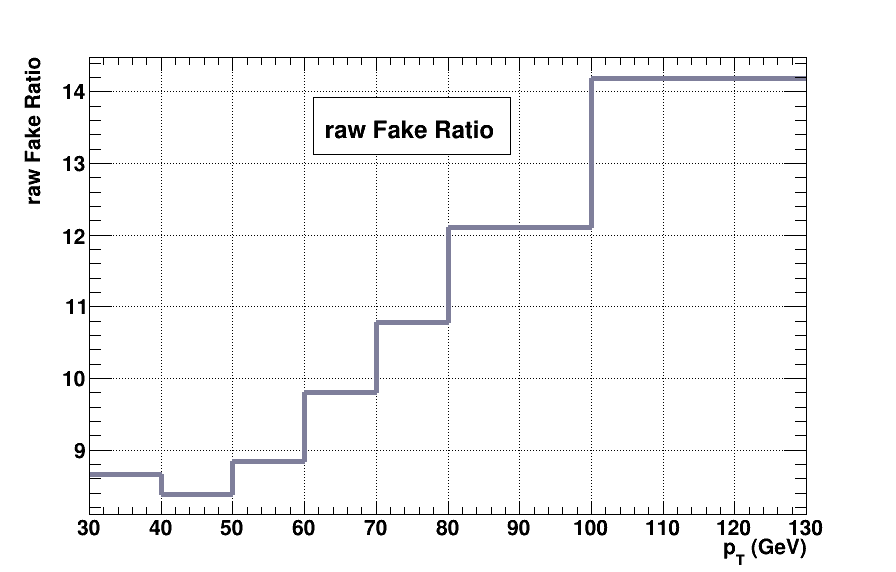
\includegraphics[width=0.6\columnwidth]{qcdPlots/qcd_rawFR.png}
\caption{Raw fake ratio values per photon \et bin.}
\label{fig:rawFR}
\end{center}
\end{figure}

%%%%%%%%%%%%%%%%%%%%%%%%%%%%%%%%%%%%%%%%%%%%%%%%%%%%%%%%%%%%%%%%%%%%%%%%%%%%%%%%%%%%%%%%%%%%%%%%%%%%%%%%%%%%%%%%%%%%%%%%%%%%%%%%%%%%%%%%%%%%%%%%%%%%%%%%%%%%%%%%%%%%%%
\subsubsection{Subtracting true photon contamination}

The numerator sample will be contaminated by a considerable fraction of true isolated photons from inclusive QCD direct photon production. This contribution needs to be estimated and subtracted to identify the true QCD fake ratio. We subtract these true photons using the template method. Due to this subtraction, the corrected fake ratio, then becomes:

\begin{equation}
FR_{corrected}=\frac{numerator-contamination}{denominator}
\end{equation}

The cleaning of the numerator of real photons is done through the template method. We use $\sigma_{i\eta i\eta}$ templates to distinguish between real and fake photons in the numerator sample. We construct our fake photon template by applying numerator like cuts to our data control sample (withtout the $\sigma_{i\eta i\eta}$ cut) in a sideband region of charged hadron isolation :

\begin{itemize}
\item $2.0 GeV <$ PF Charged Hadron isolation$<6.0 GeV$
\end{itemize}

The extraction of the templates for real photon shapes is done using Monte Carlo samples. In particular we have used $\gamma +$ Jets MC, applying numerator cuts again 
without the $\sigma_{i\eta i\eta}$ requirement and taking the leading reconstructed photon object that is also matched in $\Delta R$ to a generated photon. 

%We have analyzed the following samples:

%\begin{itemize}
%\item {/G\_Pt-*to*\_TuneZ2star\_8TeV\_pythia6/Summer12\_DR53X-PU\_S10\_START53\_V7A-v1}
%\end{itemize} 

A $\sigma_{i\eta i\eta}$ correction prescription is applied to real templates in order to match data \cite{higgs2GammaAN}. 
In particular we rescale $\sigma_{i\eta i\eta}$ to 

\begin{equation}
\sigma_{i\eta i\eta}^{scaled} = 0.891832 \times \sigma_{i\eta i\eta} + 0.0009133
\label{eqn:fr}
\end{equation}

as recommended by the $H \rightarrow \gamma \gamma$ group. We construct the real (MC-gen matched), 
fake (data-sideband) and data (data-numerator) $\sigma_{i\eta i\eta}$ templates for seven different photon \et bins of:

\begin{equation}
 [30-40], [40-50], [50-60], [60-70], [70-80], [80-100], [100-130] \GeV
\end{equation}

A likelihood fit using ROOFIT is then performed, of $real + fake$ templates to $data$ templates per $\ET^{\gamma}$.
Fig. \ref{fig:medTemplates1} and \ref{fig:medTemplates2} show the templates per photon \et bin after performing the fit.

\begin{figure}[hbtp]
\begin{center} 
$\begin{array}{cc}
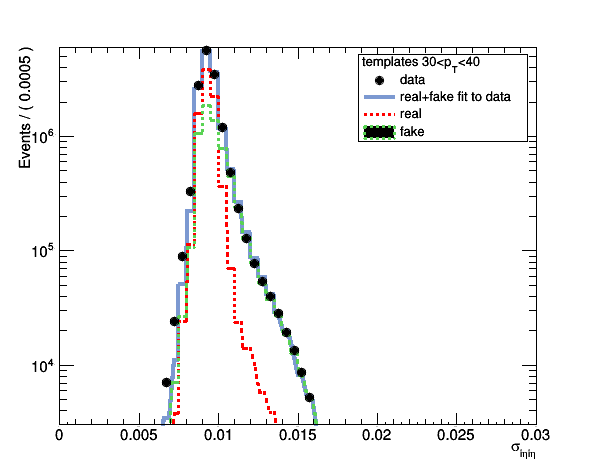
\includegraphics[width=0.4\columnwidth]{qcdPlots/qcd_template_1} &
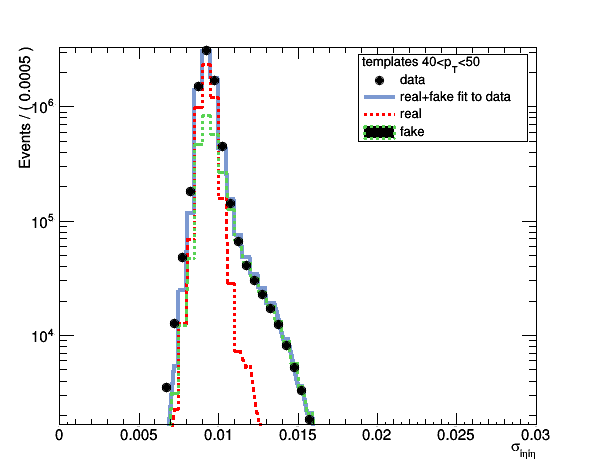
\includegraphics[width=0.4\columnwidth]{qcdPlots/qcd_template_2} \\
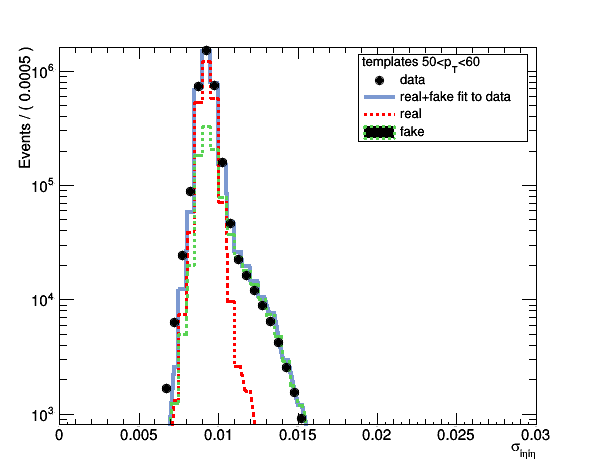
\includegraphics[width=0.4\columnwidth]{qcdPlots/qcd_template_3} &
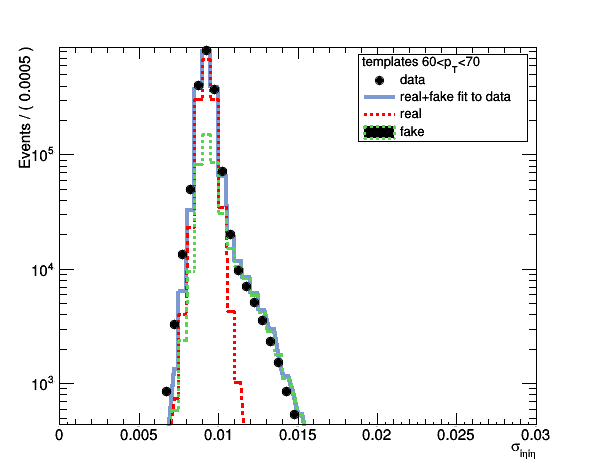
\includegraphics[width=0.4\columnwidth]{qcdPlots/qcd_template_4}
\end{array} $
\caption{$\sigma_{i\eta i\eta}$ templates for different photon \et bin.}
\label{fig:medTemplates1}
\end{center}
\end{figure}
%%-------------------------------------------------------------------------------
\begin{figure}[hbtp]
\begin{center} 
$\begin{array}{cc}
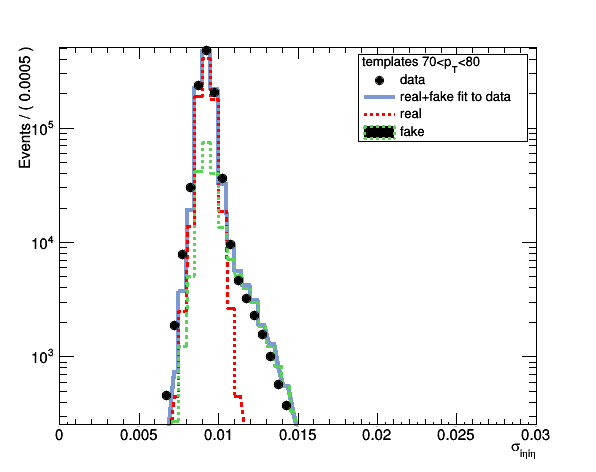
\includegraphics[width=0.4\columnwidth]{qcdPlots/qcd_template_5} &
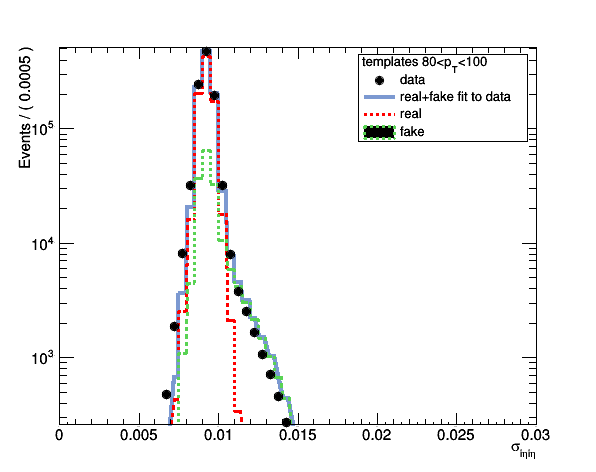
\includegraphics[width=0.4\columnwidth]{qcdPlots/qcd_template_6} \\
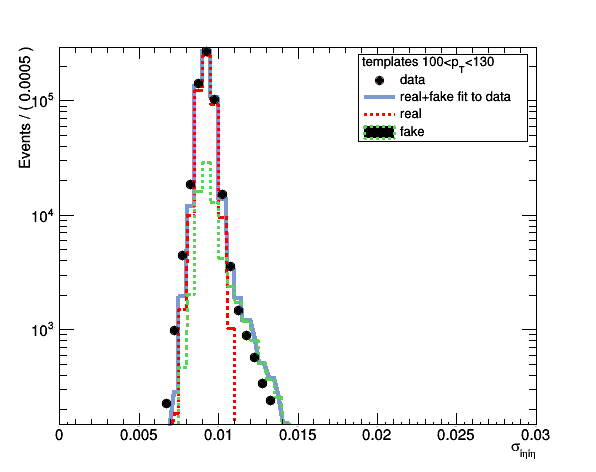
\includegraphics[width=0.4\columnwidth]{qcdPlots/qcd_template_7} &
\end{array} $
\caption{$\sigma_{i\eta i\eta}$ templates for different photon \et bin.}
\label{fig:medTemplates2}
\end{center}
\end{figure}

The yields of the real photons in the region of $\sigma_{i\eta i\eta}<0.011$ is called the contamination and is subtracted from the numerator yields, following equation~\ref{eqn:fr}.

%%%%%%%%%%%%%%%%%%%%%%%%%%%%%%%%%%%%%%%%%%%%%%%%%%%%%%%%%%%%%%%%%%%%%%%%%%%%%%%%%%%%%%%%%%%%%%%%%%%%%%%%%%%%%%%%%%%%%%%%%%%%%%%%%%%%%%%%%%%%%%%%%%%%%%%%%%%%%%%%%%%%%%
\subsubsection{Estimation of jet $\rightarrow$ photon mismeasurement ratio} 
As we have found the contamination in numerator, the corrected fake ratio is then calculated per photon \et bin, by simply subtracting the real photon contribution from raw numerator. We then perform a final fit for the seven FR bins and obtain the final corrected fake ratio as a function of \et.
The function we have used to parametrize the FR is;

\begin{equation}
f_{\ET^{\gamma}} = p0 + \frac{p1}{(\ET^{\gamma})^{p2}}
\end{equation}

Fig. \ref{fig:fitResult} shows the corrected fake ratio as a function of photon \et. It should be noted that, given our disjoint selection of numerator and denominator samples, these samples are not subset of each other. Therefore, one can expect a ratio $>$ 1.

\begin{figure}[hbtp]
\begin{center}
%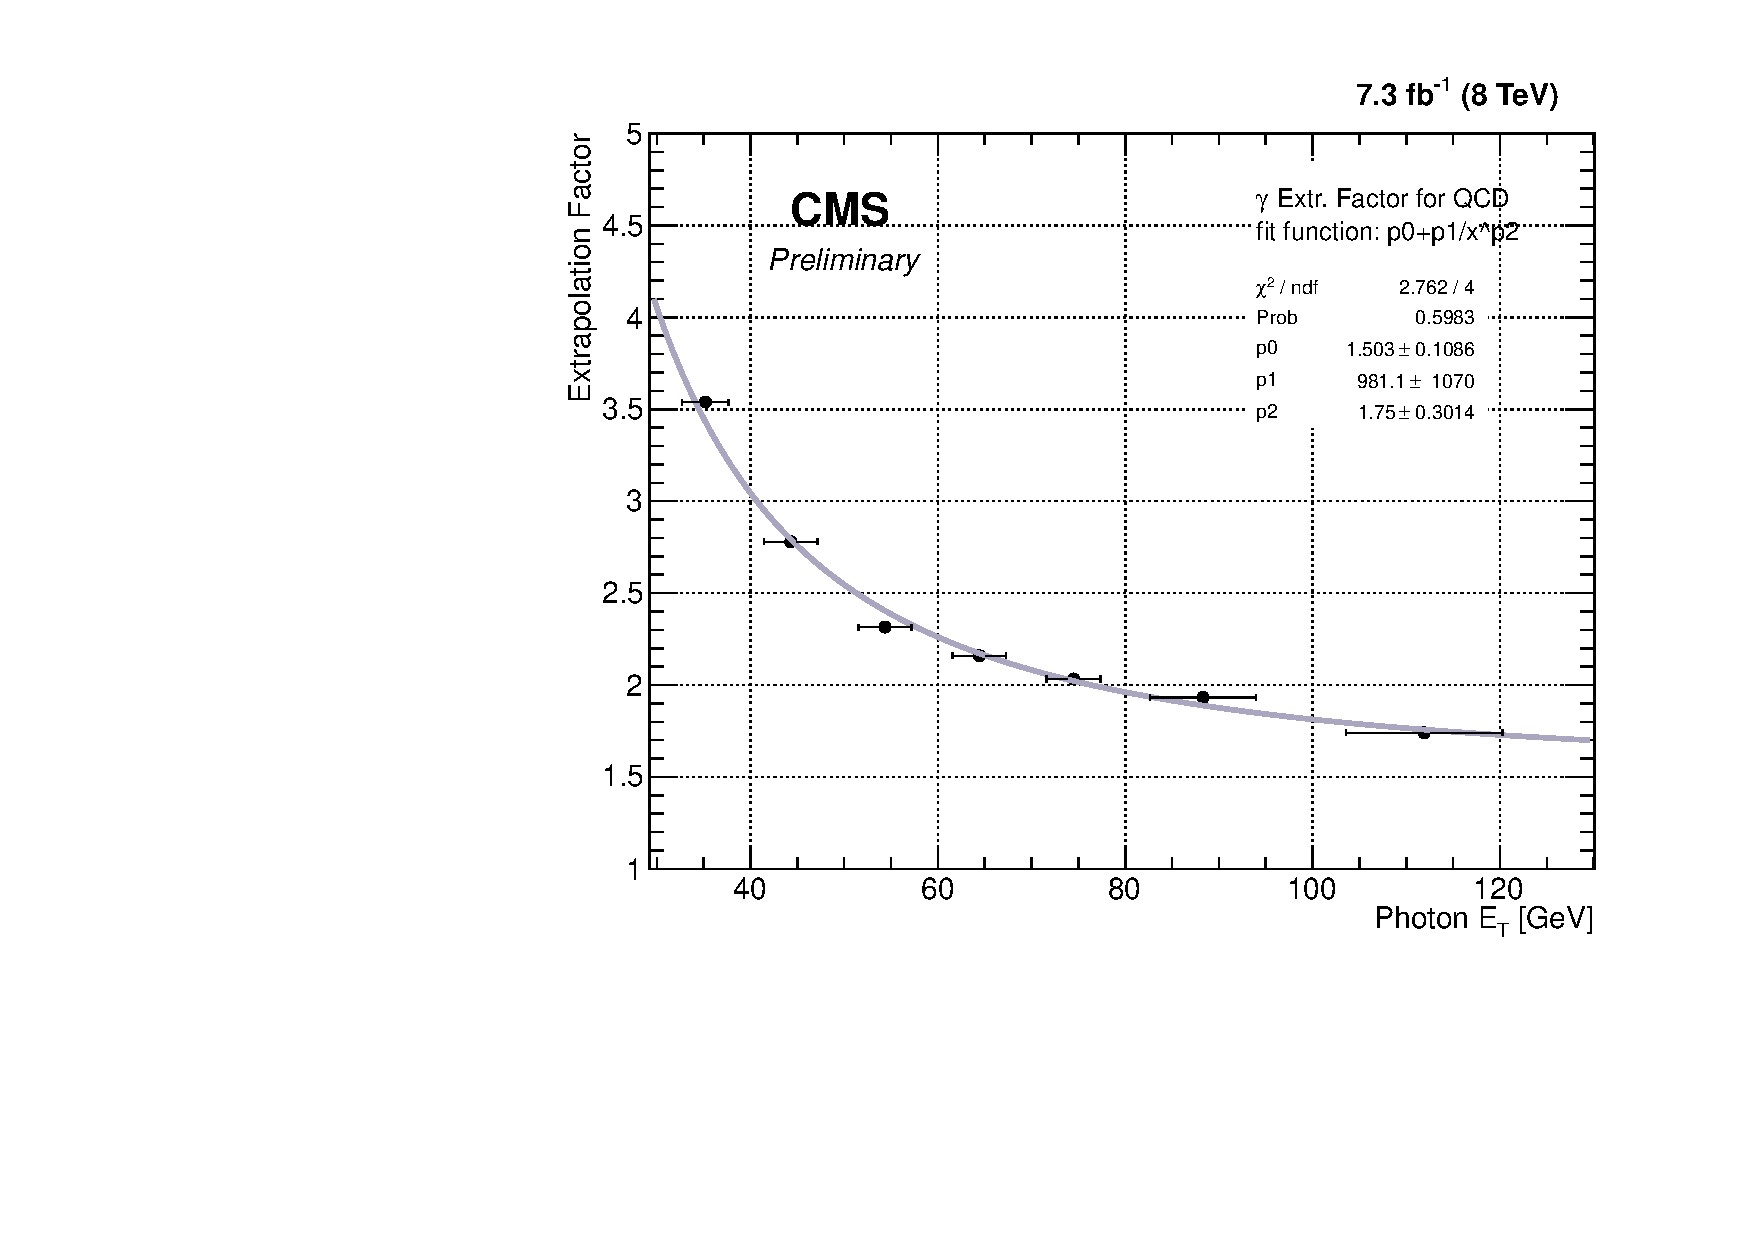
\includegraphics[scale=0.5]{qcd_plots/fitResult.pdf}
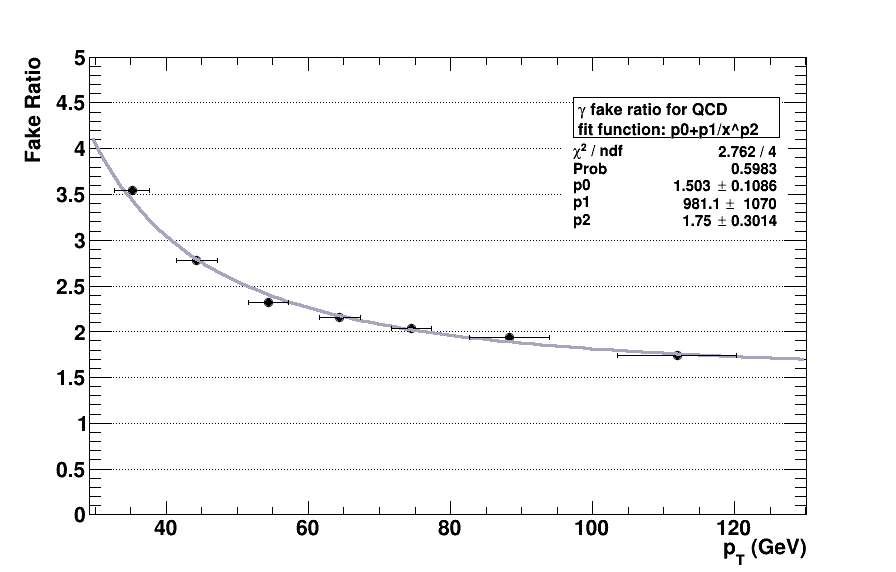
\includegraphics[scale=0.5]{qcdPlots/qcd_fitResult}
\caption{Final corrected fake ratio as a function of photon \et.}
\label{fig:fitResult}
\end{center}
\end{figure}

In this plot, the x-axis points and errors are calculated by looking at the mean and rms of the photon $\pt$ distribution in each $\pt$ bin. 
The errors on the y-axis are calculated through error propogation based on the fit errors. 
Finally, the QCD yield is estimated by applying the above function to the reconstructed photons of our analysis data sample,
which pass our basic selection cuts, but have the photon selection replaced by denominator selection cuts.

%%%%%%%%%%%%%%%%%%%%%%%%%%%%%%%%%%%%%%%%%%%%%%%%%%%%%%%%%%%%%%%%%%%%%%%%%%%%%%%%%%%%%%%%%%%%%%%%%%%%%%%%%%%%%%%%%%%%%%%%%%%%%%%%%%%%%%%%%%%%%%%%%%%%%%%%%%%%%%%%%%%%%%
\subsubsection{Jet $\rightarrow$ photon mismeasurement systematics} 
The main source of systematics on this procedure are estimated by examining the following;

\begin{itemize}
\item $\sigma_{i\eta i\eta}$ template binning
\end{itemize}

Template \textbf{binning} is examined and found to have almost negligible contribution. In particular we have recalculated the fake ratio by creating templates with half and
double bin size to estimate the photon contamination. This change in $\sigma_{i\eta i\eta}$ is found to not affect the final fake ratio estimate as can be seen in Fig. \ref{fig:fit_BINNINGsys}.

\begin{figure}[hbtp]
\begin{center}
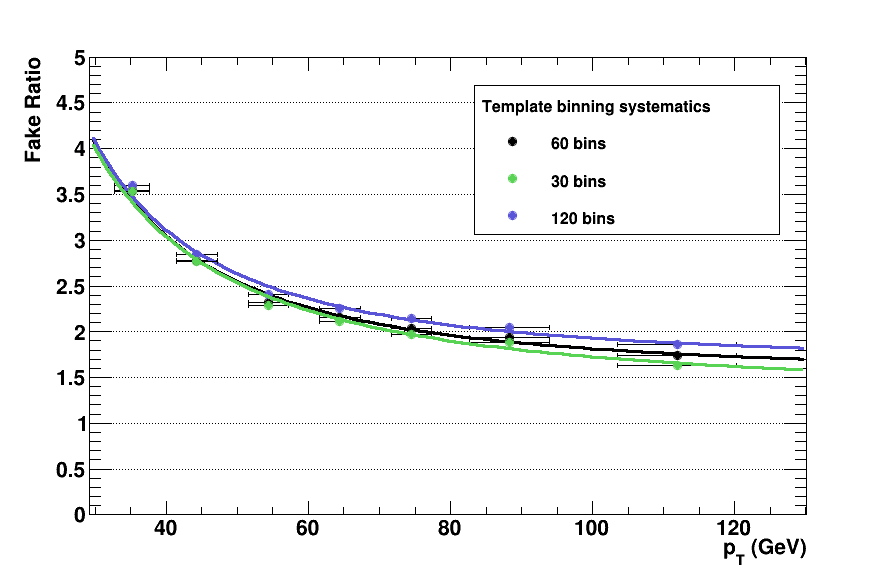
\includegraphics[width=0.7\columnwidth]{qcdPlots/qcd_fitResult_Binning}
\caption{Corrected fake ratio as a function of photon \et for different template binning.}
\label{fig:fit_BINNINGsys}
\end{center}
\end{figure}

\begin{itemize}
\item denominator definition
\end{itemize}

In order to calculate \textbf{denominator} systematics, we have altered the denominator definition by changing the lower bound definition of denominator selection cuts.
We have required one of the "OR" statements of the lower bound not to be present for each case. This has been performed for the PH and NH isolation statements in the lower bound criteria.  The following cuts are applied in both cases in their lower bounds:

\begin{itemize}
\item $ 0.015 > \sigma_{i\eta i\eta} > 0.012 $ \newline
\item\textbf{OR}  PF Charged Hadron Isolation $ > 4.0$ \newline
\item\textbf{OR}  PF Neutral Hadron Isolation $ > 4.5+0.04\times p_{T}^{\gamma}$ \newline
\end{itemize}

The cases differ by:
\begin{itemize}
\item {\bf Case I} : no PH isolation; \newline
\item {\bf Case II} : no NH isolation case; \newline
\end{itemize}

This procedure leads to a different denominator and as a result a different fake ratio as shown in Fig. \ref{fig:fit_DENOMsys} (left). 
However as mentioned above what is to be compared is the corresponding yield in our analysis data for denominator like objects. 
So different denominator leads to different yield. These final yields are plotted in Fig. \ref{fig:fit_DENOMsys} (right) for the different 
denominator cases and their difference is found to be negligible.

\begin{figure}[hbtp]
\centering
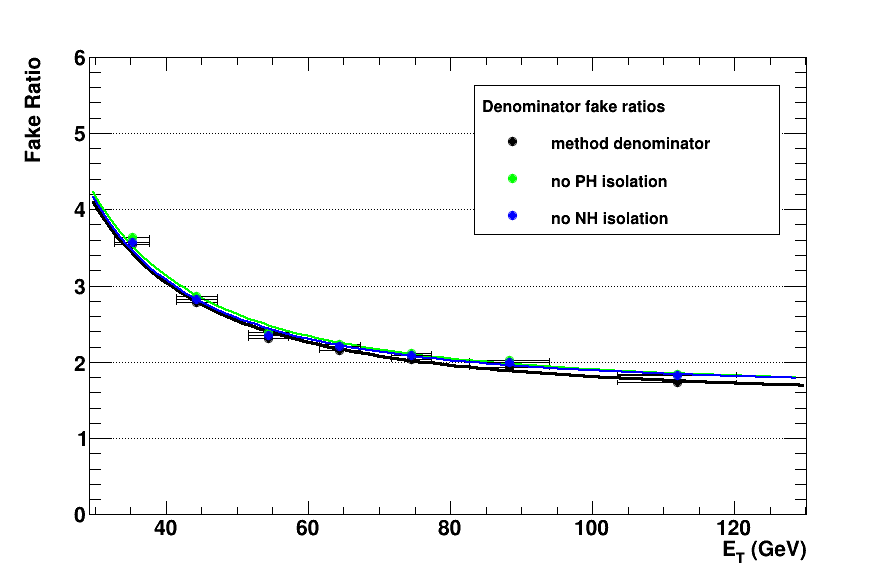
\includegraphics[width=0.45\textwidth]{qcdPlots/qcd_fitResult_deno}
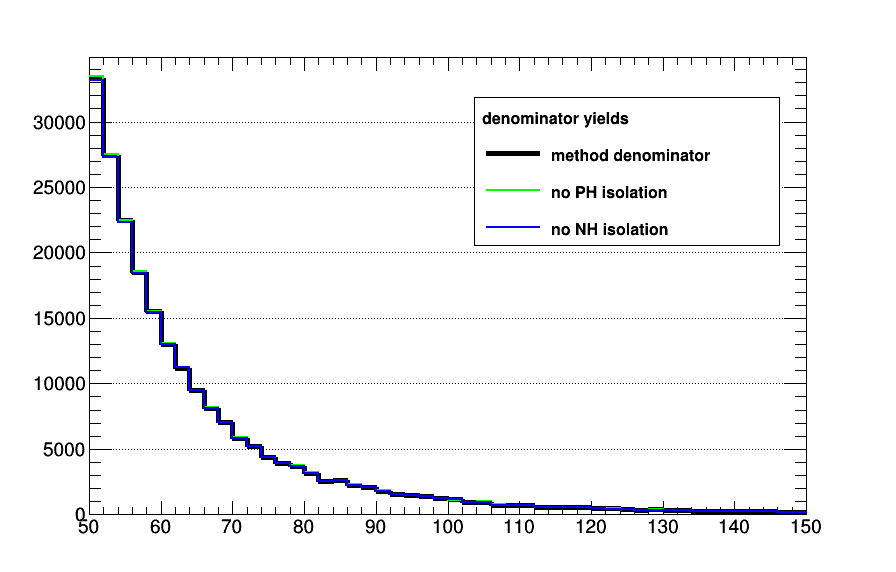
\includegraphics[width=0.45\textwidth]{qcdPlots/qcd_denoYields}
\caption{Corrected fake ratio as a function of photon \et for different denominator definitions and the final corresponding yields in our analysis data.}
\label{fig:fit_DENOMsys}
\end{figure}

\begin{itemize}
\item \met dependence
\end{itemize}

Regarding \textbf{missing transverse energy} dependence we have examined the dependence of the final fake ratio on \met.
We have calculated the fake ratio again as a function of both \met and $\ET^{\gamma}$. Fig. \ref{fig:fit_METsyspartial} shows the corresponding fake ratios as a function of $\ET^{\gamma}$ for various \met regions.  An additional test was made including our signal region, shown in figure \ref{fig:fit_METallsys}.

\begin{figure}[!h]
\begin{center}
{\label{fig:fit_METsyspartial}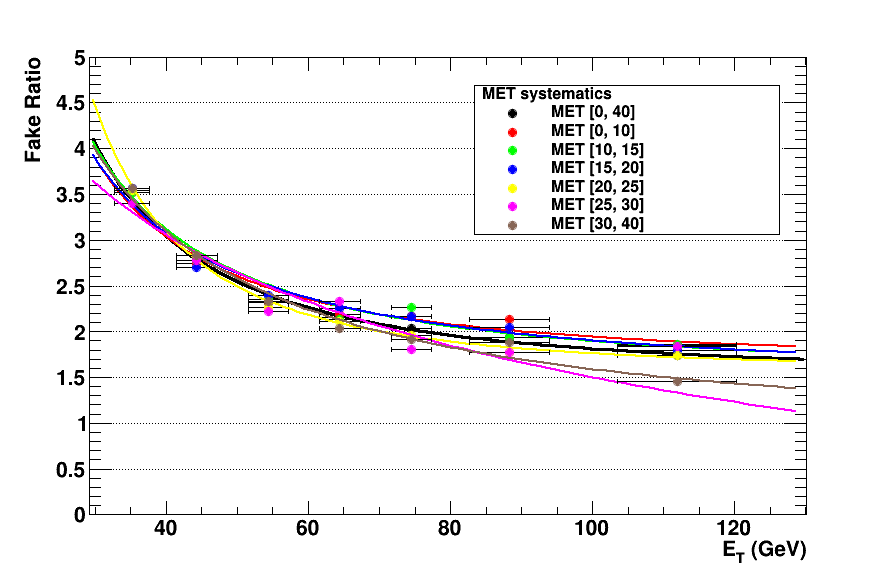
\includegraphics[width=0.45\textwidth]{qcdPlots/qcd_fitResult_MET40}}
{\label{fig:fit_METallsys}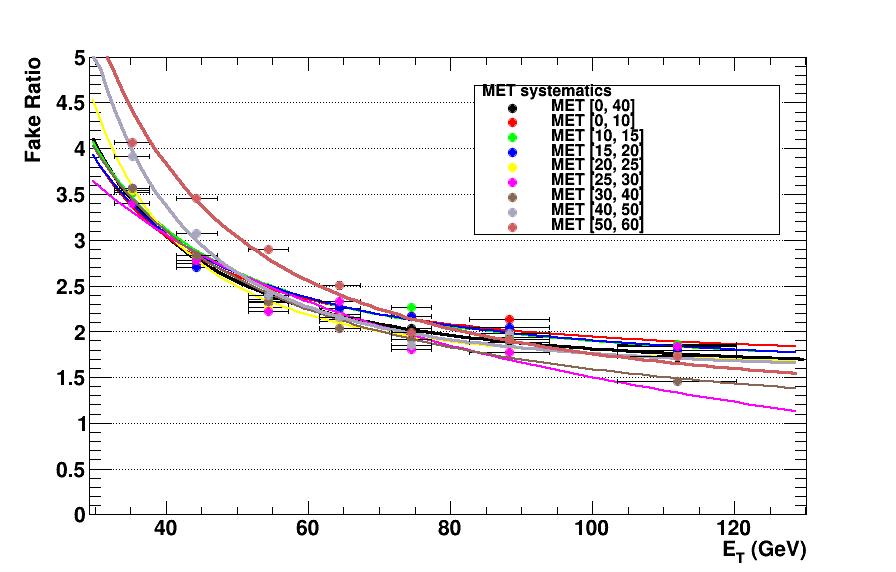
\includegraphics[width=0.45\textwidth]{qcdPlots/qcd_fitResult_allMET}}
\caption{Corrected fake ratio as a function of photon \et for different \met regions.}
\label{fig:fit_METsys}
\end{center}
\end{figure}

\begin{itemize}
\item Sideband selection for the fake templates
\end{itemize}

Finally to compute the systematics coming from the \textbf{sideband selection} for our fake templates we have recomputed the fake ratio changing the sideband selection, closer to the "real photon" region and closer to the "fake photon" region. Fig. \ref{fig:fit_SIDEBANDsys} shows the corresponding fake ratios.

\begin{figure}[hbtp]
\begin{center}
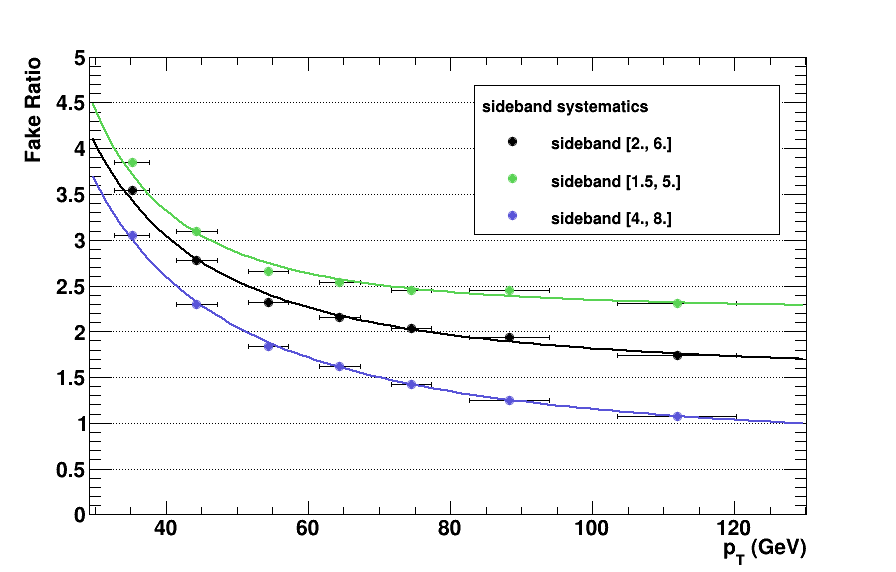
\includegraphics[width=0.7\columnwidth]{qcdPlots/qcd_fitResult_SB}
\caption{Corrected fake ratio as a function of photon \et for different sideband definitions.}
\label{fig:fit_SIDEBANDsys}
\end{center}
\end{figure}

As can be seen from above, the systematics associated with the sideband selection for our fake templates is proven to be the dominant one with ~35\%. This uncertainty is consistent with the other analysis (Exotica Diphoton and High Pt Monophoton) usign a similar approach to estimate jet faking photon background.

%%%%%%%%%%%%%%%%%%%%%%%%%%%%%%%%%%%%%%%%%%%%%%%%%%%%%%%%%%%%%%%%%%%%%%%%%%%%%%%%%%%%%%%%%%%%%%%%%%%%%%%%%%%%%%%%%%%%%%%%%%%%%%%%%%%%%%%%%%%%%%%%%%%%%%%%%%%%%%%%%%%%%%
\subsubsection{Closure test for jet $\rightarrow$ photon misidentification ratio measurement}

A closure test on the method was also performed in order to assure that our method closes well on MC.
We have performed the fake ratio method in our MC QCD samples and compared it with the fake ratio coming from MC truth information. 
The method and MC truth final fits and their ratio are presented in Fig. \ref{fig:qcd_closureTest1}.

%\begin{figure}[!h]
\begin{figure}[hbtp]
\begin{center}
%{\label{fig:qcd_closurefit}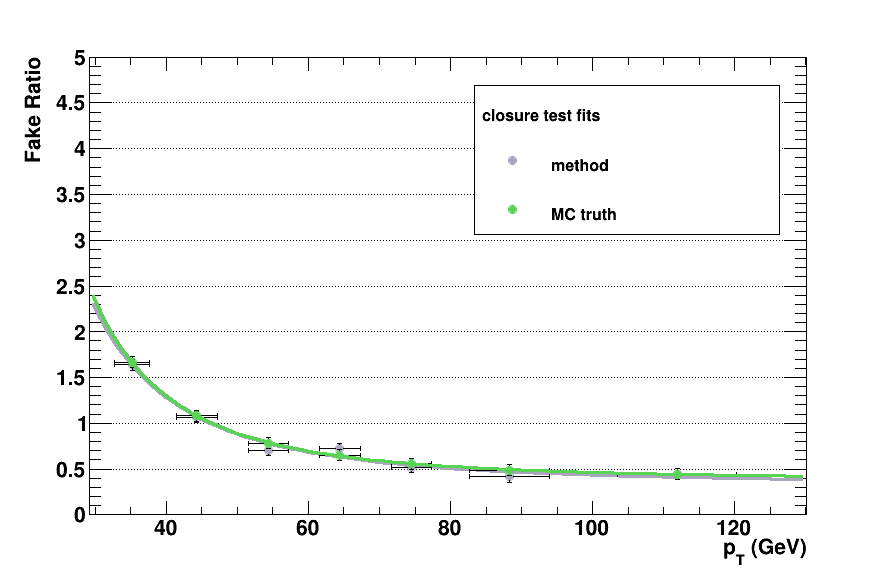
\includegraphics[width=0.45\textwidth]{qcdPlots/qcd_closureTest_fits}}
%{\label{fig:qcd_closureratio}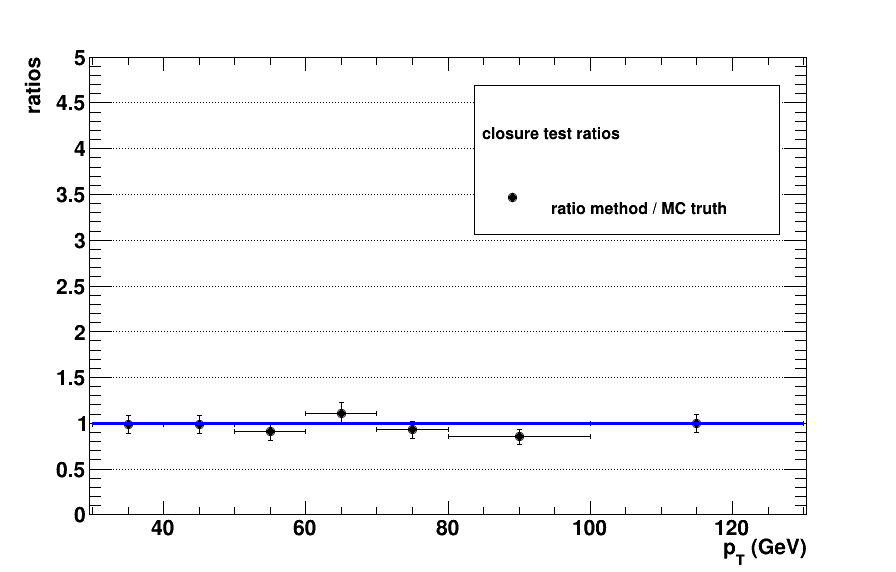
\includegraphics[width=0.45\textwidth]{qcdPlots/qcd_closureTest_ratio}}
%\caption{Closure test on the method. (a) Fake ratio method and MC truth fake ratio fits comparison and (b) their ratio, using QCD MC.}
%\label{fig:qcd_closure}
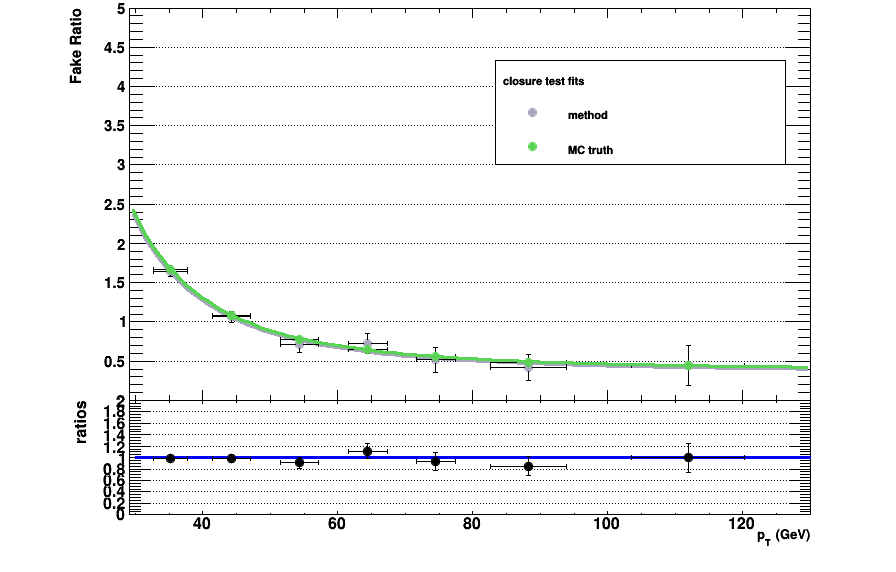
\includegraphics[width=0.7\columnwidth]{qcdPlots/qcd_closureTest1}
\caption{Closure test on the method. Fake ratio method and MC truth fake ratio fits comparison and their ratio, using QCD MC.}
\label{fig:qcd_closureTest1}
\end{center}
\end{figure}

In particular for the ratio method applyed on QCD MC we have constructed numerator, denominator and fake templates using QCD MC exactly as our data,
applying the same criteria as in our control sample. Real templates are again the ones used above, taken from $\gamma$ Jet sample.
Regarding MC truth ratio, this was constructed by using generated particle information and constructing the MC truth numerator and denominator, 
subtracting all real generated photons. The comparison of the method output to the truth fake ratio shows that our method closes very well.


%%%%%%%%%%%%%%%%%%%%%%%%%%%%%%%%%%%%%%%%%%%%%%%%%%%%%%%%%%%%%%%%%%%%%%%%%%%%%%%%%%%%%%%%%%%%%%%%%%%%%%%%%%%%%%%%%%%%%%%%%%%%%%%%%%%%%%%%%%%%%%%%%%%%%%%%%%%%%%%%%%%%%%
%%%%%%%%%%%%%%%%%%%%%%%%%%%%%%%%%%%%%%%%%%%%%%%%%%%%%%%%%%%%%%%%%%%%%%%%%%%%%%%%%%%%%%%%%%%%%%%%%%%%%%%%%%%%%%%%%%%%%%%%%%%%%%%%%%%%%%%%%%%%%%%%%%%%%%%%%%%%%%%%%%%%%%

In addition to that, a second closure test has been performed. This second test is intended to check the validity of the yields in the signal region. 
The procedure followed is described below. The general idea is to compare the QCD yield prediction of our method (fake ratio method) with the actual yield of fakes, on our candidate sample, which is obtained 
by reversing the \met cut, requirring $\met > 40 GeV$. As described above we apply the fake ratio function we have obtained, to objects passing denominator criteria 
in our candidate sample (i.e. $\met > 40 GeV$). In order to obtain the fake yield in our candidate sample, we construct 
numerator and fake templates per photon \et bin from our data, exactly as it is done in our method, apart from the $\met > 40 GeV$ cut. Real templates are again taken 
from MC, for $\met > 40 GeV$. We then again fit real and fake to numerator data and obtain the fake yield per photon \et bin, for $\sigma_{i\eta i\eta} < 0.011$. 
That means that by taking the ratio of fake yield over numerator yield for $\sigma_{i\eta i\eta} < 0.011$ we can obtain the fake fraction per photon \et bin in our 
candidate sample. We finally fit these bins and take the corresponding fake function for our candidate sample. Our candidate events are in fact numerator events with 
$\met > 40 GeV$ and $\sigma_{i\eta i\eta} < 0.011$. Applying this function on numerator events we obtain the yield of fakes in this sample. This yield is then compared
to the yield of fake ratio method. 

The fact that we are working on events with $\met > 40 GeV$, is making our samples sensitive to beam halo. In particular our templates are contaminated by beam halo events
as $\sigma_{i\eta i\eta}$ is left free in order to constuct the templates and perform the fitting. The $\sigma_{i\phi i\phi} > 0.001$ cut does not reject these events 
which are occuring at the area of $\sigma_{i\eta i\eta} > 0.015$. The above issue is shown in Fig. \ref{fig:template4_no_cut}.

\begin{figure}[!h]
\begin{center}
{\label{fig:template4_no_cut}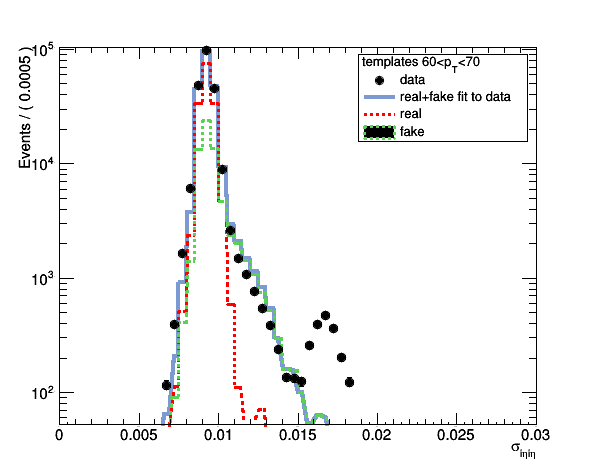
\includegraphics[width=5.5cm,height=4.3cm]{qcdPlots/template4_no_cut}}
{\label{fig:template4_sipip_cut}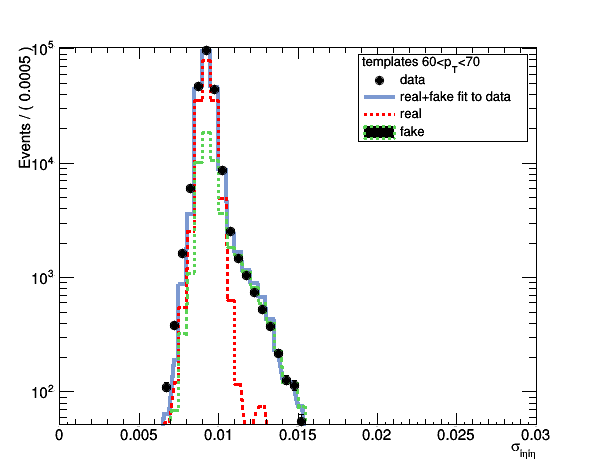
\includegraphics[width=5.5cm,height=4.3cm]{qcdPlots/template4_sipip_cut}}
{\label{fig:template4_sinin_cut}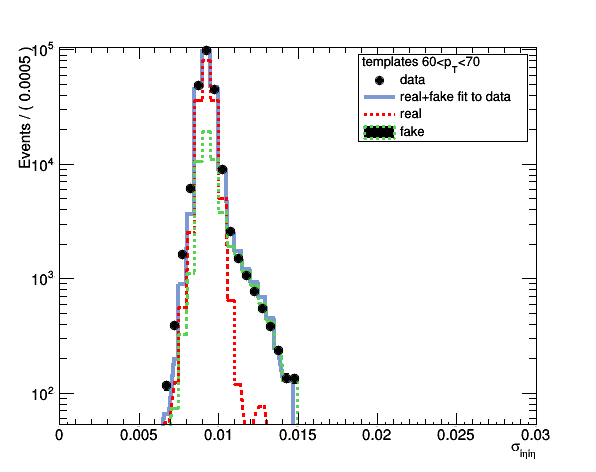
\includegraphics[width=5.5cm,height=4.3cm]{qcdPlots/template4_sinin_cut}}
\caption{$\sigma_{i\eta i\eta}$ templates for the 4th bin (a) without any harder cut, (b) with a harder $\sigma_{i\phi i\phi}$ cut, (c) with a $\sigma_{i\eta i\eta}$ cut.}
\label{fig:qcd_closure2_template4}
\end{center}
\end{figure}

The occurrence of beam halo events spoils our template fitting and as a result, the final fake yield. Fig. \ref{fig:template4_sipip_cut} shows the template fitting
for the same bin if a harder beam halo cut is applied, in particular $\sigma_{i\phi i\phi} > 0.009$. This results in rejecting mostly beam halo and obtaining a good fitting. 
However as we do not have a $\sigma_{i\phi i\phi} > 0.009$ cut in our analysis, we could find another way to reject it. In fact by observing that beam halo lives in the 
$\sigma_{i\eta i\eta} > 0.015$ area we could probably restrict our template area in the region of $0.001 < \sigma_{i\eta i\eta} > 0.015$. The corresponding template fitting 
is shown in Fig. \ref{fig:template4_sinin_cut} for the fourth bin. Of course we should prove that these two methods give the same results.

\begin{figure}[hbtp]
\begin{center}
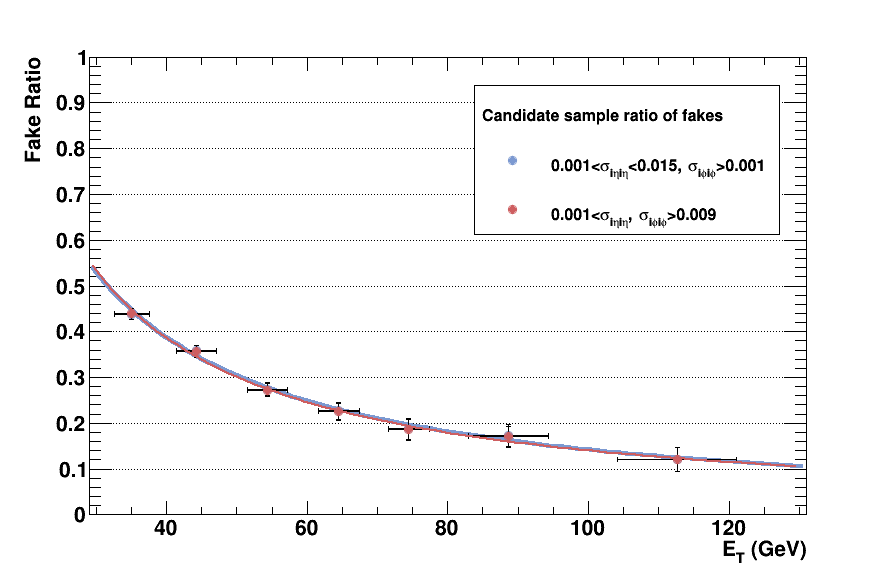
\includegraphics[width=0.6\columnwidth]{qcdPlots/fakeRatioFits_Sipip_Sinin}
\caption{Comparison of the fake ratio functions on candidate sample by putting a harder $\sigma_{i\phi i\phi}$ or a harder $\sigma_{i\eta i\eta}$ cut in our templates.}
\label{fig:fakeRatioFits_Sipip_Sinin}
\end{center}
\end{figure}

Fig. \ref{fig:fakeRatioFits_Sipip_Sinin} shows that the results on the final fit are almost identical. The final function of fakes to be applied on numerator data is 
shown in Fig.~\ref{fig:fitResult_closure2}.
Finally we apply this fake ratio function to numerator and compare it to the method prediction. Fig.~\ref{fig:closeYields} shows the comparison of the yields of these  two methods and the corresponding ratio obtained by dividing the fake ratio yield to the yield of our method.

\begin{figure}[hbtp]
\begin{center}
{\label{fig:fitResult_closure2}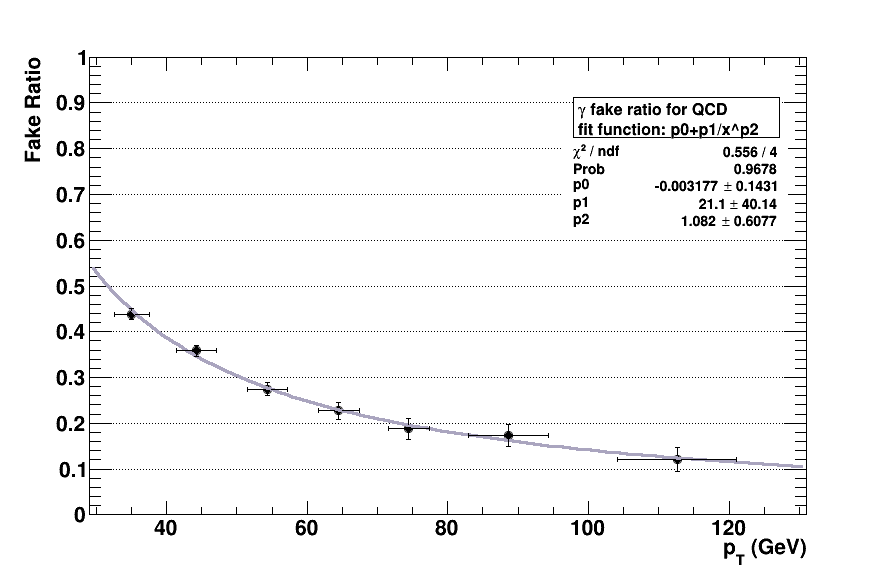
\includegraphics[width=0.45\textwidth]{qcdPlots/fitResult_closure2}}
{\label{fig:closeYields}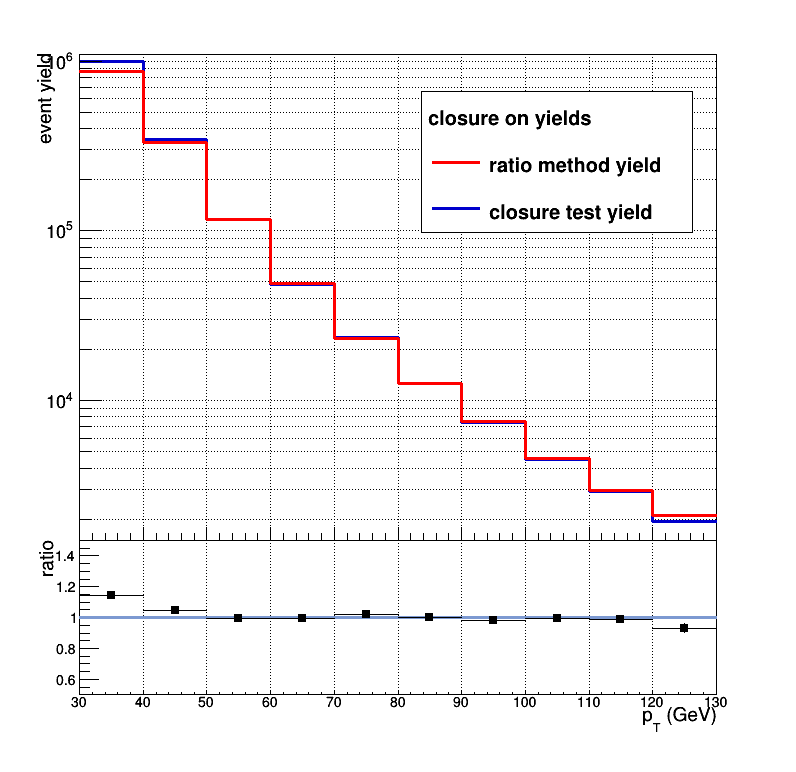
\includegraphics[width=0.45\textwidth]{qcdPlots/closeYields}}
\caption{Fit result of ratio of fakes in numerator data on the left, and comparision of the yields with on the right.}
\label{fig:fitResult_closure2_all}
\end{center}
\end{figure}

Through investigating various closure test methods, we have conlcuded that our estimations on the jet faking a photon background is reliable within the above mentioned systematics.

%%%%%%%%%%%%%%%%%%%%%%%%%%%%%%%%%%%%%%%%%%%%%%%%%%%%%%%%%%%%%%%%%%%%%%%%%%%%%%%%%%%%%%%%%%%%%%%%%%%%%%%%%%%%%%%%%%%%%%%%%%%%%%%%%%%%%%%%%%%%%%%%%%%%%%%%%%%%%%%%%%%%%%
%%%%%%%%%%%%%%%%%%%%%%%%%%%%%%%%%%%%%%%%%%%%%%%%%%%%%%%%%%%%%%%%%%%%%%%%%%%%%%%%%%%%%%%%%%%%%%%%%%%%%%%%%%%%%%%%%%%%%%%%%%%%%%%%%%%%%%%%%%%%%%%%%%%%%%%%%%%%%%%%%%%%%%


%%

After the cuts for QCD-like events are applied, the background that arises from electrons-faking-photons becomes the dominant for the kinematic range of this analysis. We have developed a data-driven method to obtain an accurate estimation of the electron-faking-photon background.
The main physical process behind this background is the $W\rightarrow e \nu$ production, which has a kinematic signature (fake photon \et, transverse mass, etc) very similar to the signal sample and large production cross section.

The method for estimating the electron-faking-photon contamination in the signal sample was done by constructing a control sample, similar to the signal sample, but enriched by electrons and not signal photons. This was achieved by reverting the pixel seed veto (PSV) in the photon ID requirements. The pixel seed veto cut is not the standard electron rejection tool in the $e-\gamma$ POG recommended photon ID; however, it has been shown to have a much smaller fake rate compared to the official electron rejection cut, the conversion safe electron veto. The PSV has been used in other photon-related analyses, such as the SUSY Photon and Exotica High Pt Monophoton analysis, in which the electron-faking-photon background is a dominant one.

After the control sample is created, it needs to be normalized by the number of expected electrons-faking-photons in the signal sample. This normalization can be obtained by the calculation of the fake rate of the PSV regarding electrons-faking-photons. It should be noted that this is not the fake rate of the full set of photon ID requirements, but only of the PSV cut. 

Before describing the details of this method, the following definitions must be made:

\begin{itemize}
\item $\gamma$: Objects that pass the complete $e/\gamma$ photon ID, including the PSV cut (photon object);
\item $\gamma_e$: Objects that pass the photon ID with the PSV cut reversed ($e$-fake object);
\item $N_{\gamma_e}$: Number of events in the control sample, which is made of $\gamma_e$;
\item $\epsilon_{\gamma_e}$: Efficiency of accepting $\gamma_e$ objects (including acceptance);
\item $\epsilon_{\gamma}$: Efficiency of accepting $\gamma$ objects (including acceptance);
\item $F_{e\rightarrow\gamma}$: Fake rate of the PSV cut for electrons-faking-photons.
\end{itemize}

Therefore, the number of electrons-faking-photons in the signal sample is given by
\begin{eqnarray}
N_{e \rightarrow \gamma} &=& \frac{N_{\gamma_e}}{\epsilon_{\gamma_e}} \times  F_{e\rightarrow \gamma} = N_{\gamma_e} \times R\\
R  &=& \frac{F_{e\rightarrow \gamma}}{\epsilon_{\gamma_e}}.
\end{eqnarray}

This ratio ($R$) can be related to the PSV fake rate because, for the PSV cut, the efficiency and fake rate obey the following relation:
\begin{eqnarray}
\epsilon_{\gamma_e} + F_{e\rightarrow \gamma} = 1.
\end{eqnarray}
Therefore,
\begin{eqnarray}
F_{e \rightarrow \gamma} = \frac{R}{1+R}.
\end{eqnarray}

The ratio and the fake rate can be measured using a tag-and-probe method. This method was applied to the SinglePhotonParked signal dataset. Analyzing events in which the $Z$ decays to electrons, we can reconstruct the number of events in four different cases:

\begin{itemize}
\item $Z_{e\gamma}$: one of the electrons of the $Z$ decay is identified an electron and the other is reconstructed as a photon object;
\item $Z_{e\gamma_e}$: one of the electrons of the $Z$ decay is identified as an electron and the other is reconstructed as an $e$-fake;
\item $Z_{\gamma_e\gamma}$: one of the electrons of the $Z$ decay is identified an $e$-fake and the other as a photon;
\item $Z_{\gamma_e \gamma_e}$:  both electrons of the $Z$ decay are identified as $e$-fakes;
\end{itemize} 

Therefore, we can reconstruct the number of events in each $Z$ peak case as:
\begin{eqnarray}
N_{e\gamma} &=& 2\times N^\prime\left( Z\rightarrow ee \right) \times  \epsilon_{e} \times F_{e\rightarrow\gamma}\\
N_{e\gamma_e} &=& 2\times N^\prime\left( Z\rightarrow ee \right) \times \epsilon_{e} \times \epsilon_{\gamma_e}\\
N_{\gamma \gamma_e} &=& 2\times N^\prime\left( Z\rightarrow ee \right) \times F_{e\rightarrow\gamma}\times \epsilon_{\gamma_e} \\
N_{\gamma_e \gamma_e} &=& N^\prime\left( Z\rightarrow ee \right) \times\epsilon_{\gamma_e}^2,
\end{eqnarray}
where $N_{xy}$ is the number of events of $Z$ decaying to electrons when the electrons are reconstructed as x and y, and $N^\prime\left( Z\rightarrow ee \right)$ overall number of expected $Z\rightarrow ee$ in the sample. The factors of two multiplying the first three equations are due to combinatorics.%related to the fact that there are two different objects to be identified and they can switch places.

With that system, we can infer that the calculation of the ratio can be performed in two ways:
\begin{eqnarray}
R  = \frac{F_{e\rightarrow \gamma}}{\epsilon_{\gamma_e}} = \frac{N_{e\gamma}}{N_{e\gamma_e}} = \frac{1}{2} \frac{N_{\gamma_e \gamma}}{N_{\gamma_e \gamma_e }}
\end{eqnarray}

The $Z$ shape was obtained from the template of a DY$\to ee$ MC at generator level. This template was then convoluted with a Gaussian to simulate detector resolution effects. The parameters of the Gaussian were then fitted to the obtained invariant mass distribution from the different categories detailed above. For the calculation of $N_{xy}$, the signal function was  integrated in the $\pm 2\sigma$ region to obtain the number of signal events. The fits for the $Z\rightarrow e \gamma$ and $Z \rightarrow e \gamma_e$ cases can be seen in Fig. \ref{Zep} and \ref{Zek}.
The background shape for the fit was estimated by the convolution of an error function and a decaying exponential function (RooCMSShape). The background in the Fig. \ref{Zep} is originated form the combinatorics of the electron plus non-resonant photon-like objects, such as real photons, jets faking photons and electrons faking photons originated from other interactions. Because the electron is most likely coming from the resonant Z production, the yield drops at lower values of $M_{e\gamma}$. The small disagreement between the fits and the data aroung $85$ GeV comes from the trigger and selection acceptances, since our trigger photon object selection is $30$ GeV and our probe selection \pt for this study is $35$ GeV. 

%\begin{table}[H]
%\begin{center}
%\begin{tabular}{| p{8cm} | c | c |}
%\hline
%Sample & Cross Section & Number of Events \\ \hline
%/DYToEE\_M\_20\_TuneZ2star\_8TeV \_pythia6\_v2/Summer12\_DR53X-PU\_S10 \_START53\_V7A-v1/AODSIM & 1510.0 pb & 18532820 \\ \hline
%\end{tabular}
%\caption{Sample used for gen-level template on signal fit.}
%\label{DYtoEEMC}
%\end{center}
%\end{table}

\begin{figure}[H]
\begin{center}
{\label{Zep}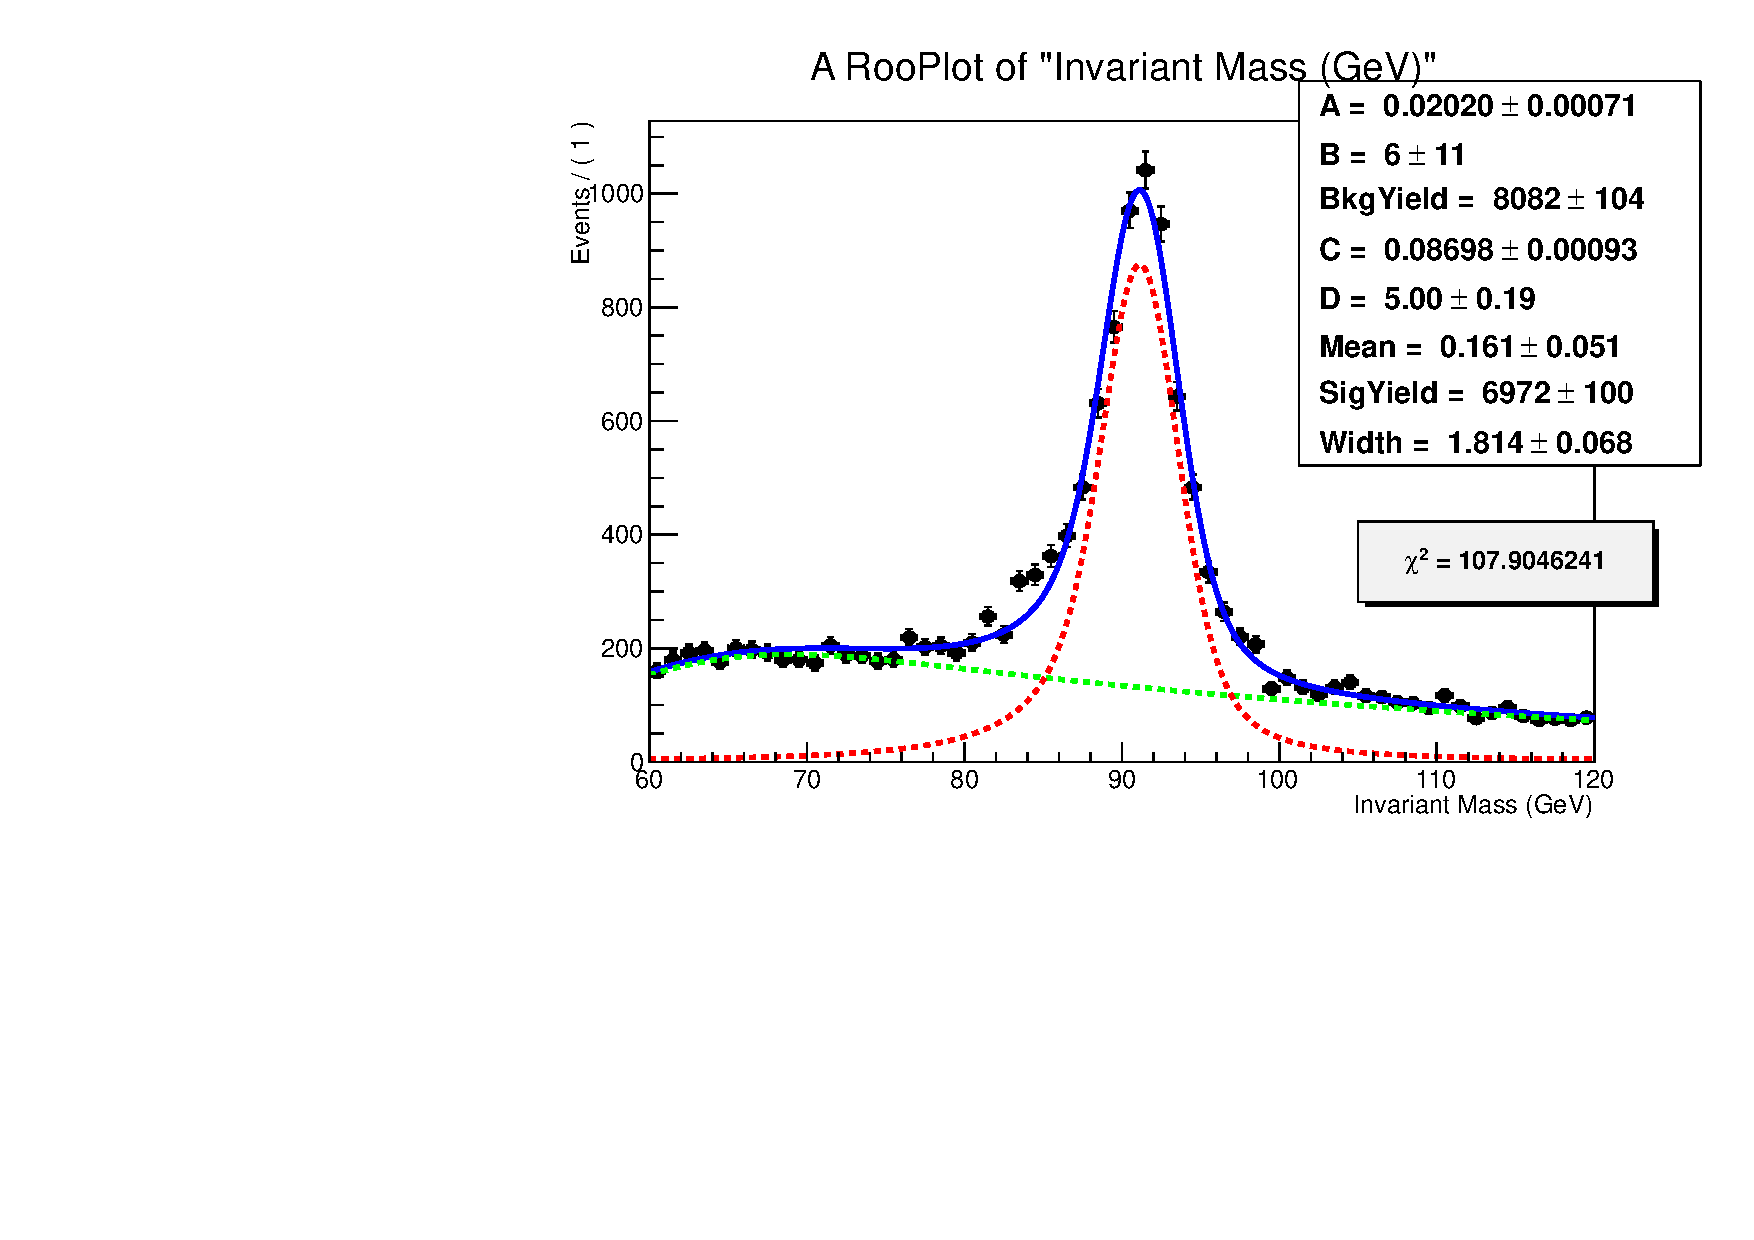
\includegraphics[width=0.45\textwidth]{efake_figs/Zep_FullMass.pdf}}
{\label{Zek}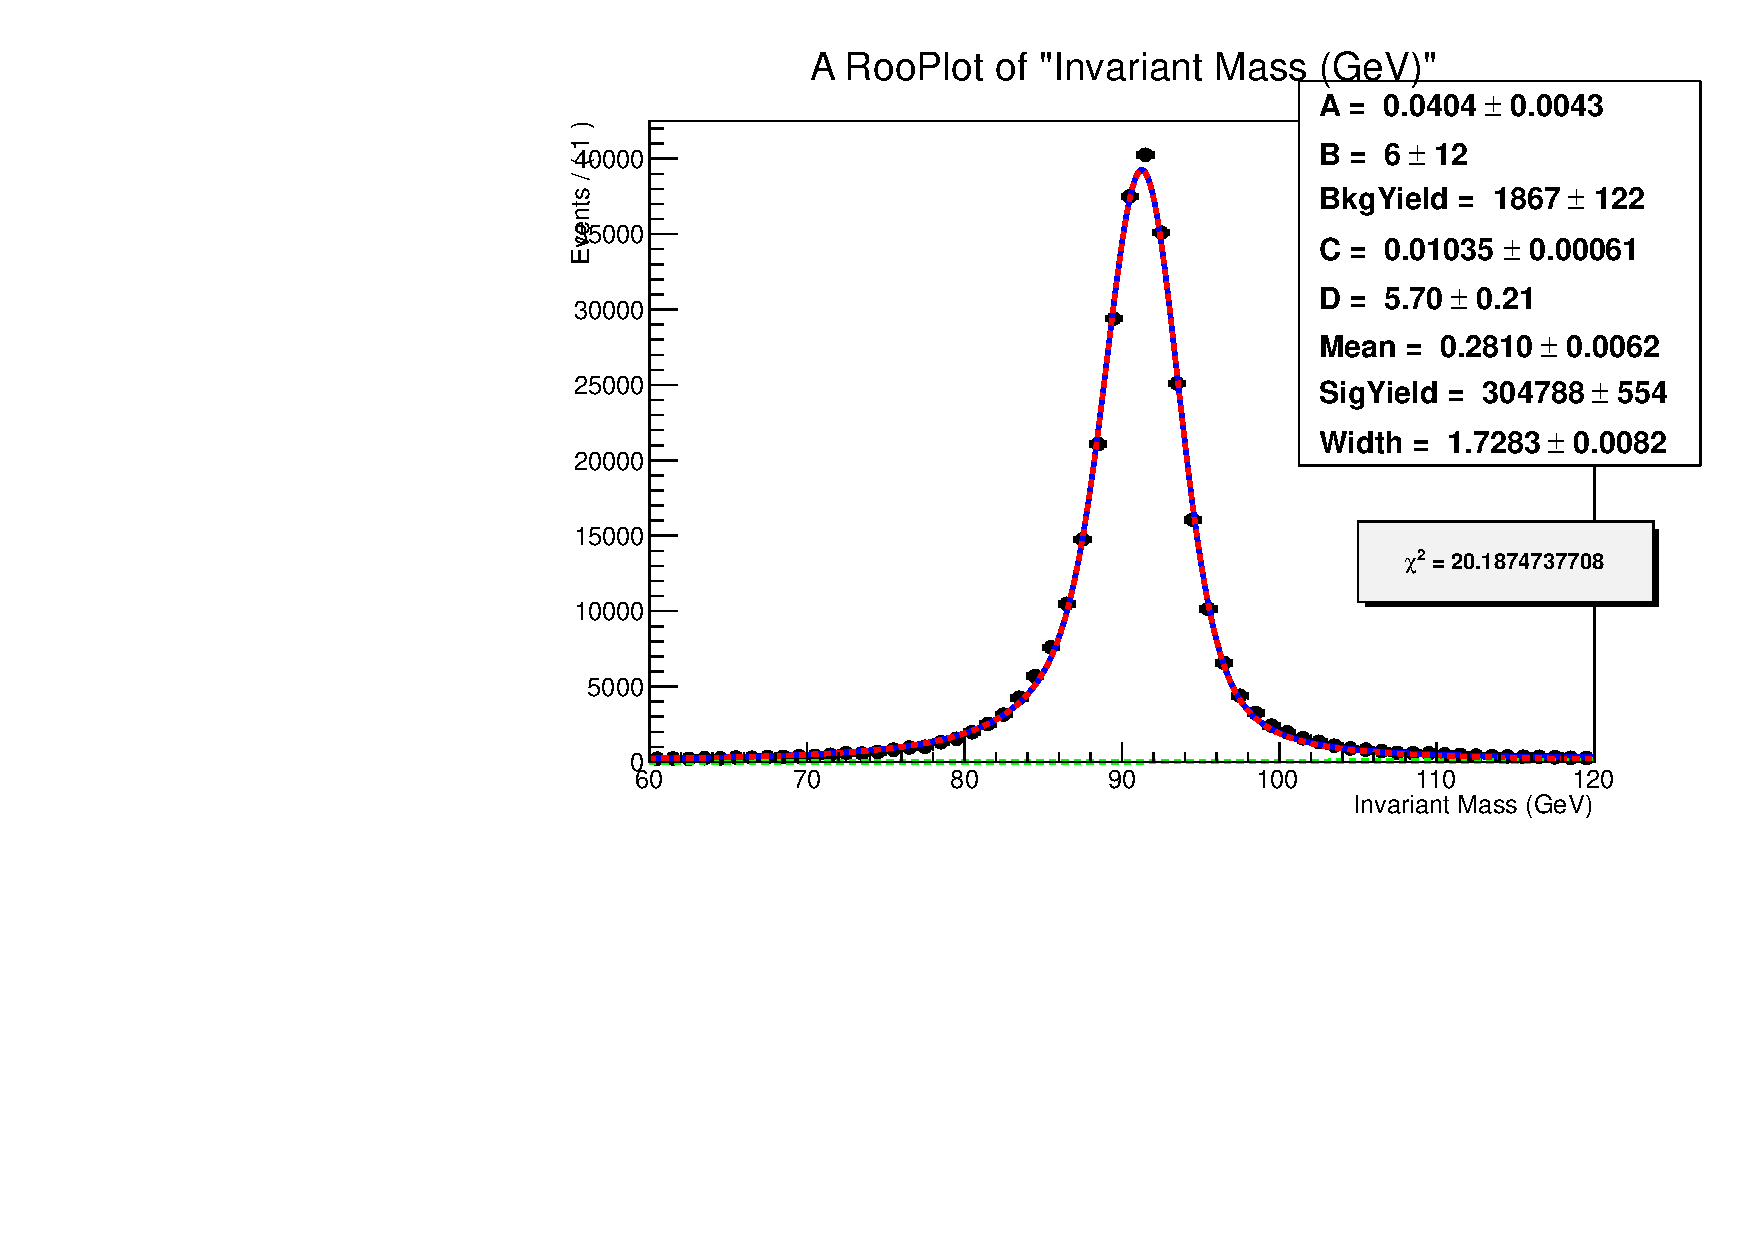
\includegraphics[width=0.45\textwidth]{efake_figs/Zek_FullMass.pdf}}
%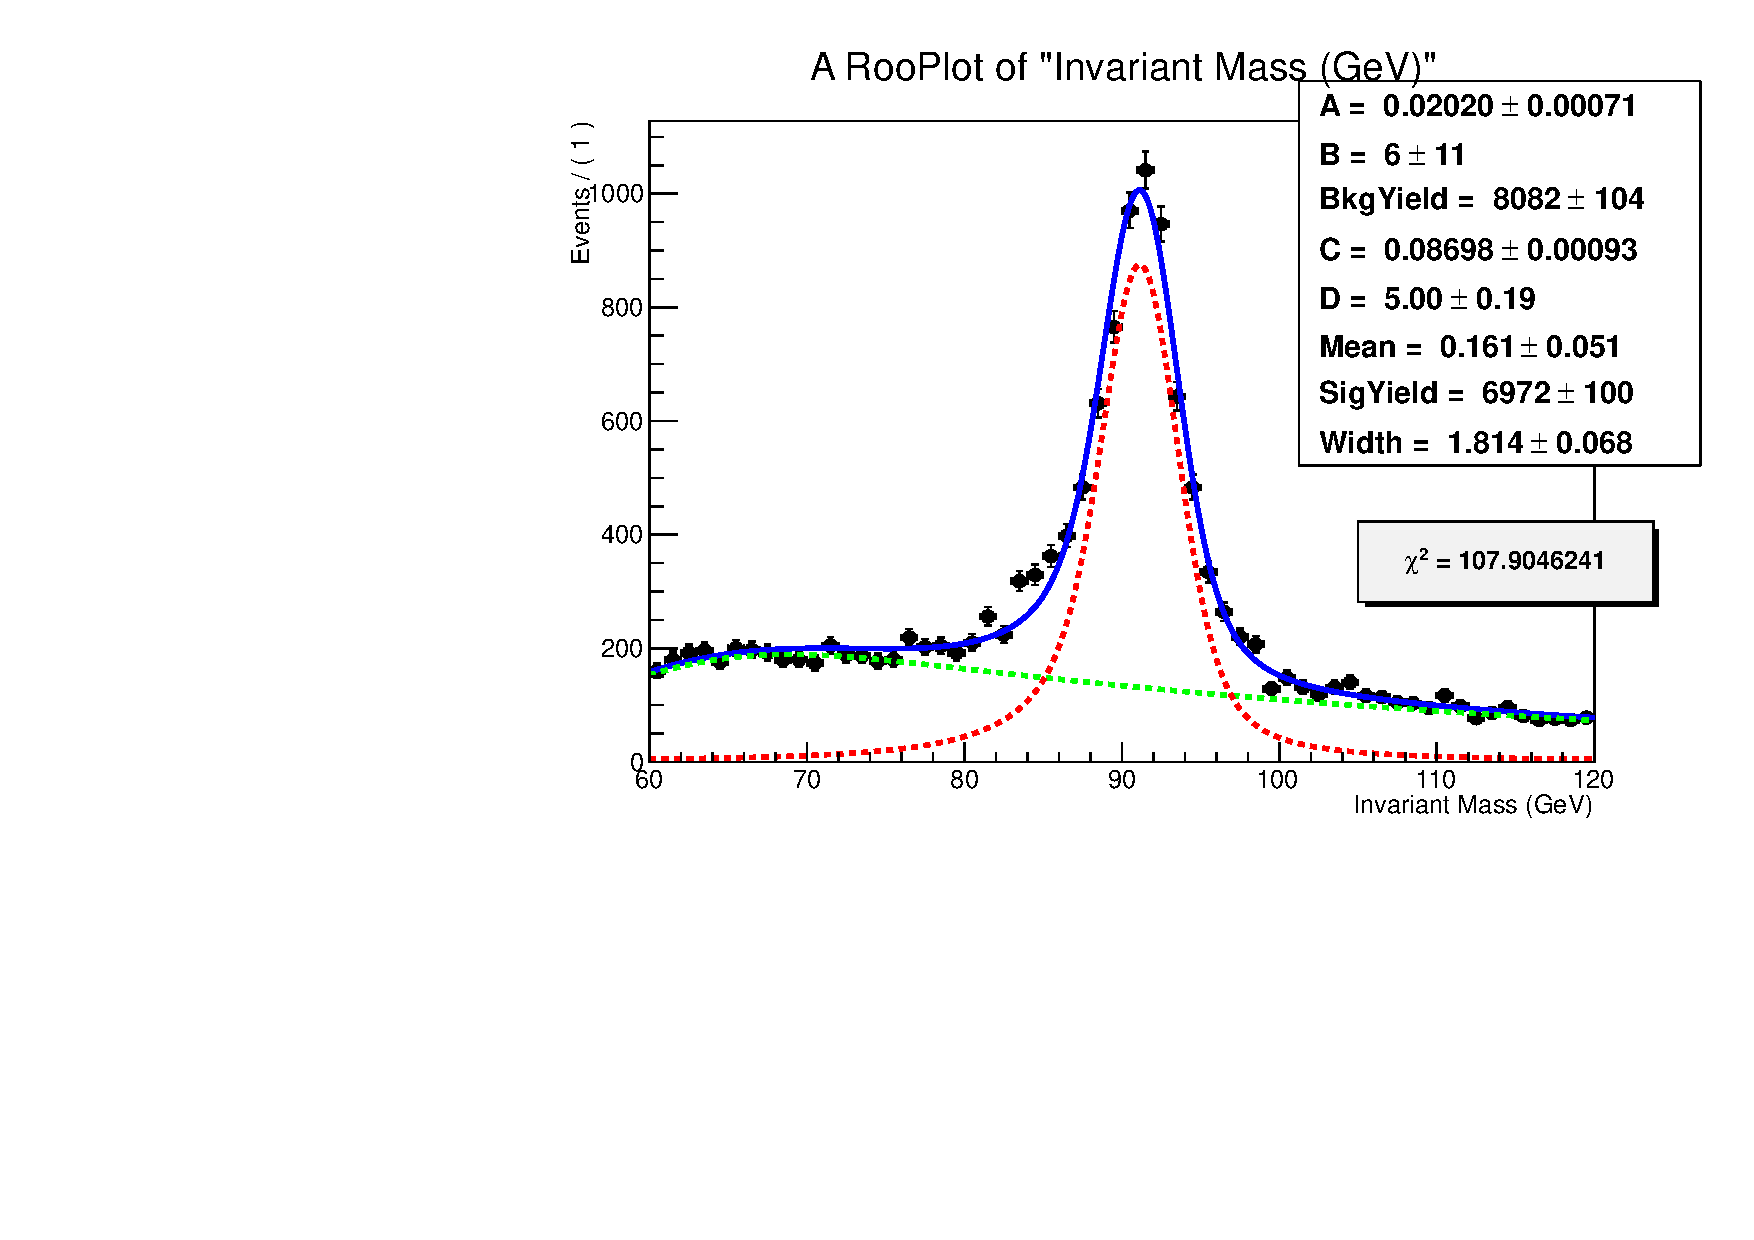
\includegraphics[scale=0.5]{efake_figs/Zep_FullMass.pdf}
\caption{Fit of the $Z$ invariant mass for the $Z\rightarrow e \gamma$ case and the $Z\rightarrow e \gamma_e$ case.}
\label{Zeall}
\end{center}
\end{figure}

%\begin{figure}[H]
%\begin{center}
%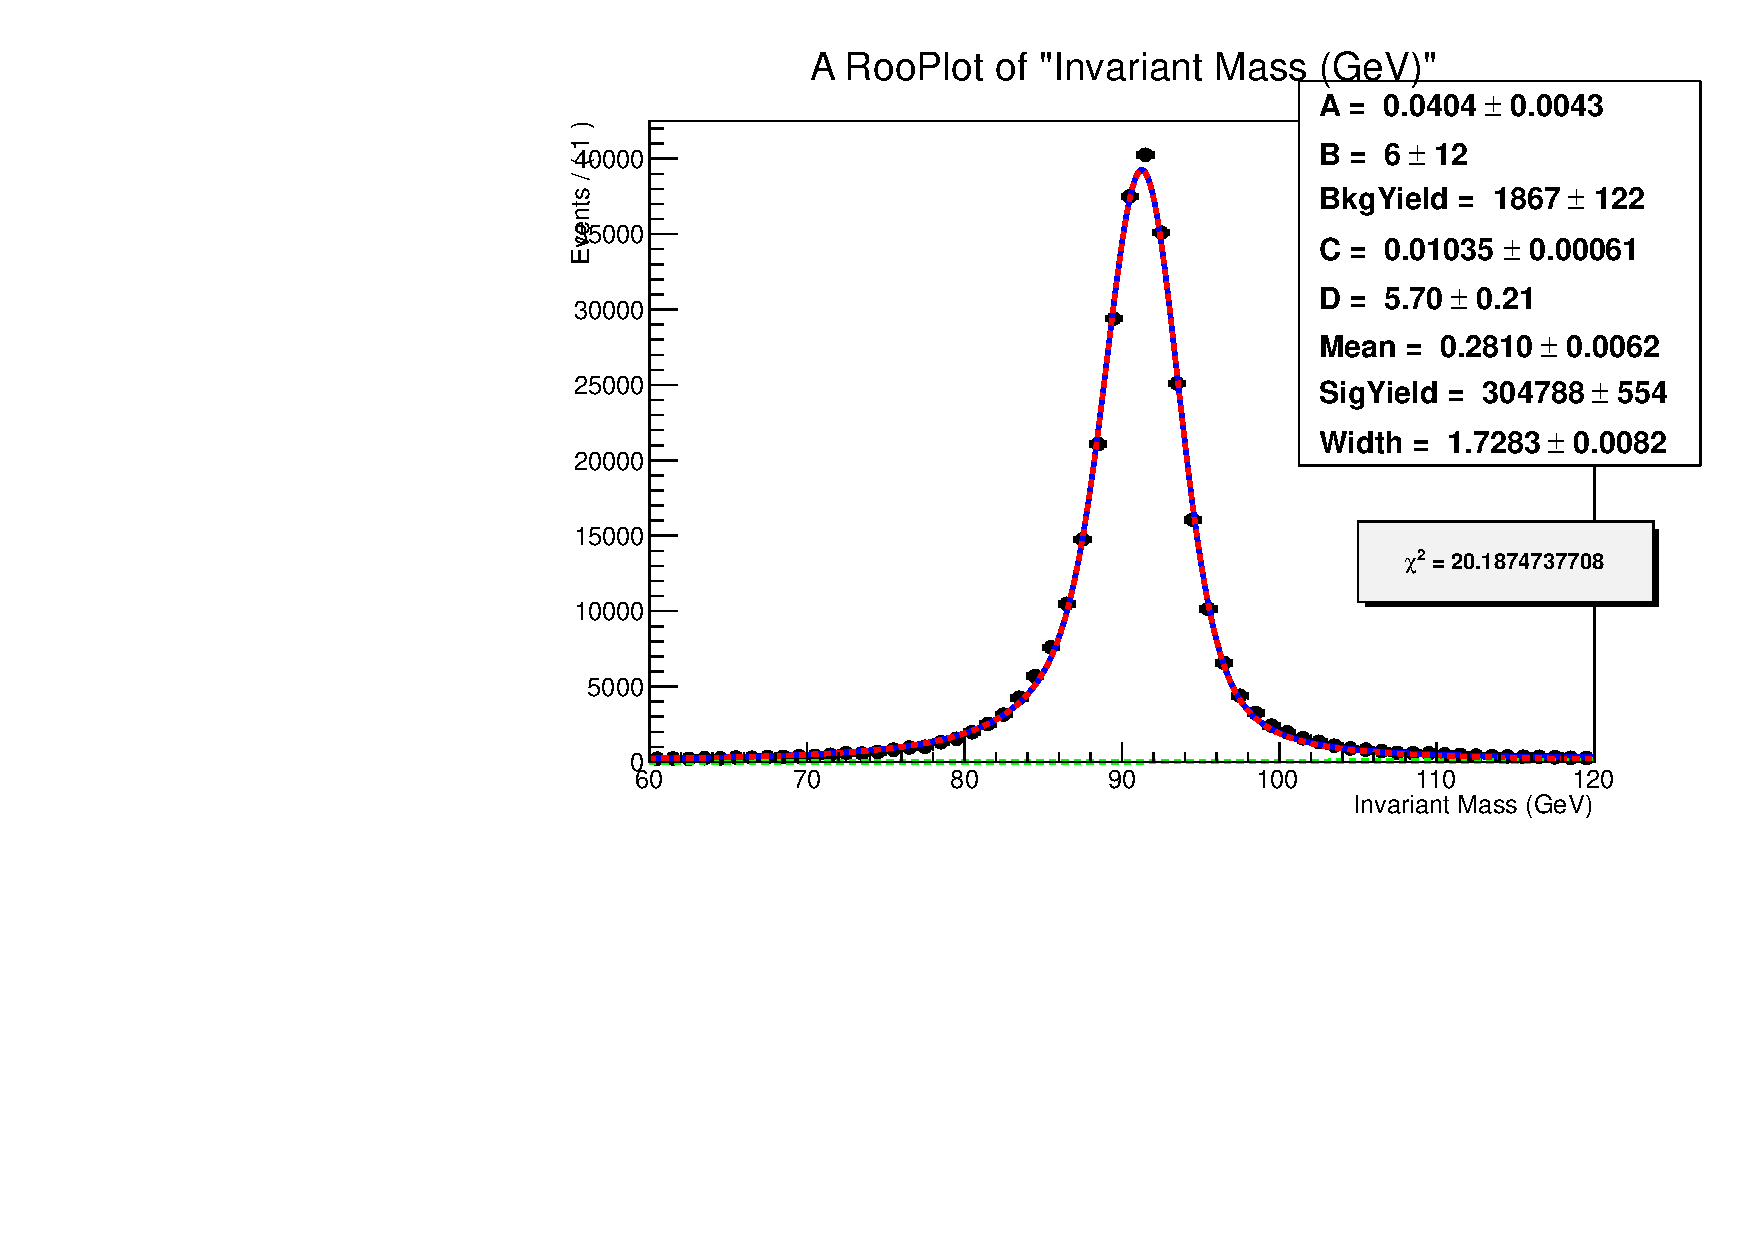
\includegraphics[scale=0.5]{efake_figs/Zek_FullMass.pdf}
%\caption{Fit of the $Z$ invariant mass for the $Z\rightarrow e \gamma_e$ case.}
%\label{Zek}
%\end{center}
%\end{figure}

Assuming a Poissonian error on the signal integral result, the error on the ratio and fake rate can be estimated as:

\begin{eqnarray}
\sigma_R &=& \sqrt{ \frac{1}{N_{e\gamma_e}^2}\sigma_{N_{e\gamma}}^2 + \frac{N_{e\gamma}^2}{N_{e\gamma_e}^4}\sigma_{N_{e\gamma_e}}^2 } \\
\sigma_{FR} &=& \frac{1}{\left( 1 + R \right)^2}\sigma_R.
\end{eqnarray}

With that, we obtain the following results:
\begin{eqnarray}
R &=& \left( 2.38 \pm 0.03 \right)\% \\
F_{e\rightarrow \gamma} &=& \left( 2.32\pm 0.03 \right)\%.
\end{eqnarray}

\subsubsection{Electron $\rightarrow$ Photon Fake Rate Dependencies on \pt, $N_{Vtx}$, $N_{Trk}$}

It has been shown before, in the environment of the SUSY Photon analysis, that the PSV fake rate is dependent on variables such as the probe $p_T$, the number of tracks associated with the primary vertex and the number of reconstructed primary vertices in the event. The nature of the two last dependencies are deeply rooted in the track reconstruction and matching algorithm. 

To check the dependency of the fake rate in the three variables mentioned, the fake rate was calculated in exclusive bins. In each bin, the signal template used was the corresponding bin in the MC signal sample. Each fit was done individually for every bin.

In the plots in Figure \ref{fig:FR_all}, we see how the PSV fake rate depends on the probe $p_T$, number of tracks associated with the primary vertex and the number of reconstructed primary vertices, respectively. The red line in each plot represents the fake rate obtained previously, assuming that there are no dependencies, with the entire invariant mass spectrum. For now on, this first result will be referenced as the flat fake rate.


\begin{figure}[H]
\begin{center}
{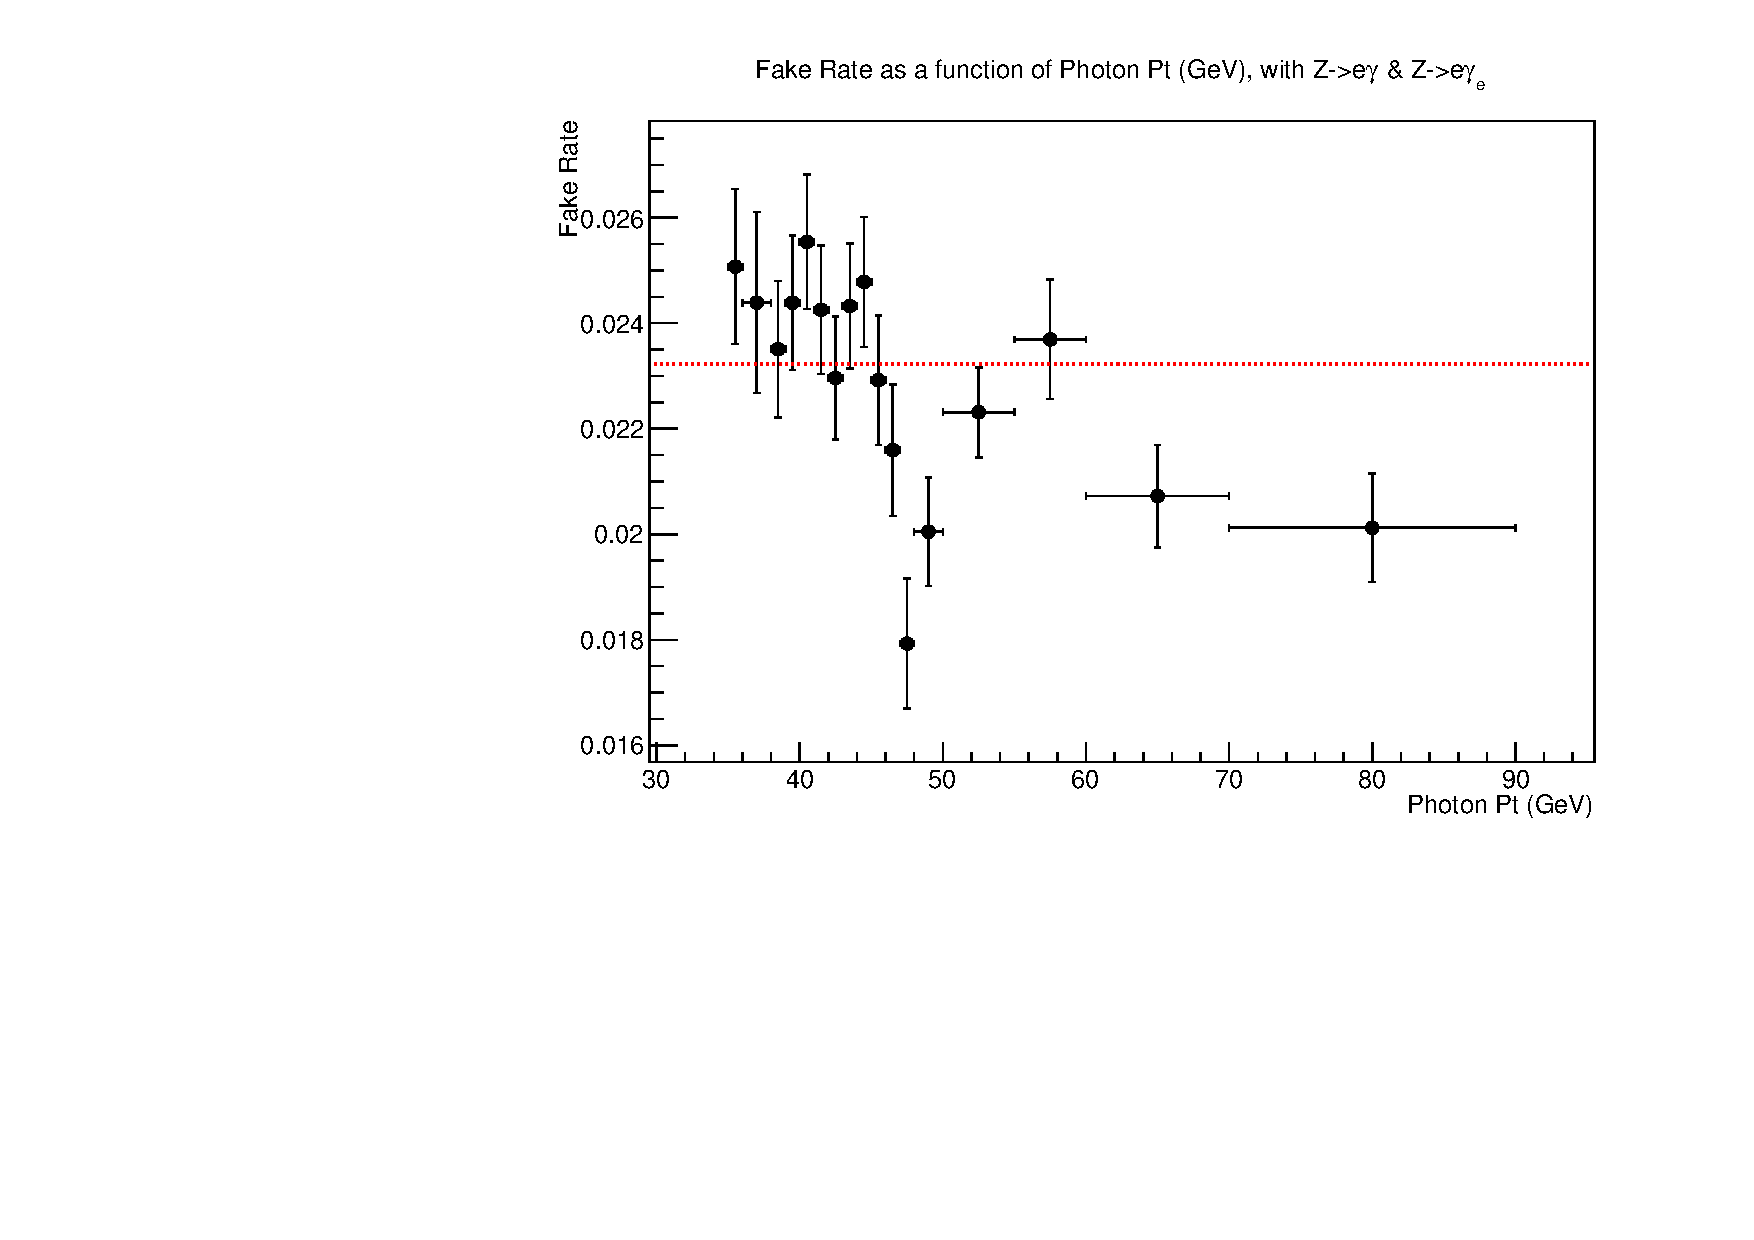
\includegraphics[width=0.45\textwidth]{efake_figs/FakeRate_Pt.pdf}}
{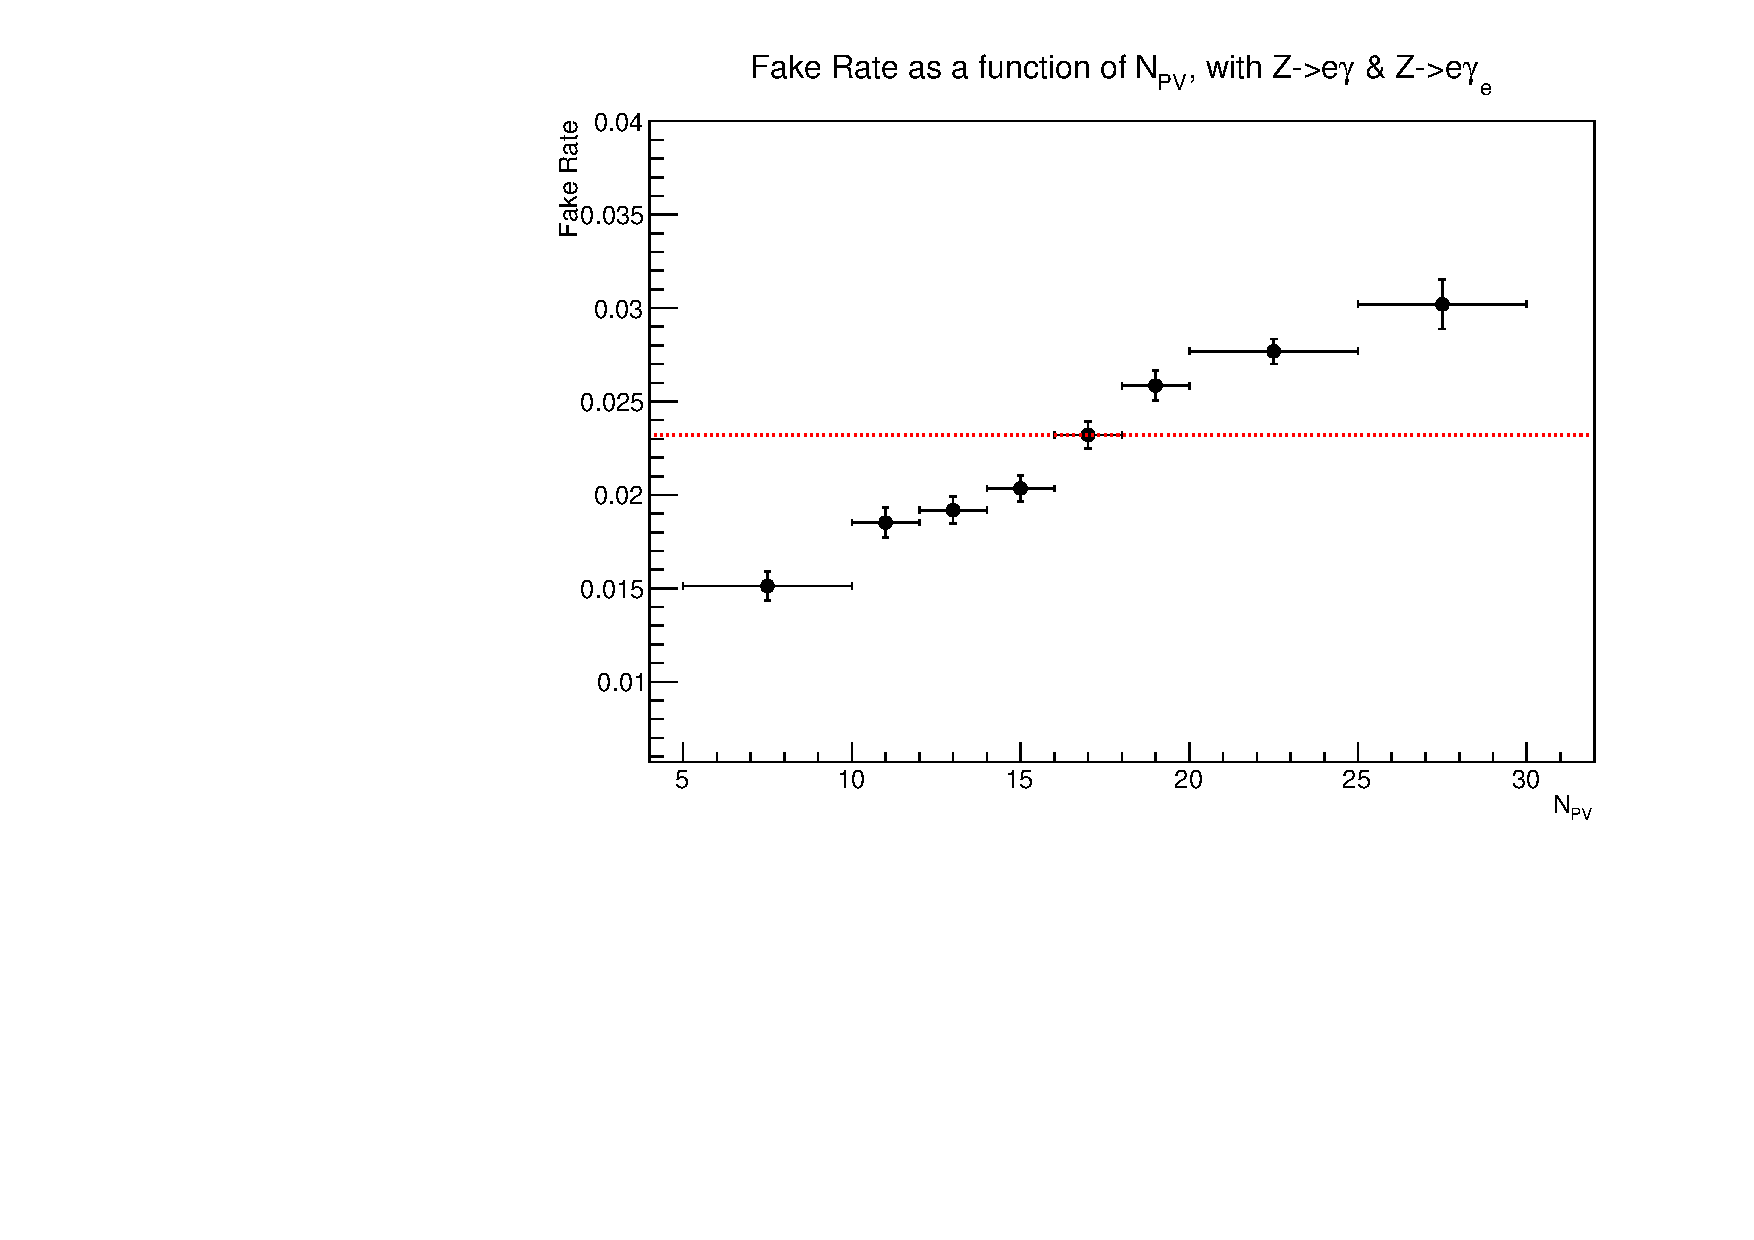
\includegraphics[width=0.45\textwidth]{efake_figs/FakeRate_PU.pdf}}
{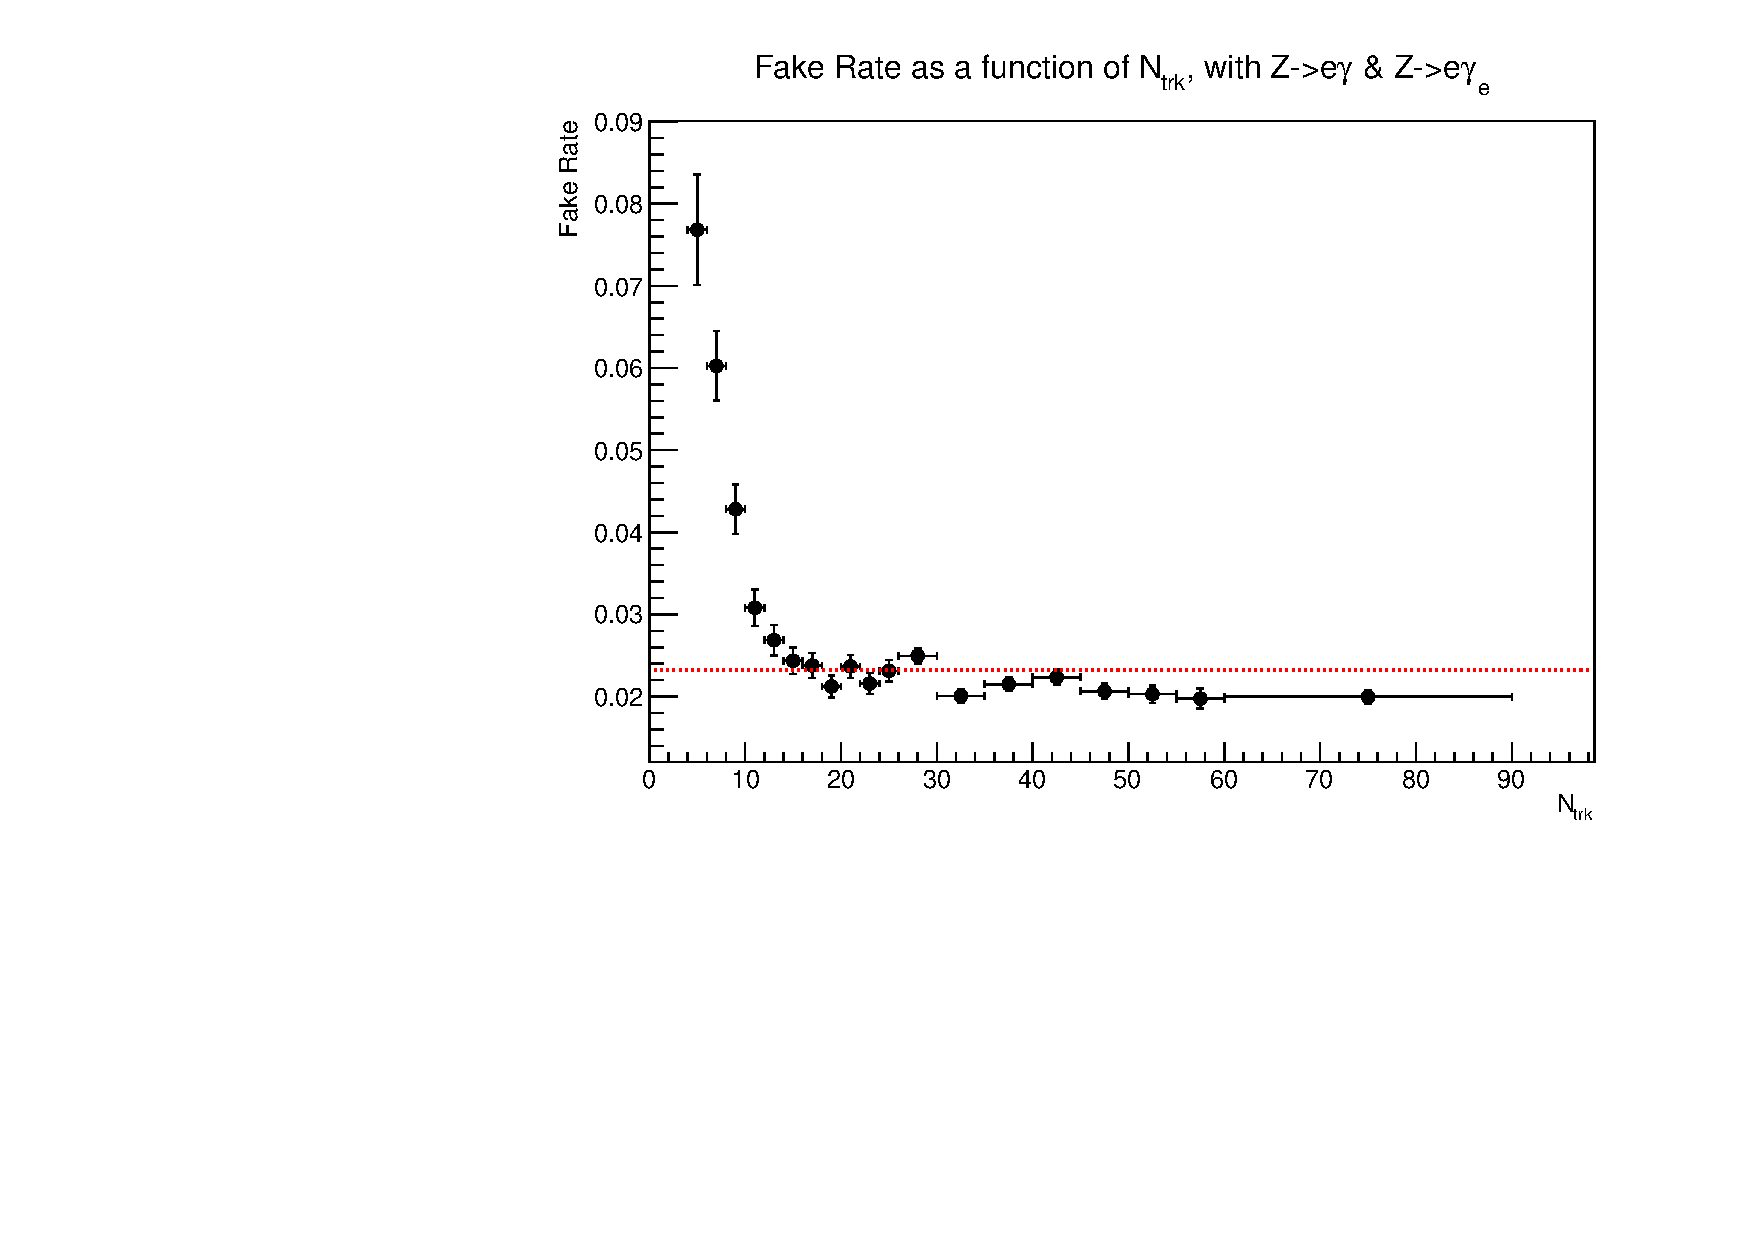
\includegraphics[width=0.45\textwidth]{efake_figs/FakeRate_Trk.pdf}}
\caption{Fake rate vs. probe $p_T$, number of primary vertices and track multiplicity.}
\label{fig:FR_all}
\end{center}
\end{figure}

As shown in the plots, there is a non-trivial dependency of the fake rate on the variables probed. There are different ways to solve this feature. The most complete one would be to achieve a multi-parameter description of the fake rate, including a 3-dimensional function with dependencies of the fake rate on each variable. That, however, demands a thorough study of these dependencies and a functional form to perform this task. A second way would be to choose one of the parametrizations, including the flat one, and prescribe a systematical error to that assumption. To know how much one choice impacts the fake rate, we can look at the final result and observe how much the yields change with each assumption.

In our case, the final result is the control sample of photon-like objects that fail the pixel seed veto normalized by the fake rate, which represents the estimation of our electron faking photon contamination in the signal region. The plots in Figure \ref{CS_params} show the shape and yields of this control sample when normalized by the different parametrizations of the fake rate. When checking the differences in number of events of each bin, we see that they are all within $5\%$ of each other, being higher around the $p_T$ peak and approaching $0$ for higher values. Therefore, it is safe to choose any specific parametrization and assume a systematic error of $5\%$ on the number of events to make sure that the different assumptions are compatible. With these assumptions, we choose to use the flat parametrization, since it only involves one fit and it has been shown to be much more stable with respect to different fit functions, for signal and background.


\begin{figure}[H]
\begin{center}
  {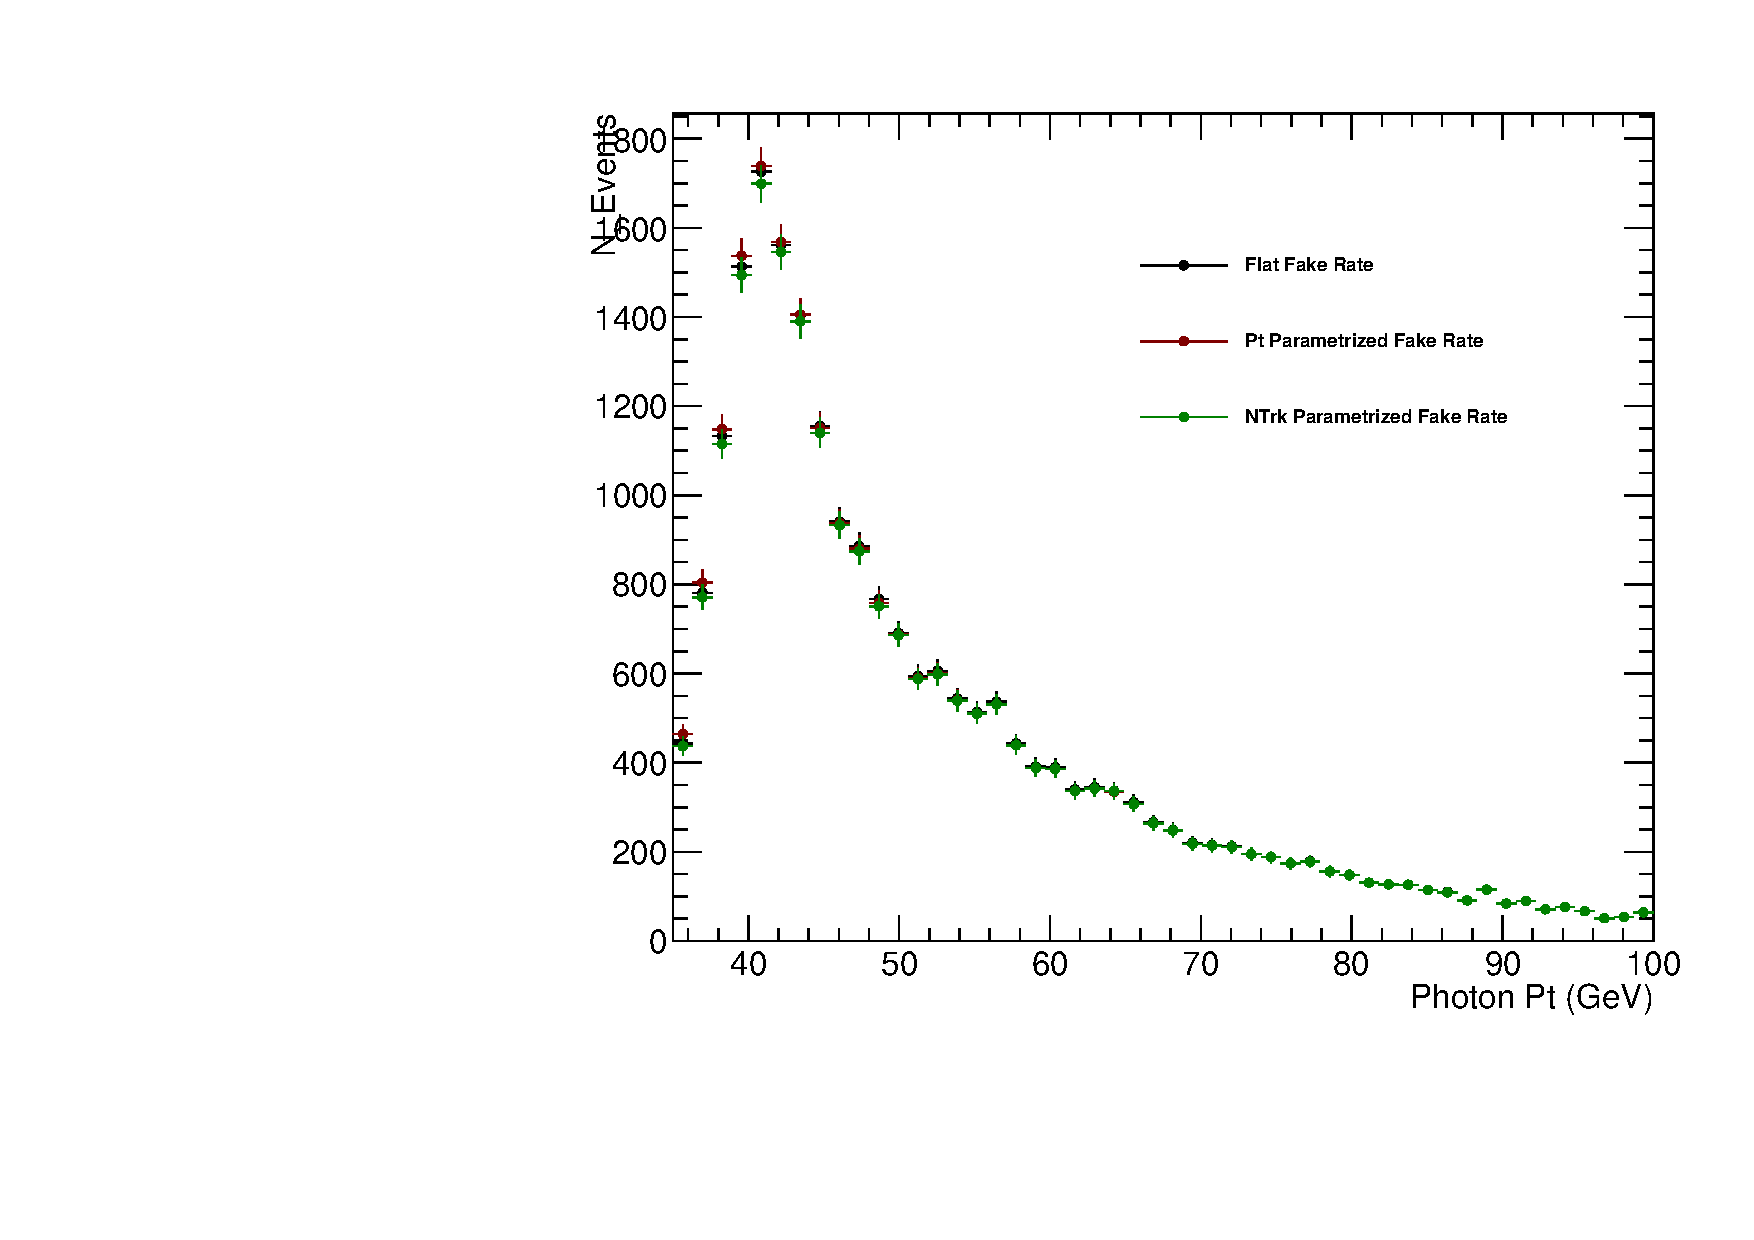
\includegraphics[width=0.45\textwidth]{efake_figs/CS_param_pt.pdf}}
  {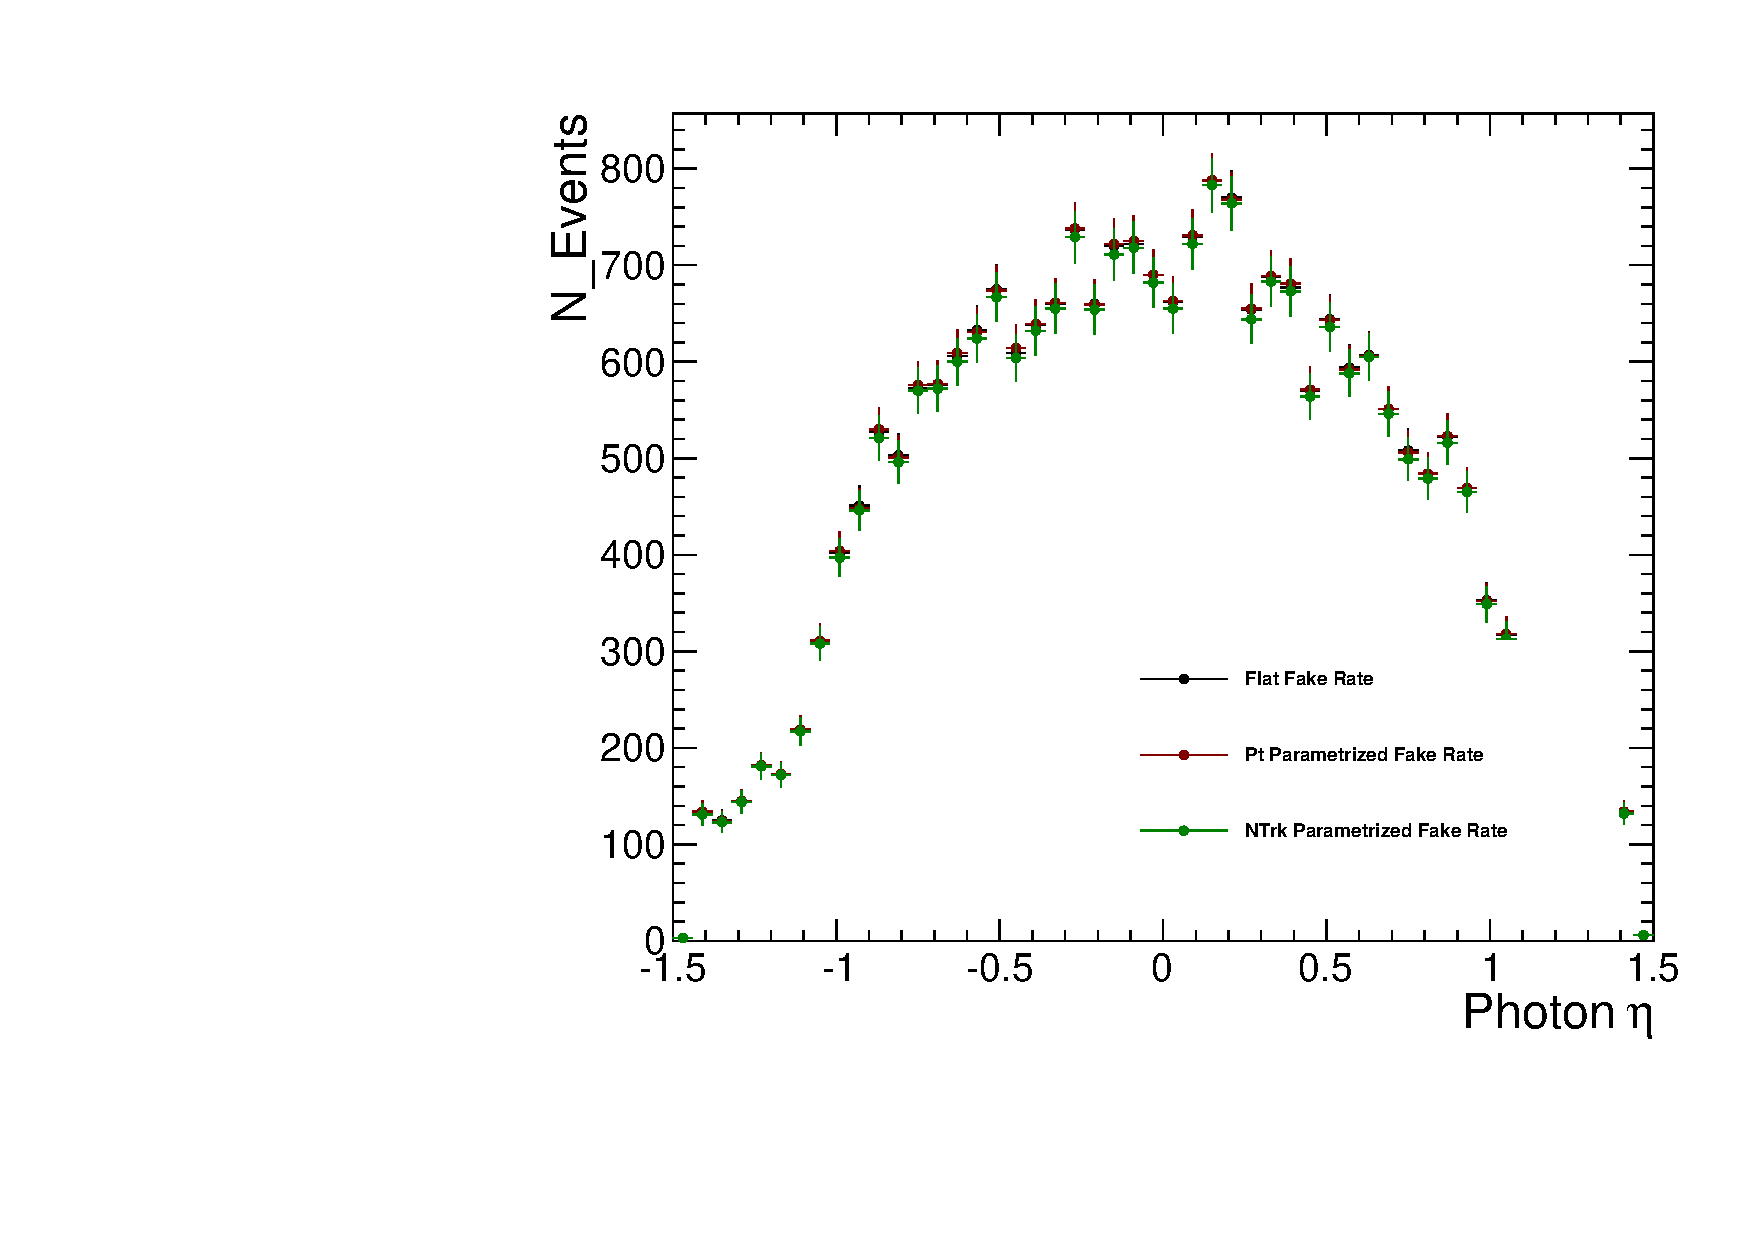
\includegraphics[width=0.45\textwidth]{efake_figs/CS_param_eta.pdf}}
\\
  {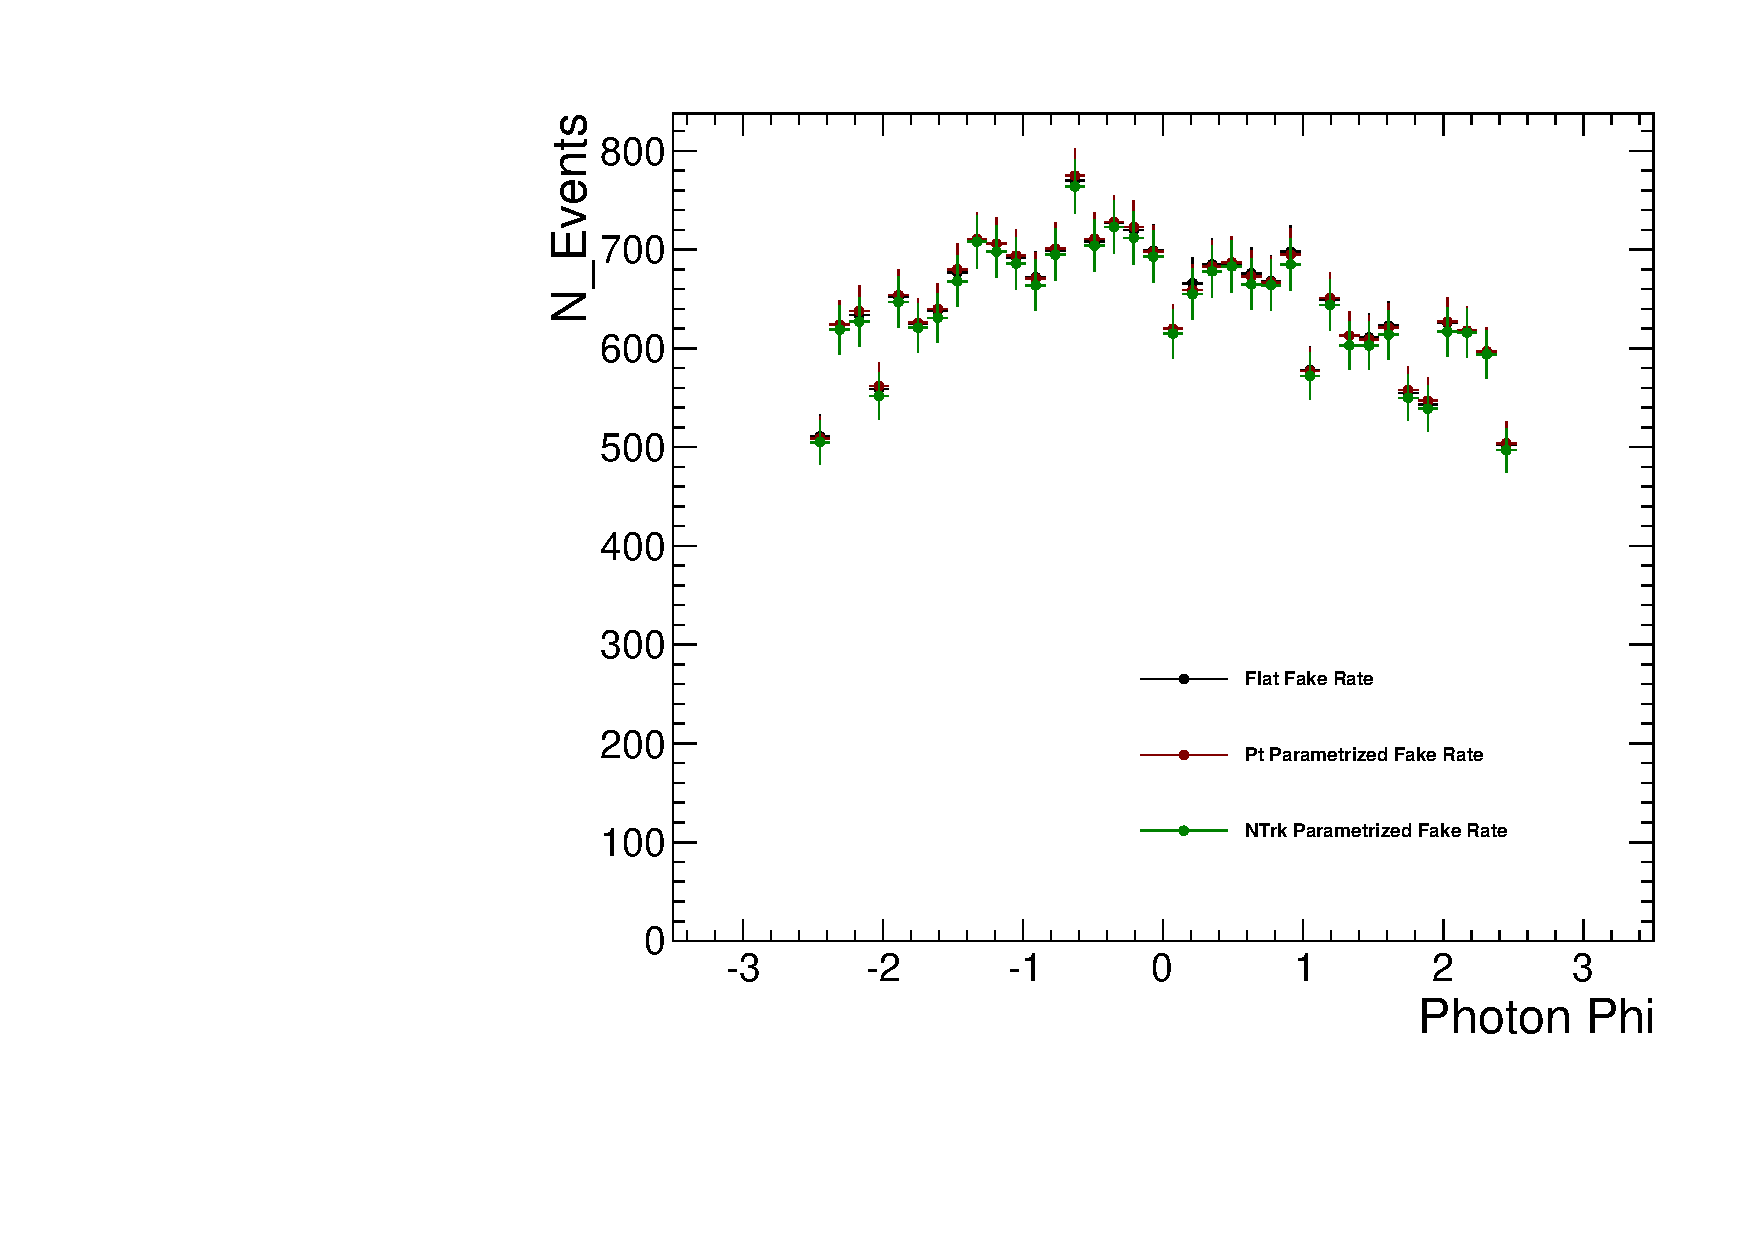
\includegraphics[width=0.45\textwidth]{efake_figs/CS_param_phi.pdf}}
\caption{Control sample distribution of photon $p_T$, $\eta$ and $\phi$.}
\label{CS_params}
\end{center}
\end{figure}

\subsubsection{Closure Test for Electron $\rightarrow$ Photon Fake Rate Measurment}

As a closure test, we compare the generator-level fake rate to the fake rate as calculated by the method described above on MC (the reco-level fake rate) and check that they agree.
%To make sure the method makes sense, we have to test whether or not it closes on Monte Carlo. That means that we have to compare the generator-level fake rate to the method fake rate on Monte Carlo and make sure that they agree. 
For that, we used the Drell-Yan sample.

The generator-level fake rate is defined as:

\begin{eqnarray}
F_{gen} = \frac{\textrm{\#Medium ID Photons \&\& Matched to Gen Electrons \&\& Pass the PSV}}{\textrm{\#Medium ID Photons \&\& Matched to Gen Electrons}}. \label{gen_fake}
\end{eqnarray}

Here, the Medium photon ID is the one used on the analysis, including all the shower shape cuts to remove spikes and other contributions.

We compare the results of the two measurements, generator-level and reco-level, on the plots in Figure \ref{closure_old}.

\begin{figure}[H]
\begin{center}
{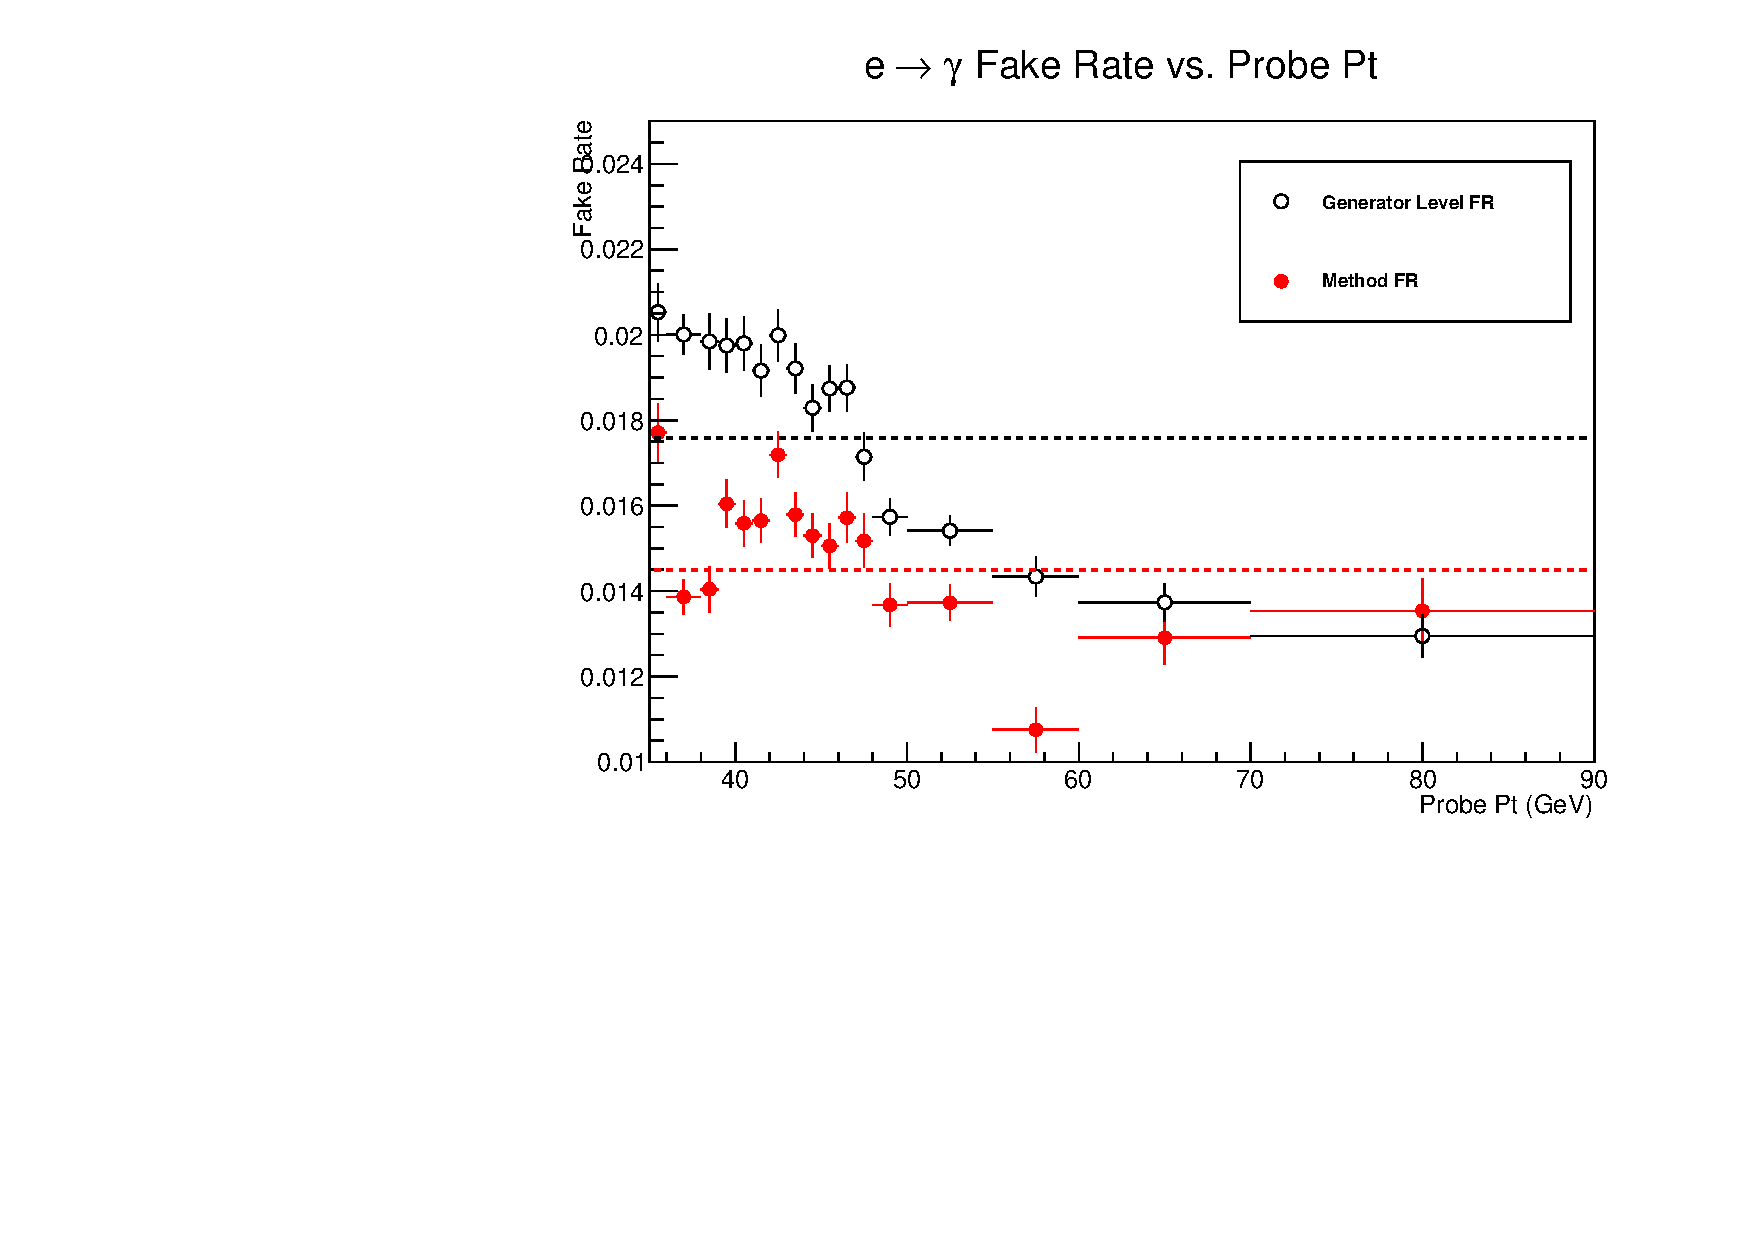
\includegraphics[width=0.45\textwidth]{efake_figs/closure_old_pt.pdf}}
{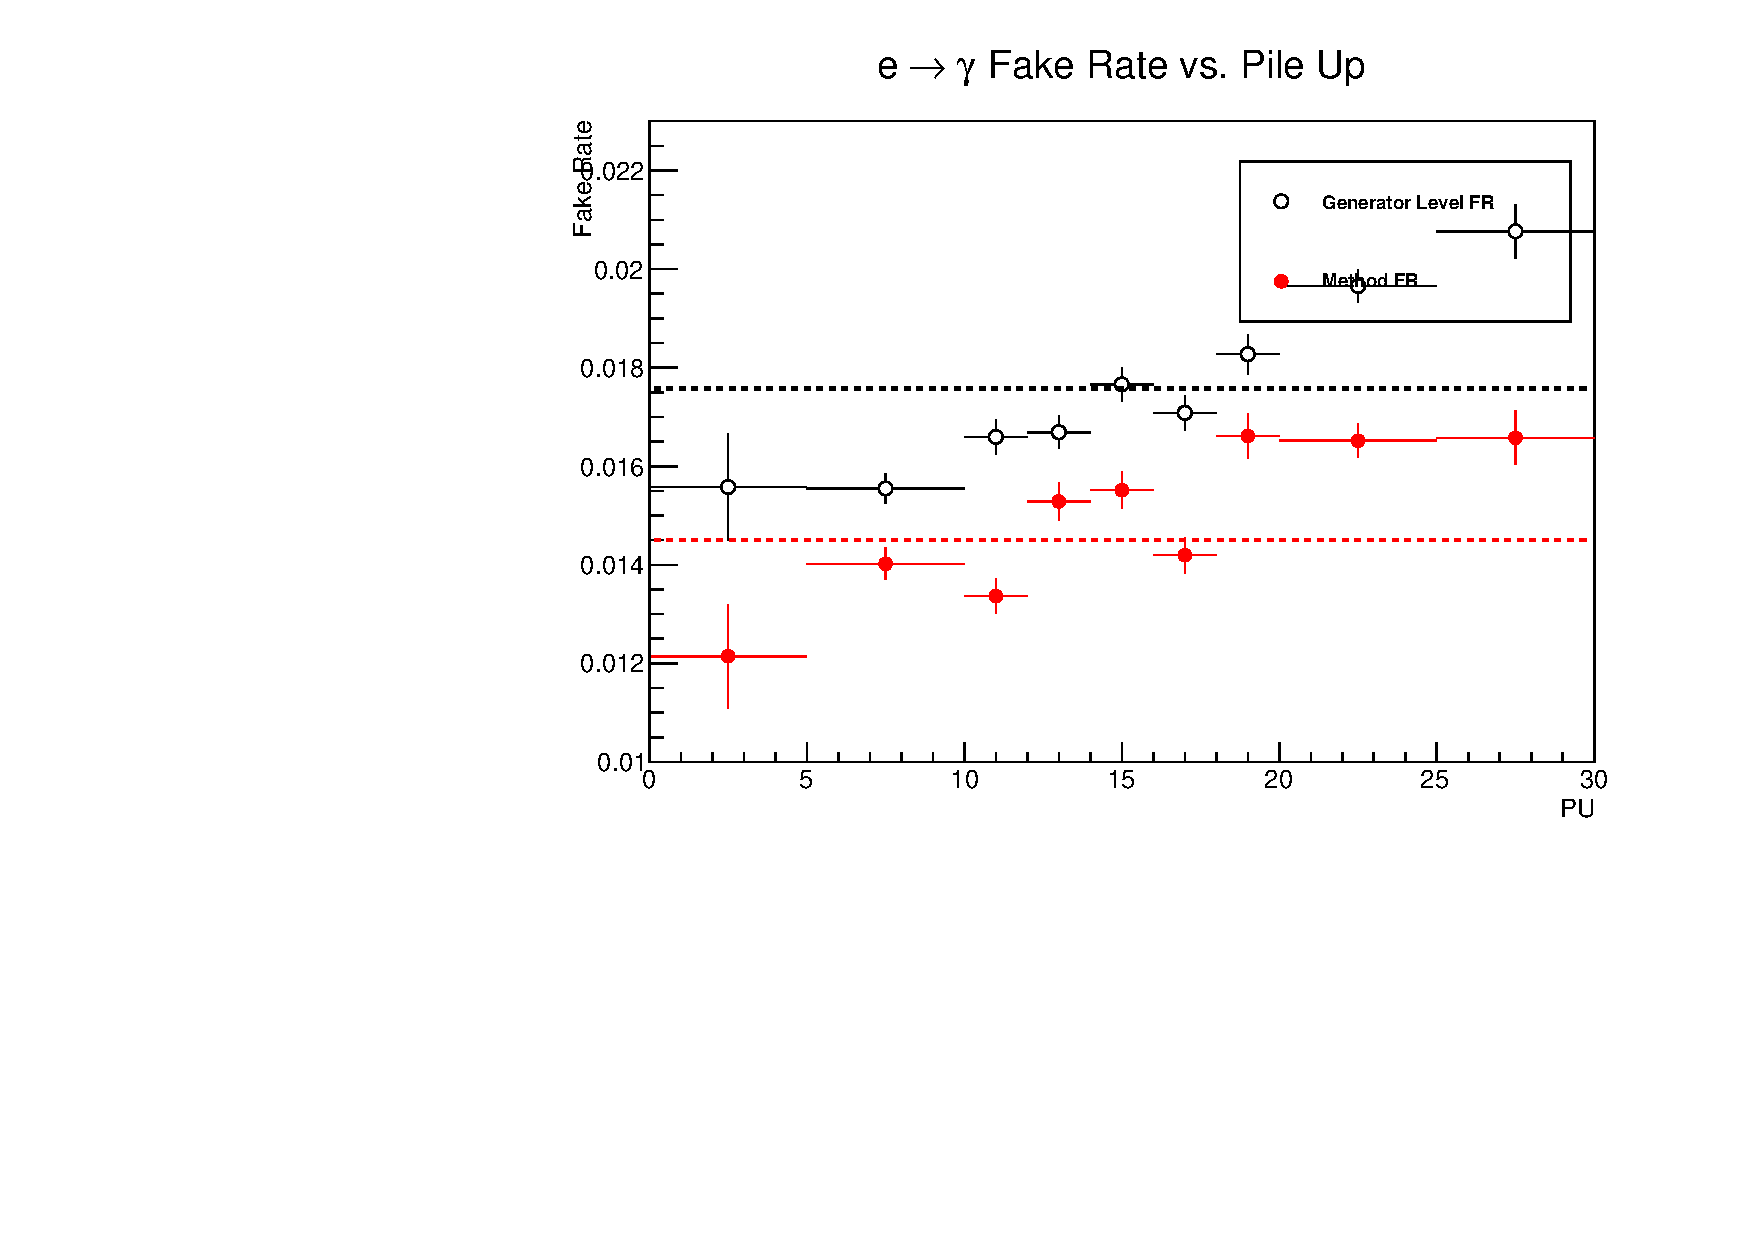
\includegraphics[width=0.45\textwidth]{efake_figs/closure_old_pu.pdf}}
\\
{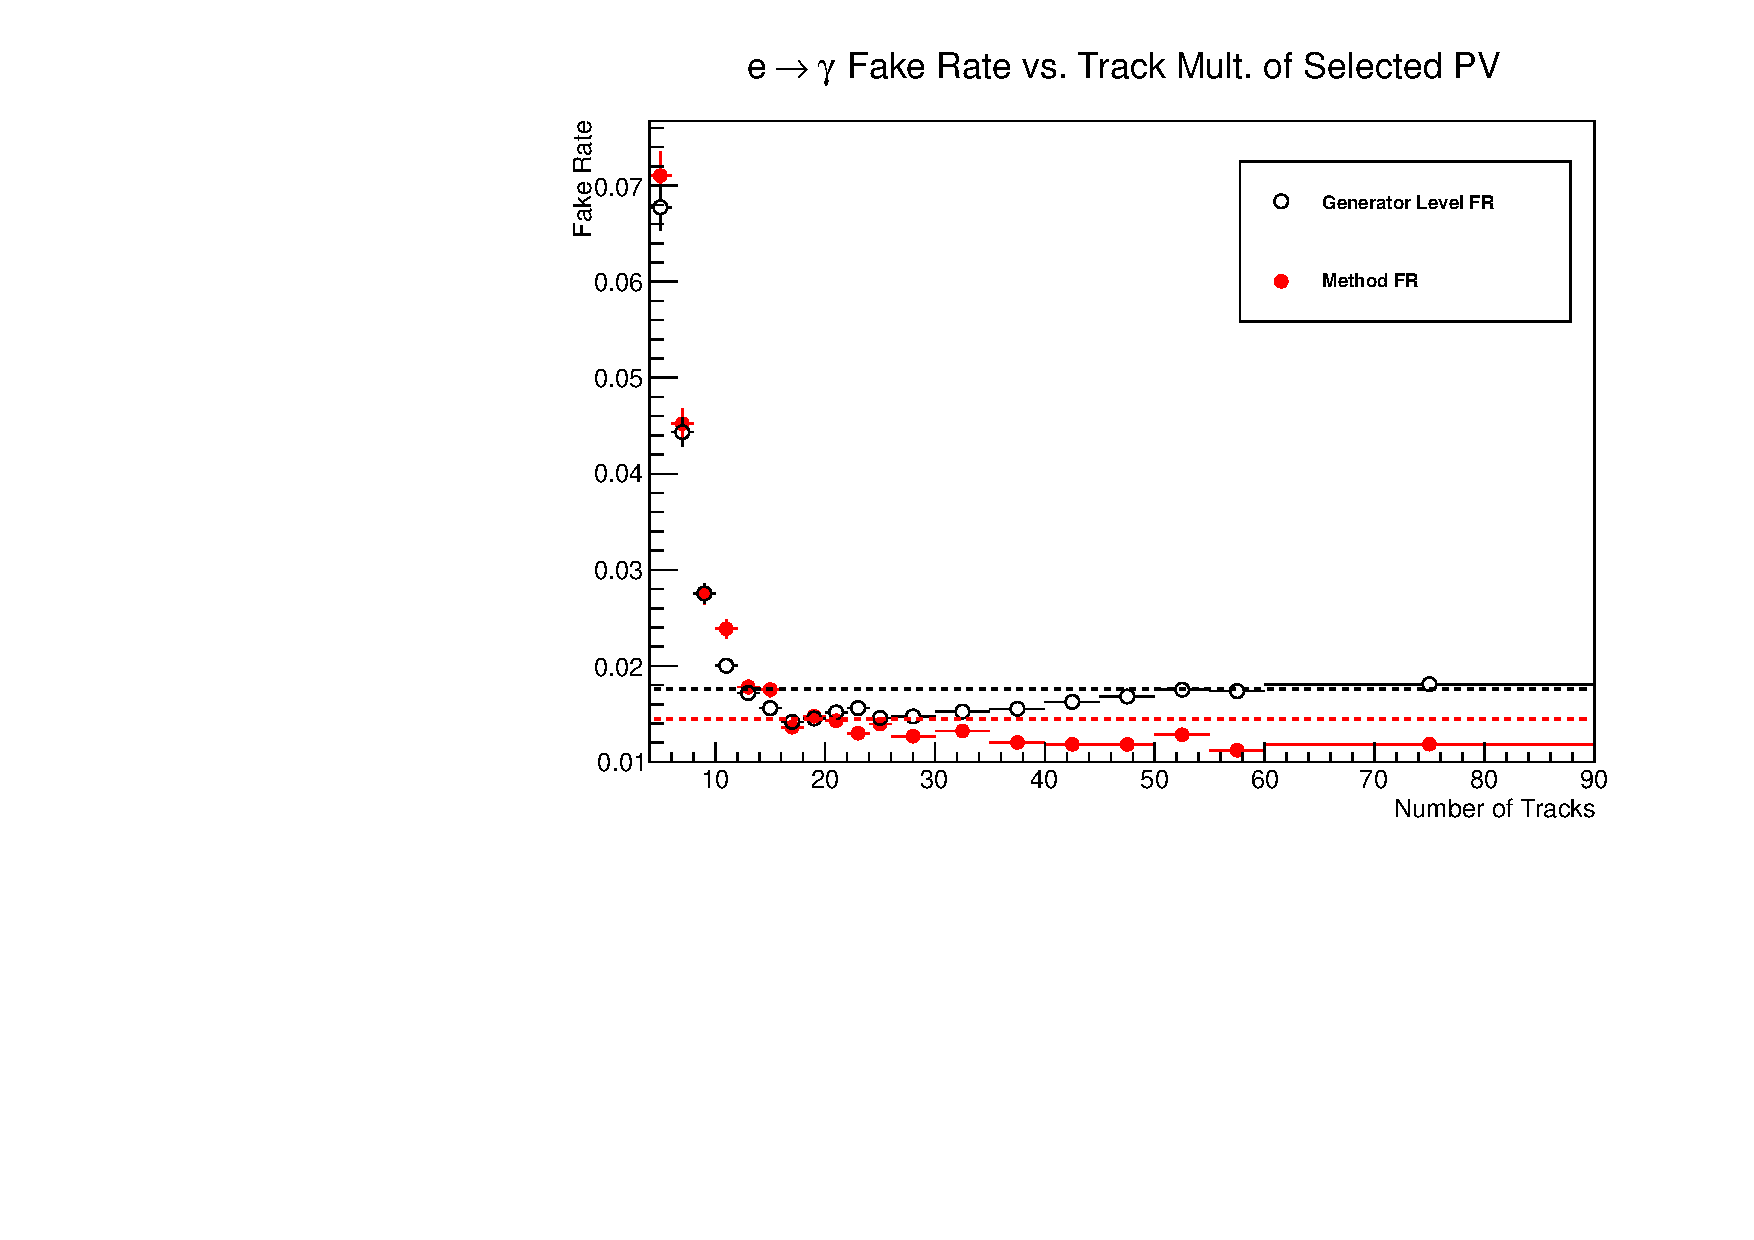
\includegraphics[width=0.45\textwidth]{efake_figs/closure_old_trk.pdf}}
\caption{Closure test in probe $p_T$,number of reconstructeed primary vertices and track multiplicity .}
\label{closure_old}
\end{center}
\end{figure}
%
%\begin{figure}[H]
%\begin{center}
%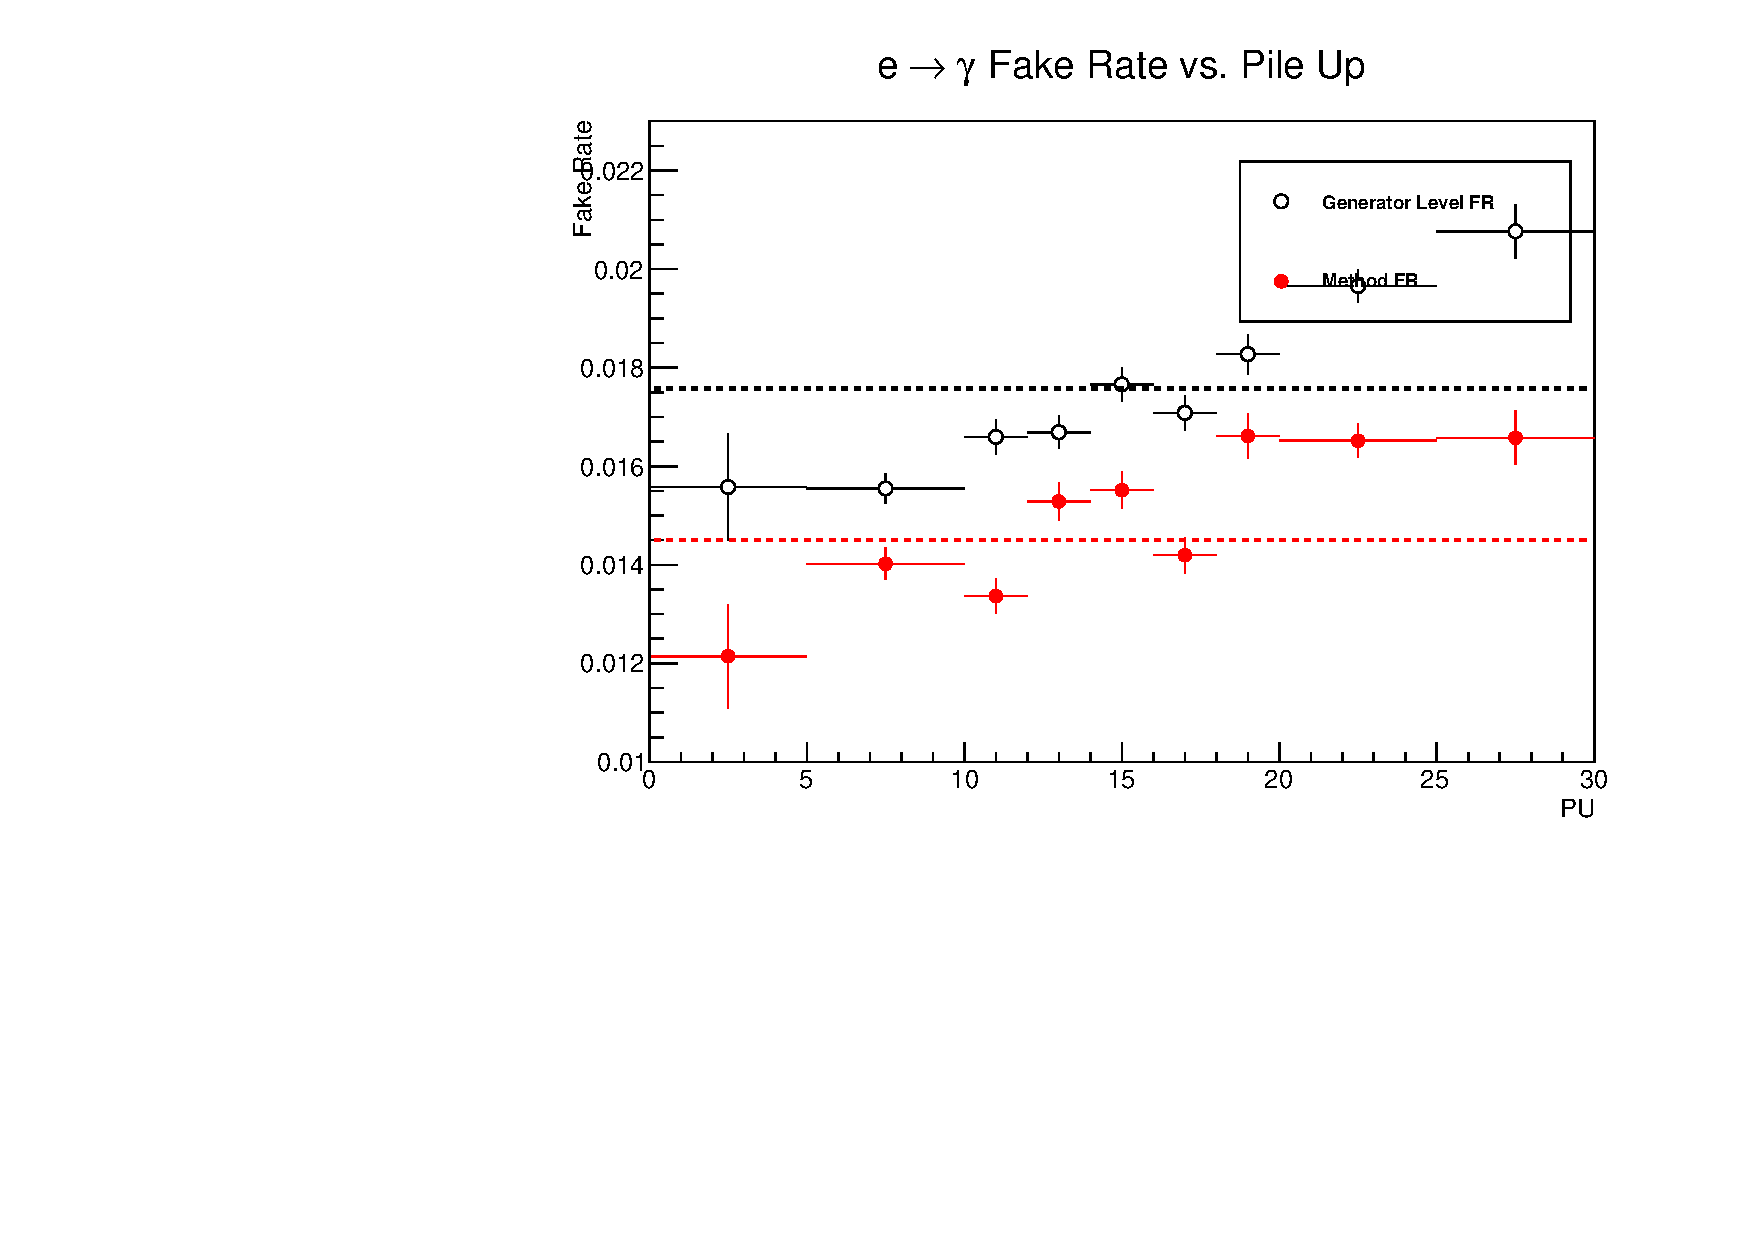
\includegraphics[scale=0.5]{efake_figs/closure_old_pu.pdf}
%\caption{Closure test in number of reconstructeed primary vertices.}
%\label{closure_old_pu}
%\end{center}
%\end{figure}

%\begin{figure}[H]
%\begin{center}
%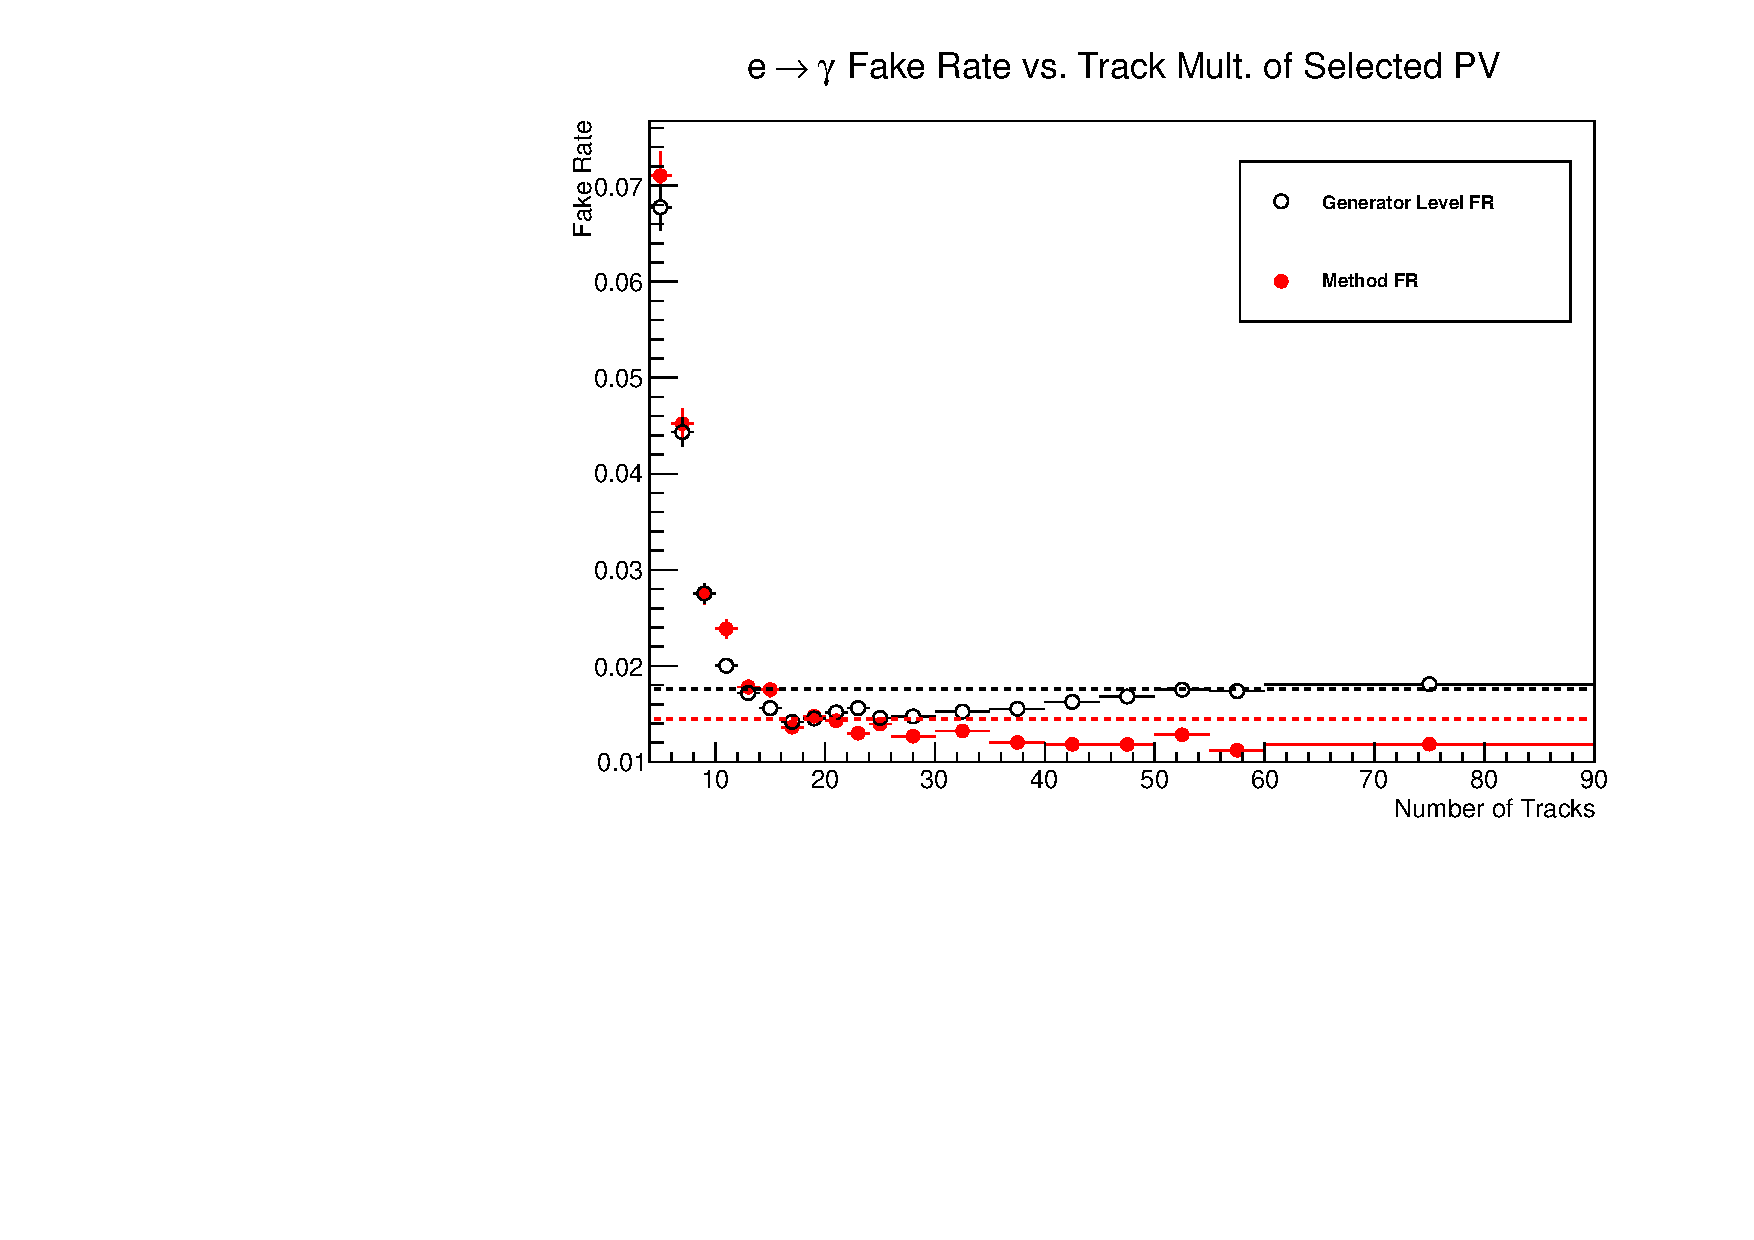
\includegraphics[scale=0.5]{efake_figs/closure_old_trk.pdf}
%\caption{Closure test in track multiplicity.}
%\label{closure_old_ntrk}
%\end{center}
%\end{figure}

The lines represent the fake rate results from the flat assumption. For the generator-level fake rate, that is just the ratio on equation \ref{gen_fake} on all events, while the parametrized fake rate is the ratio in each bin. As shown, there is a significant discrepancy between the two measurements. With those results, we can only say that the method is closed within 20\%. The 20\% number comes from the difference between the flat fake rates on generator-level and reco-level results.

We investigated the cause of this result and noticed that it comes about because of a "hidden" primary vertex matching on the tag-and-probe method. When using the tag and probe for electrons as tag and photons as probe, the photon ends up being matched to the hardest primary vertex because the electron, in the electron ID requirements, is indeed matched. When we require the invariant mass of the pair to be close to the $Z$ peak, the electron PV matching is indirectly passed to the probe photon, since they must come from the same source. This requirement does not exist on the gen-level fake rate, which is basically a counting experiment.

The importance of the PV matching requirement comes about because of the nature of the DY$\to ee$ process. Since it is a low multiplicity process, i.e., there will not be many objects naturally from the hard scatter process, the $Z$ might not come from the hardest reconstructed primary vertex of the event. Therefore, when that happens, we measure the fake rate from a  primary vertex that is not the hardest and, therefore, has fewer tracks than the primary vertex assumed. Since we know that the fake rate increases sharply when there are few tracks in the primary vertex, that explains why, in plot \ref{closure_old}, there is an increase in higher values of NTrack - those are actually hard scatter events with few tracks that were mistakenly matched to the hardest PV.

To overcome these problems, we match the gen-level particles used for the gen-level fake rate to the hardest reconstructed primary vertex with the following cuts (from the muon ID POG recommendations):

\begin{itemize}
\item $Dz < 0.5$;
\item $Dxy < 0.2$.
\end{itemize}

These variables are obtained directly from methods of the RECO::Candidate class inherited by the RECO::GenParticle.
With that, we have the plots on Figure \ref{closure_all}.

\begin{figure}[H]
\begin{center}
{\label{closure_pt}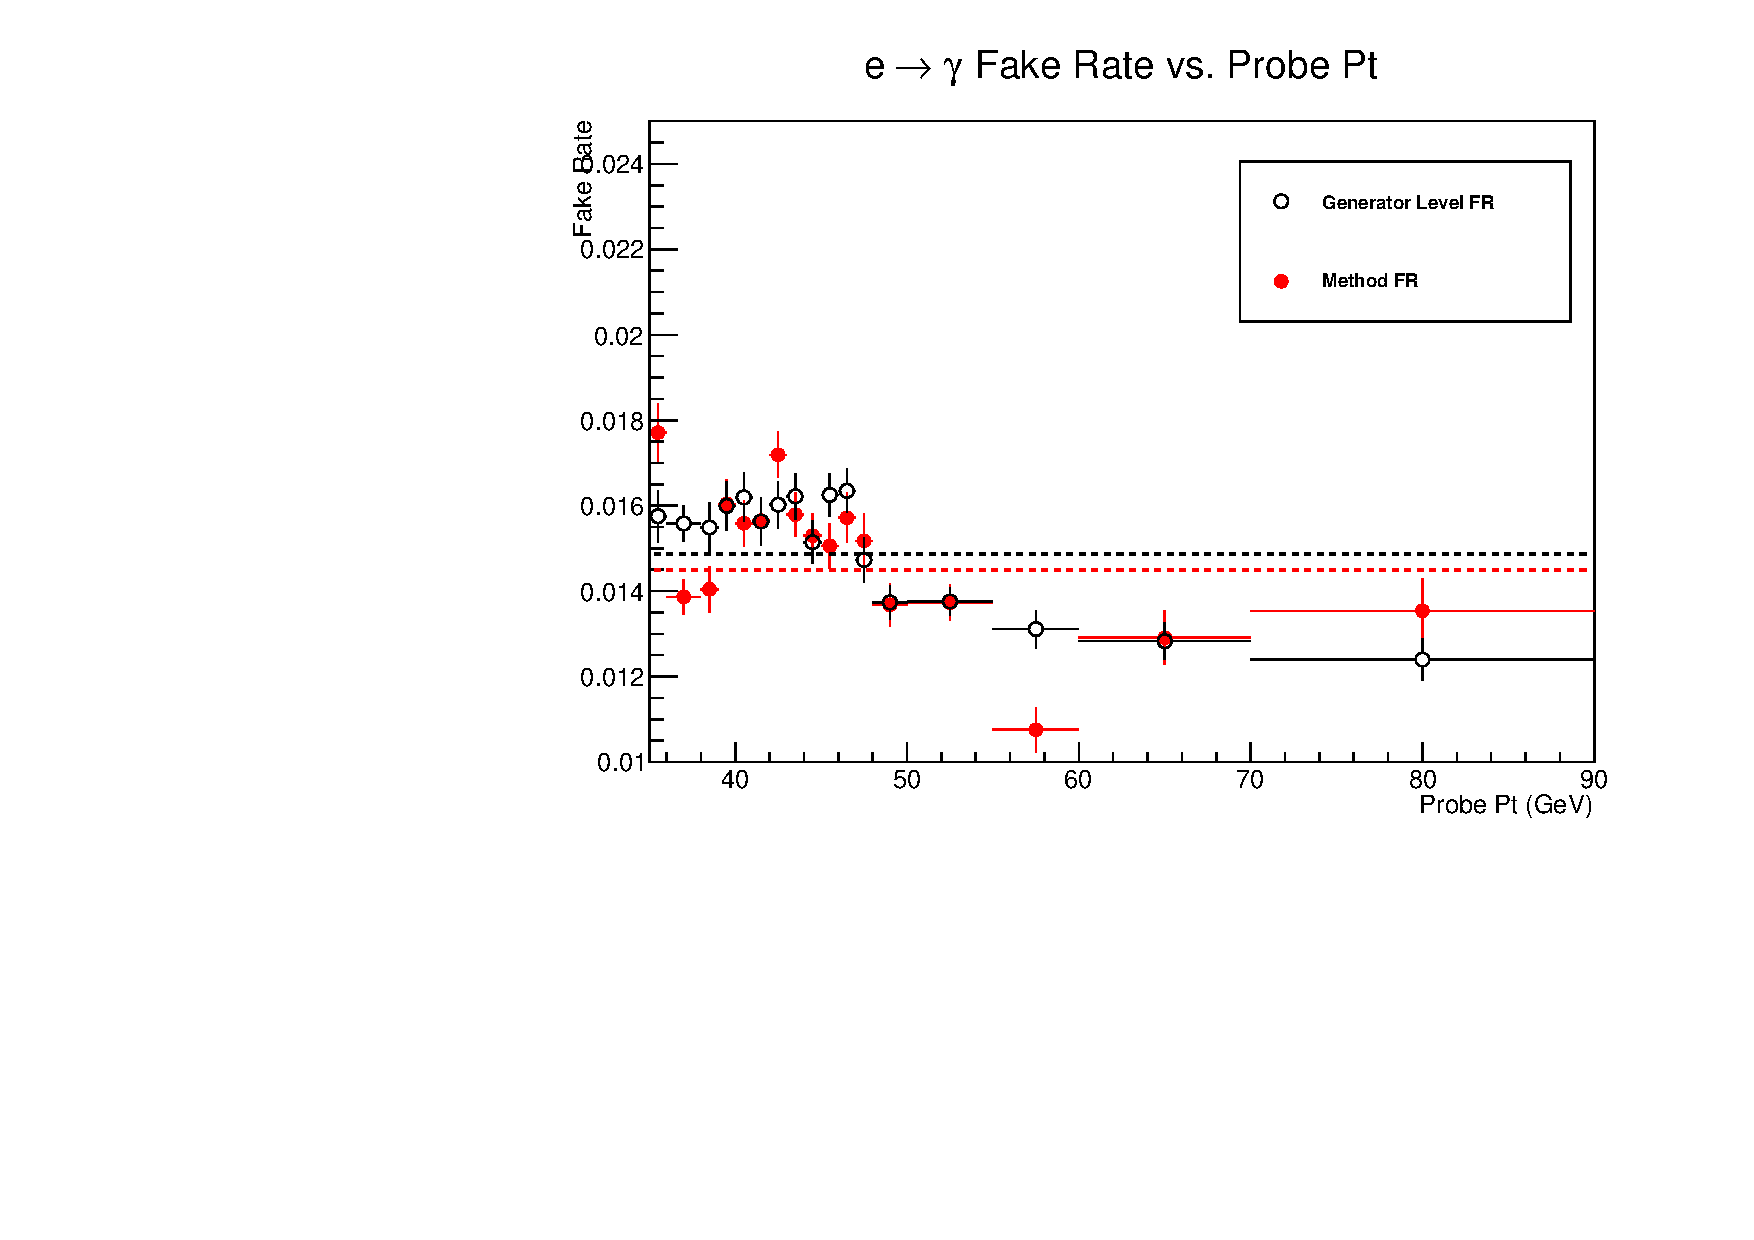
\includegraphics[width=0.45\textwidth]{efake_figs/closure_pt.pdf}}
{\label{closure_pu}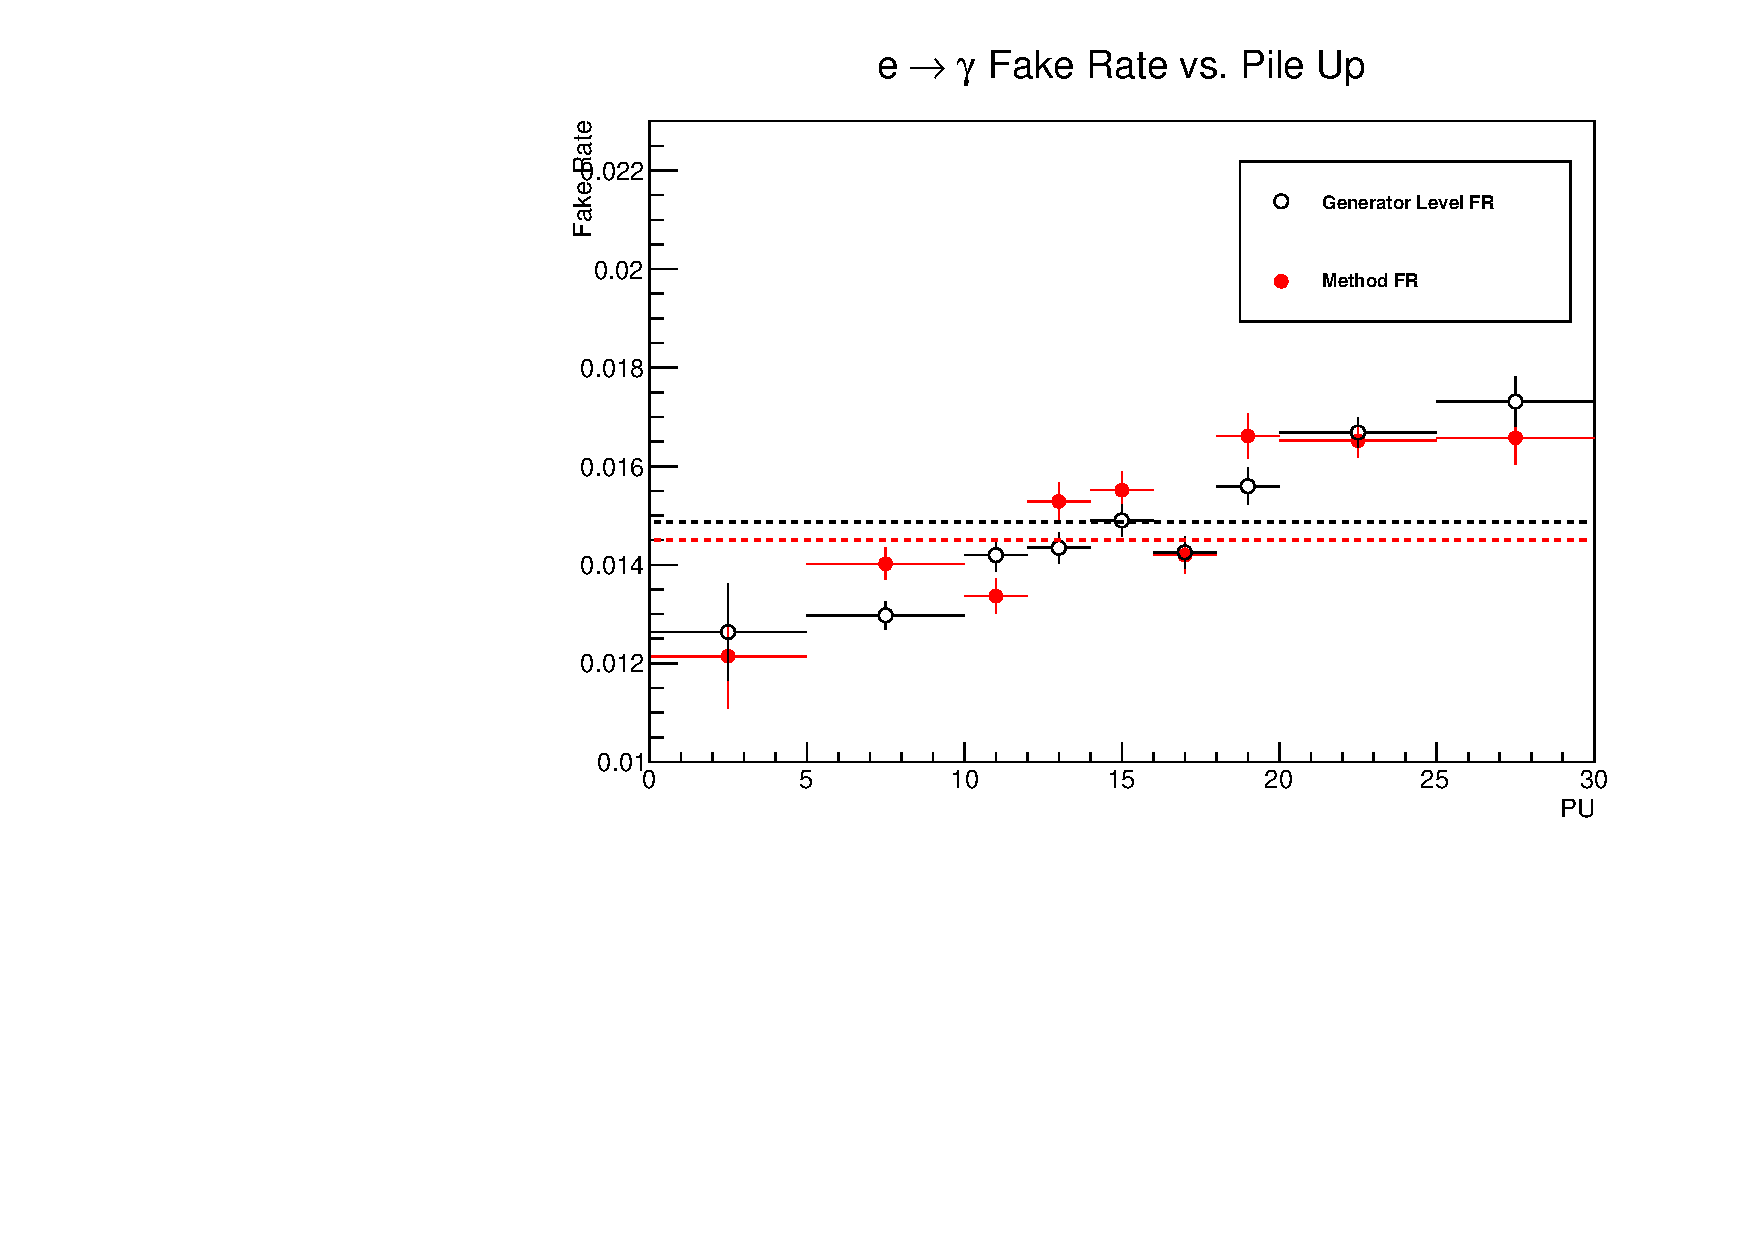
\includegraphics[width=0.45\textwidth]{efake_figs/closure_pu.pdf}}
\\
{\label{closure_ntrk}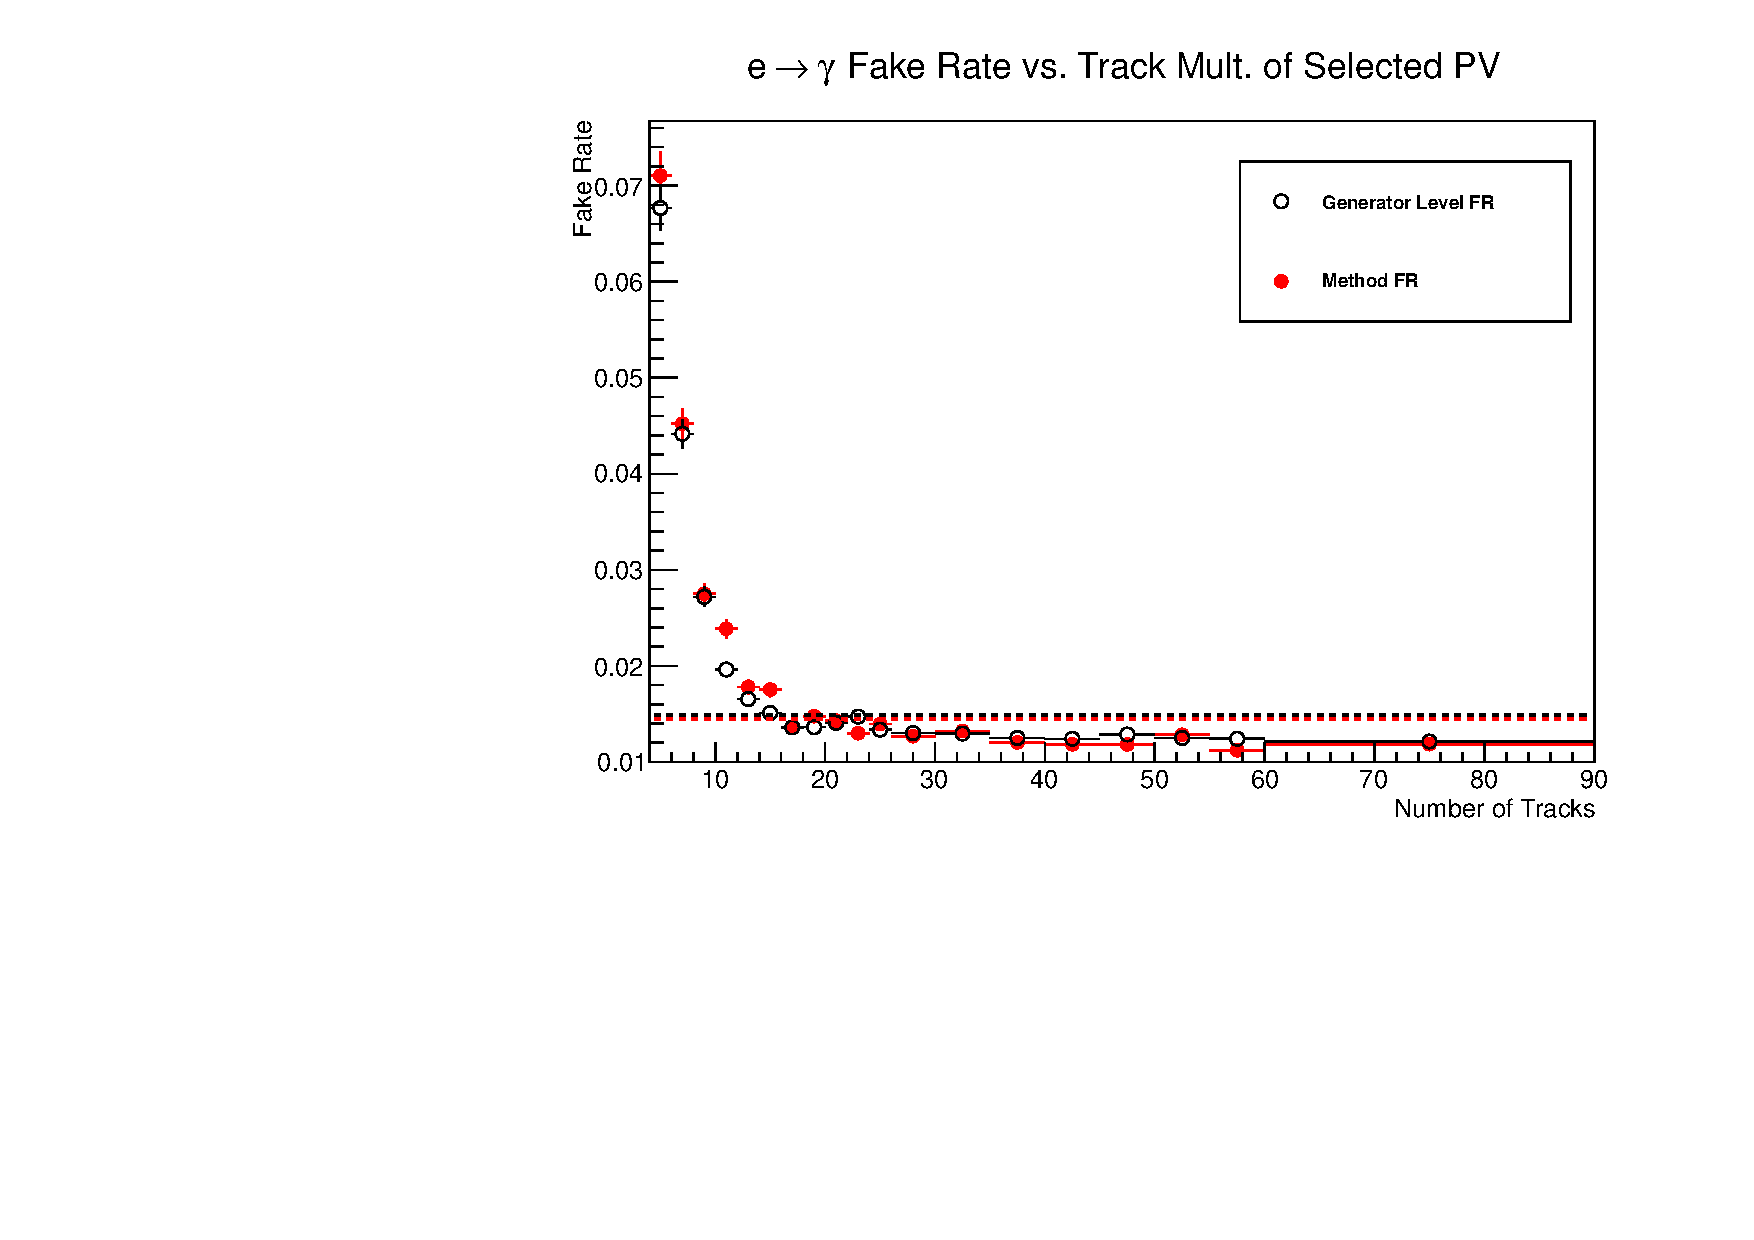
\includegraphics[width=0.45\textwidth]{efake_figs/closure_trk.pdf}}
\caption{PV matched closure test in probe $p_T$,number of reconstructeed primary vertices and track multiplicity}
\label{closure_all}
\end{center}
\end{figure}

%\begin{figure}[H]
%\begin{center}
%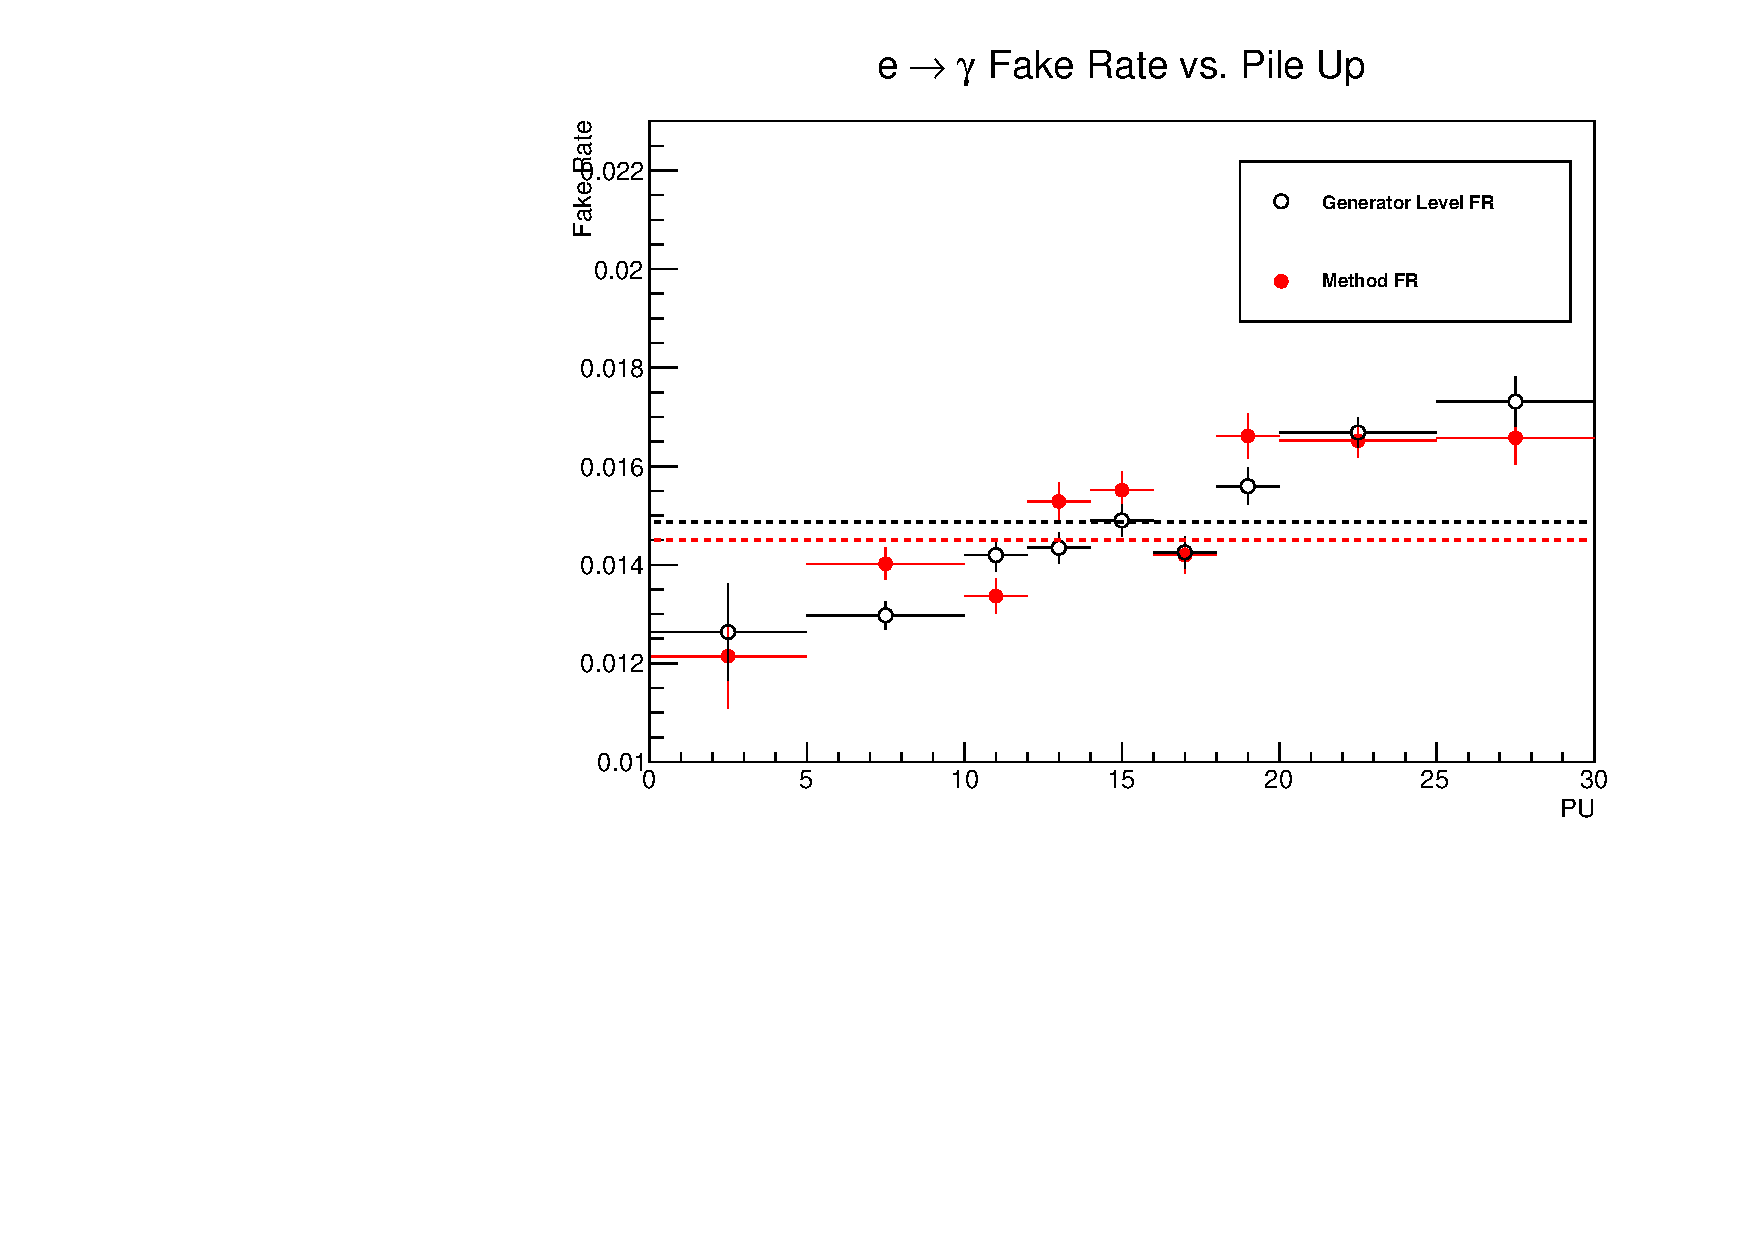
\includegraphics[scale=0.5]{efake_figs/closure_pu.pdf}
%\caption{PV matched closure test in number of reconstructeed primary vertices.}
%\label{closure_pu}
%\end{center}
%\end{figure}

%\begin{figure}[H]
%\begin{center}
%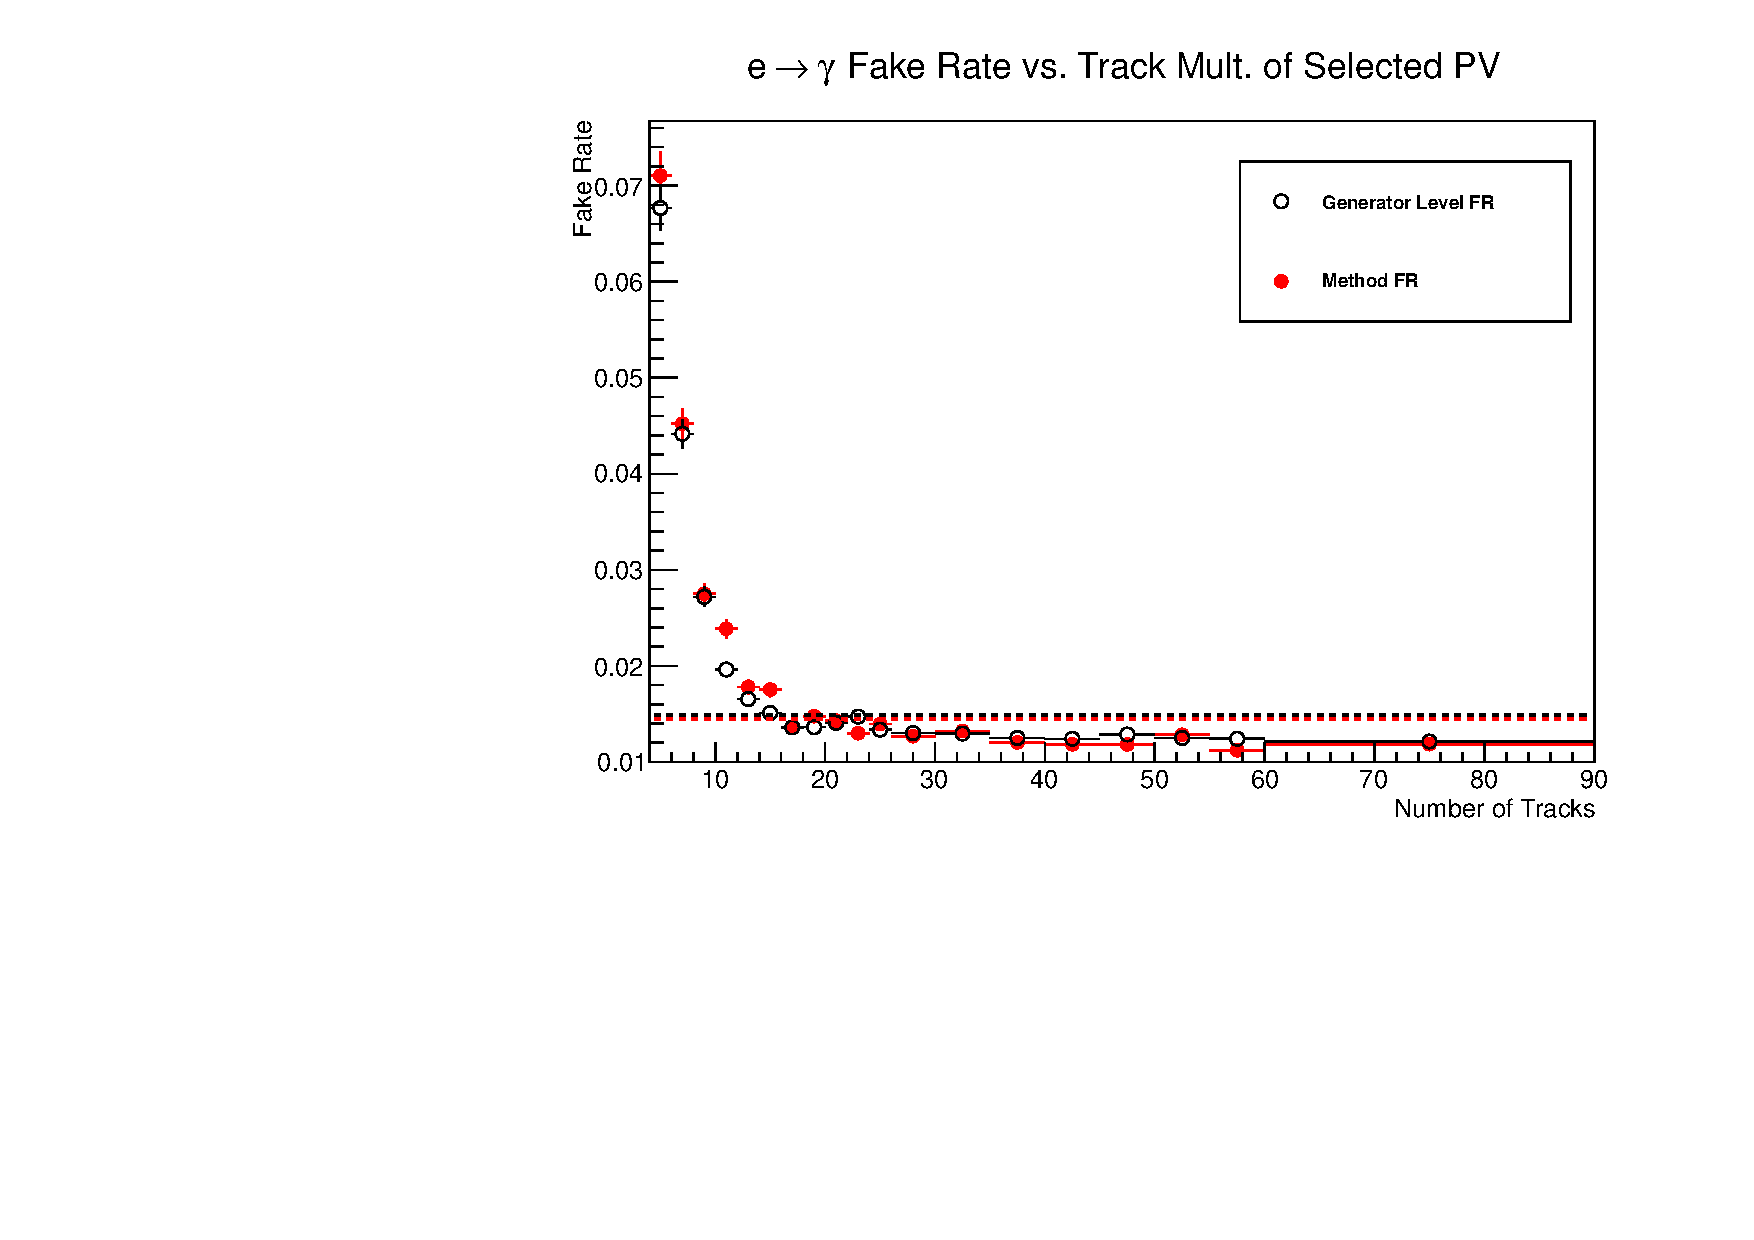
\includegraphics[scale=0.5]{efake_figs/closure_trk.pdf}
%\caption{PV matched closure test in track multiplicity.}
%\label{closure_ntrk}
%\end{center}
%\end{figure}

We can see that the agreement between the gen-level and reco-level fake rates improves and the method closes within 4\%.

\subsubsection{Systematic Uncertainty on the Electron $\rightarrow$ Photon Fake Rate Measurement}
Two of the main systematic errors have been discussed in the previous section:

\begin{itemize}
\item The flat assumption systematic error is found to be 5\% on the number of events;
\item The closure test systematic is found to be 4\% on the value of the fake rate.
\end{itemize}

The remaining systematic uncertainty is related to the background estimation Fig.~\ref{Zeall}, i.e. the choice of the functional form to represent the backgroun composition. Two choices were made for that estimation: a simple decaying exponential and the RooCMSShape. Looking at the full mass spectrum of the invariant mass, without parametrization, the amount of expected background is much smaller than the number of signal events. Because of that, we don't expect the fake rate to be very dependent on the functional shape of the background. Indeed, the difference in the calculated fake rate for the two functions is about 4\%.

These systematic errors are assumed independent and should be added as such in the final number for the fake rate. They are, however, very small compared to the other sources of systematic errors in the analysis.


\subsection{Non-Collision Backgrounds}
\label{sec:noncollision}

We estimate the rate of non-collision backgrounds which produce prompt photons using the ECAL timing variables for EM cluster. This estimate includes the contributions from ECAL “spikes”, as well as beam halo. To estimate these contribution we form crystal seed timing distributions of each background component i.e., spikes, beam halo and then fitted them to the candidate seed time distribution without shower shape or timing cuts to estimate how much each of these background contribute in the prompt region (  $|t_{seed} | < 3 $ns).

 The various templates are formed in the following way: 
    
\begin{itemize}
\item {\bf Candidate sample templates}: To construct the template for the candidate sample we apply cuts similar to our analysis cuts but with relaxed the shower shape variables and without offline R9 selection. We do not apply any fake E/T rejection cuts to increase the statistics in our templates. The distribution can be seen in Fig.\ref{fig:candidate}.
\item {\bf Prompt templates}: The templates for prompt events is made using the candidate sample in which the photon candidates are required to have a pixel seed match, as seen in Fig. ~\ref{fig:PromptTempl} .
\item {\bf Spikes templates}: The spike template is found by requiring one of the shower shape variables sihih 0.011 or sifif< 0.001 selection. These templates are shown in Fig. ~\ref{fig:SpikeTempl}.
\item {\bf Beam Halo templates}: The energy deposition from the beam halo muon could be reconstructed within the prompt window when the muon brems in the ECAL. To get the template of timing distributions of such objects, we apply similar cuts used for the candidate sample but require the MIP total energy to be greater than 4 GeV. The beam halo template is shown in Fig.~\ref{fig:beamhalo}. The MIP-tagging is a set of criteria developed in order to identify the passage of a beam halo muon across the acceptance of the ECAL. Crystals other than associated with EM shower  are identified along potential paths in a similar $\phi$ direction as of the seed crystal of EM shower, and then fitted with a straight line. The end results is the number of crystals associated along the selected trajectory, their total energy (MIP energy), and the $\chi^2$ of the fitted line. The beam hallo shower typicaly have more MIP energy than a true EM shower .
\end{itemize}



\begin{figure}[h]
\centering
{\label{fig:candidate}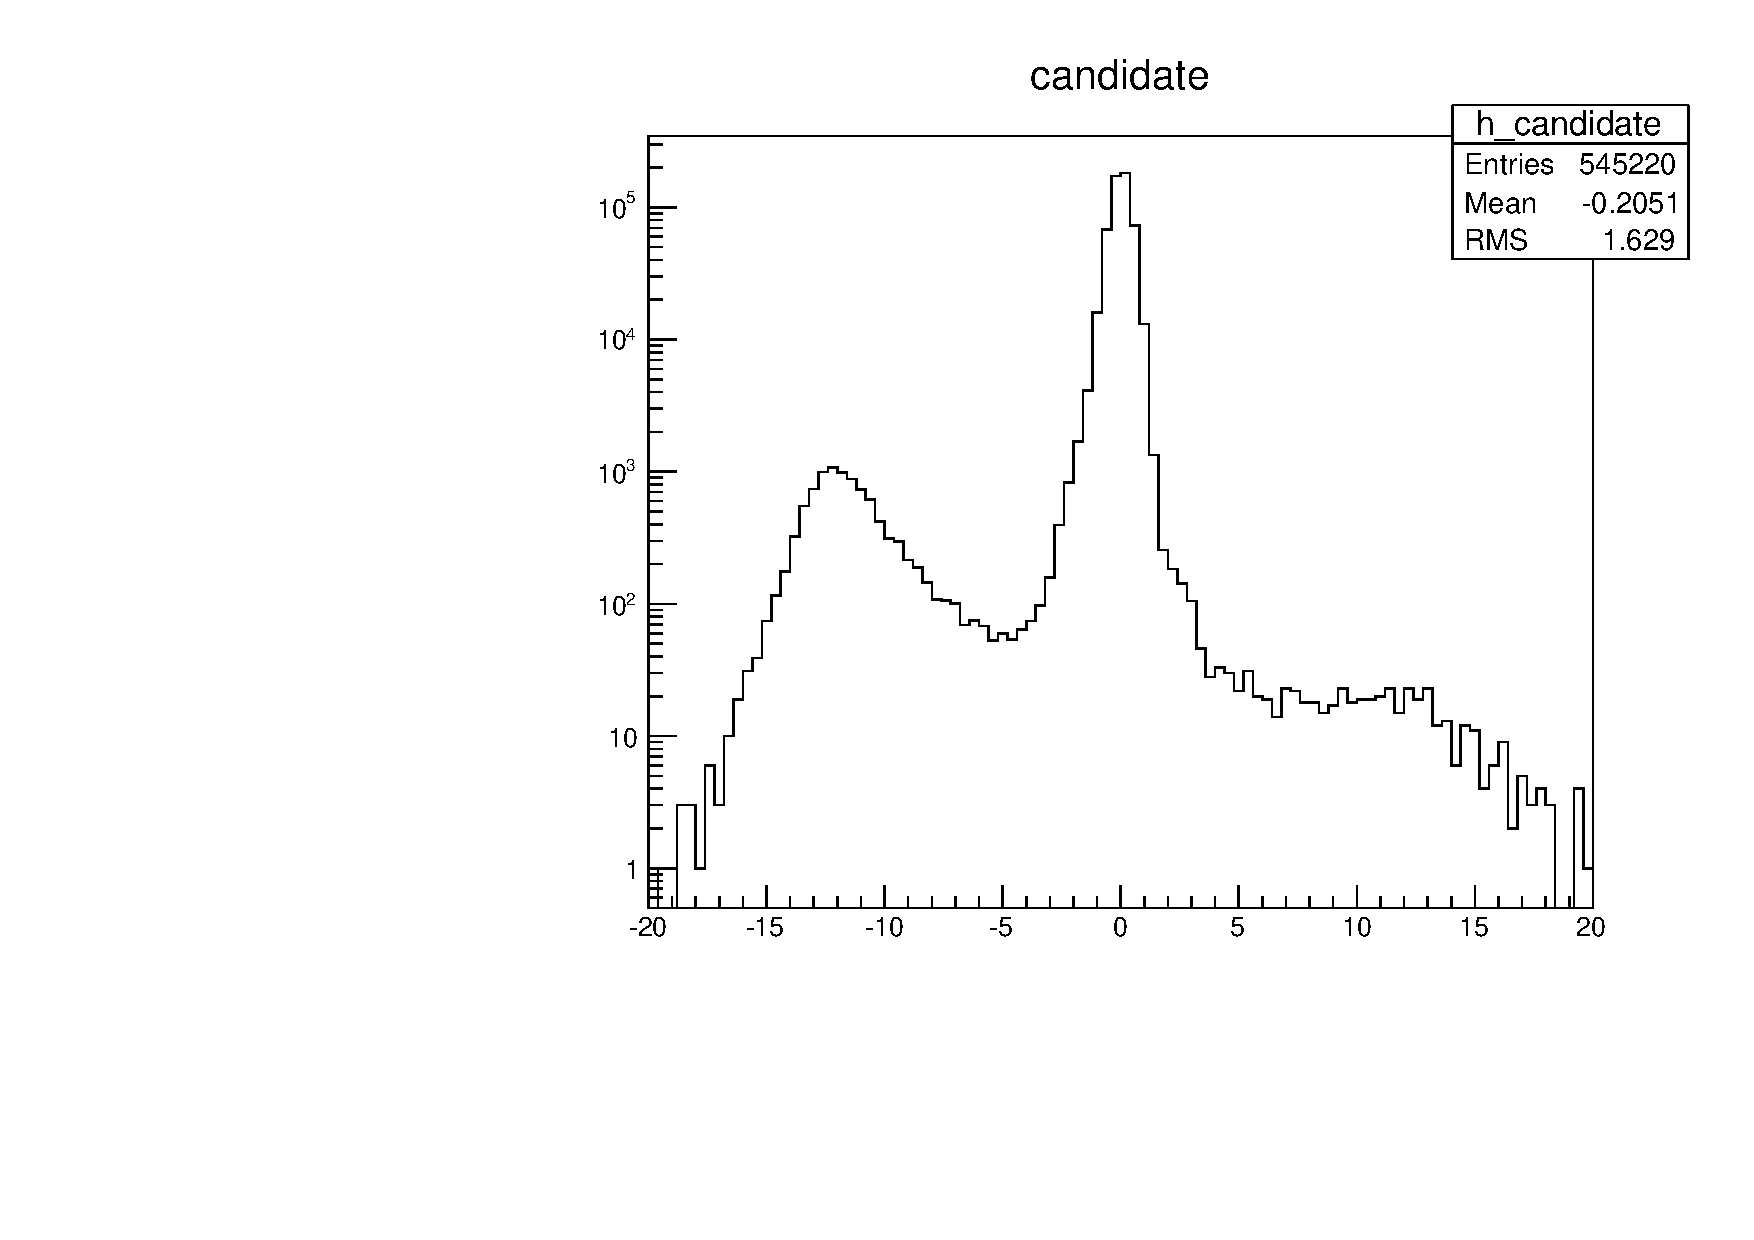
\includegraphics[width=0.45\textwidth]{analysis_figs/candidate_temp.pdf}}
{\label{fig:PromptTempl}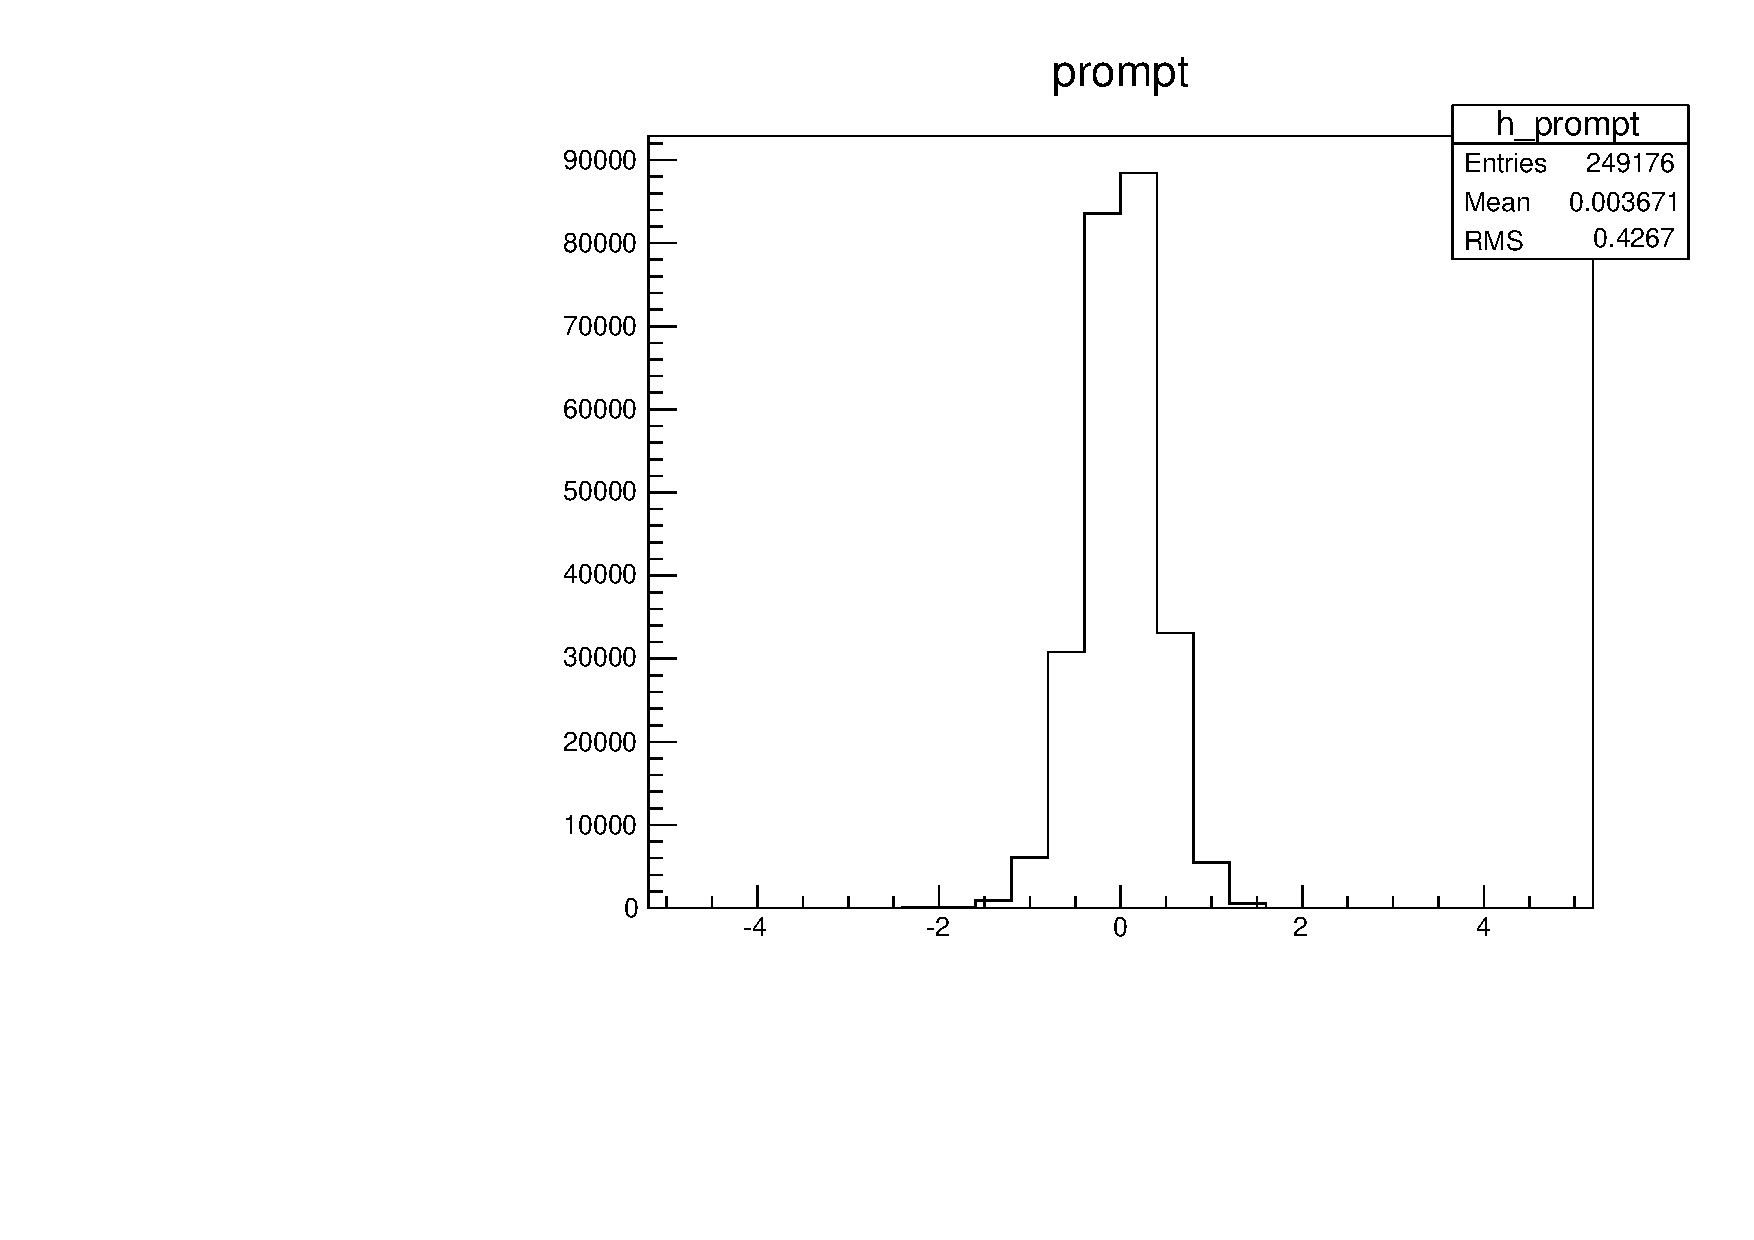
\includegraphics[width=0.45\textwidth]{analysis_figs/prompt.pdf}}
\caption{Seed time distribution (ns) for candidate events and prompt events.}
\end{figure}

\begin{figure}[h!]
\centering
{\label{fig:SpikeTempl}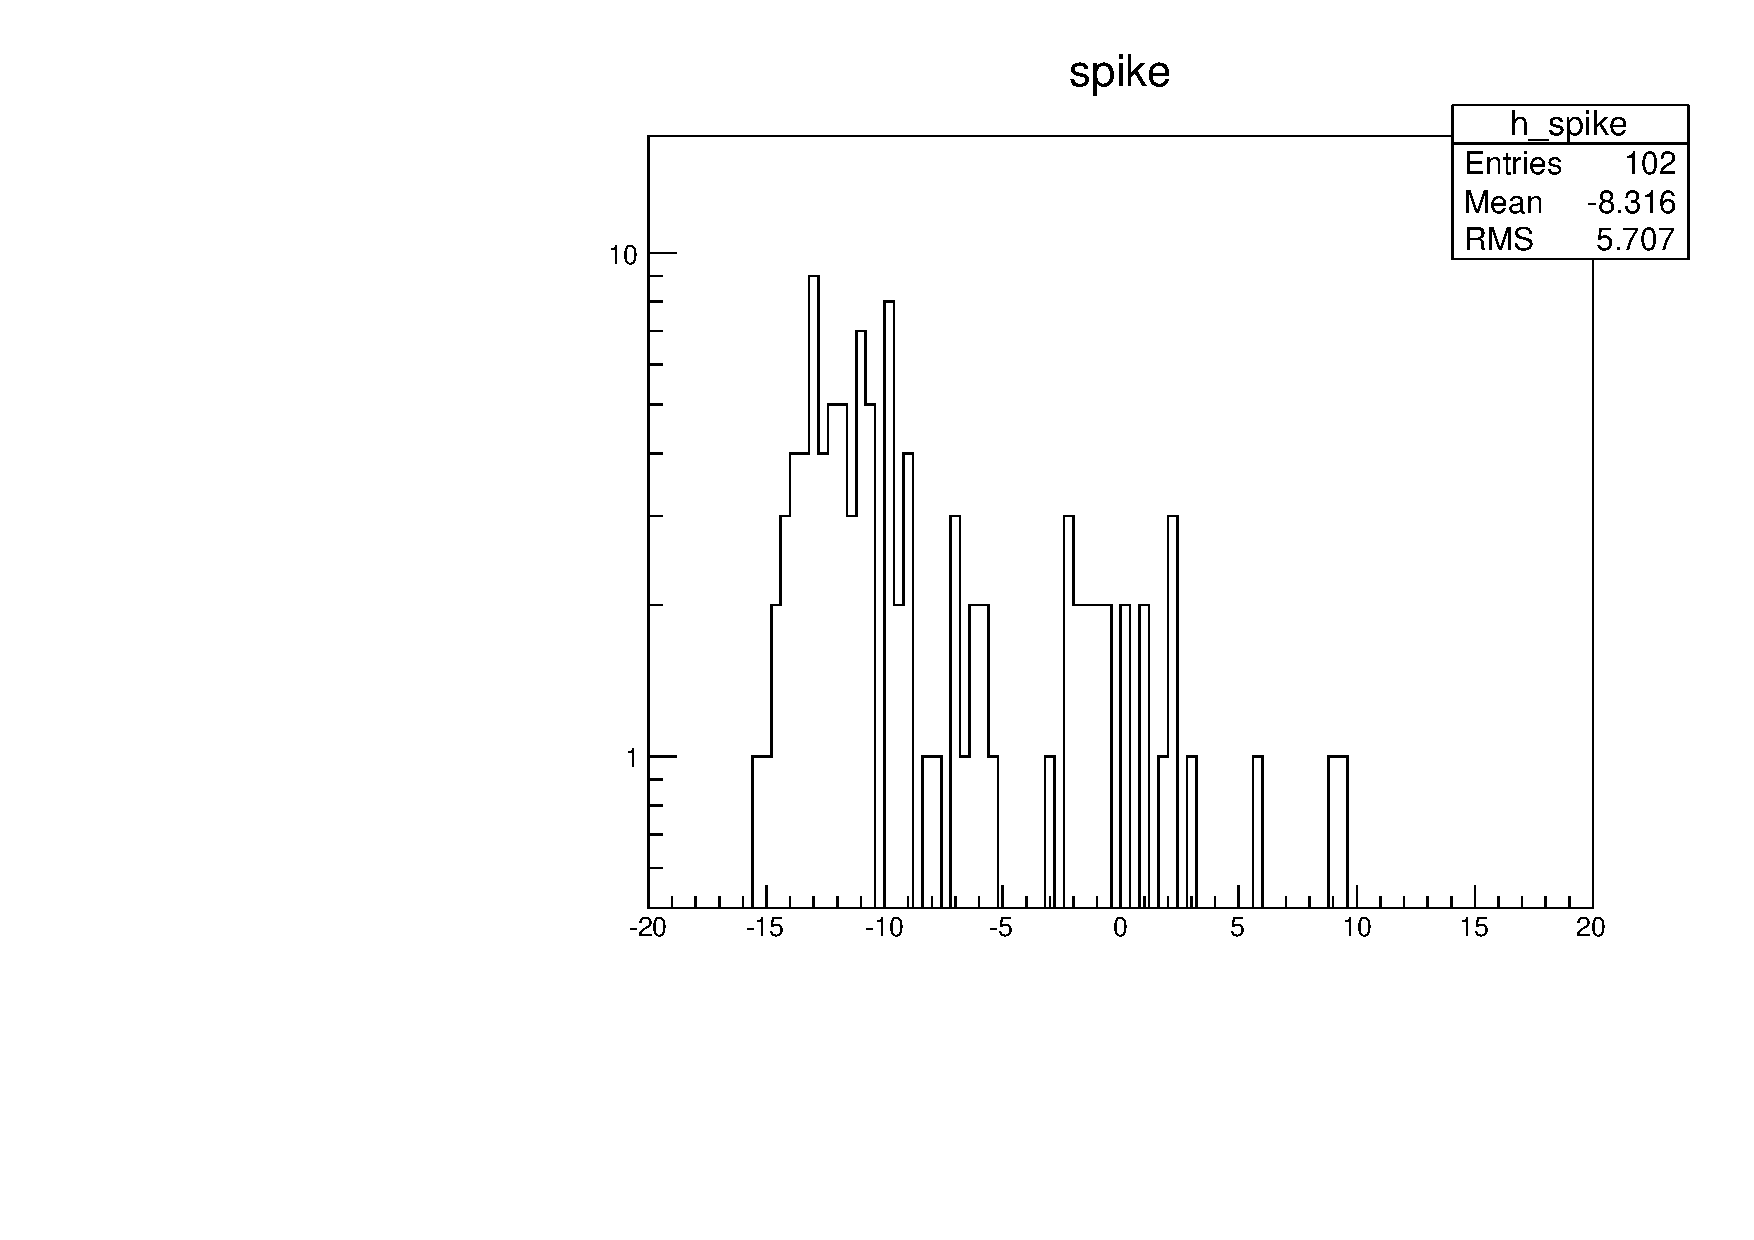
\includegraphics[width=0.45\textwidth]{analysis_figs/spike.pdf}}
{\label{fig:PromptTempl}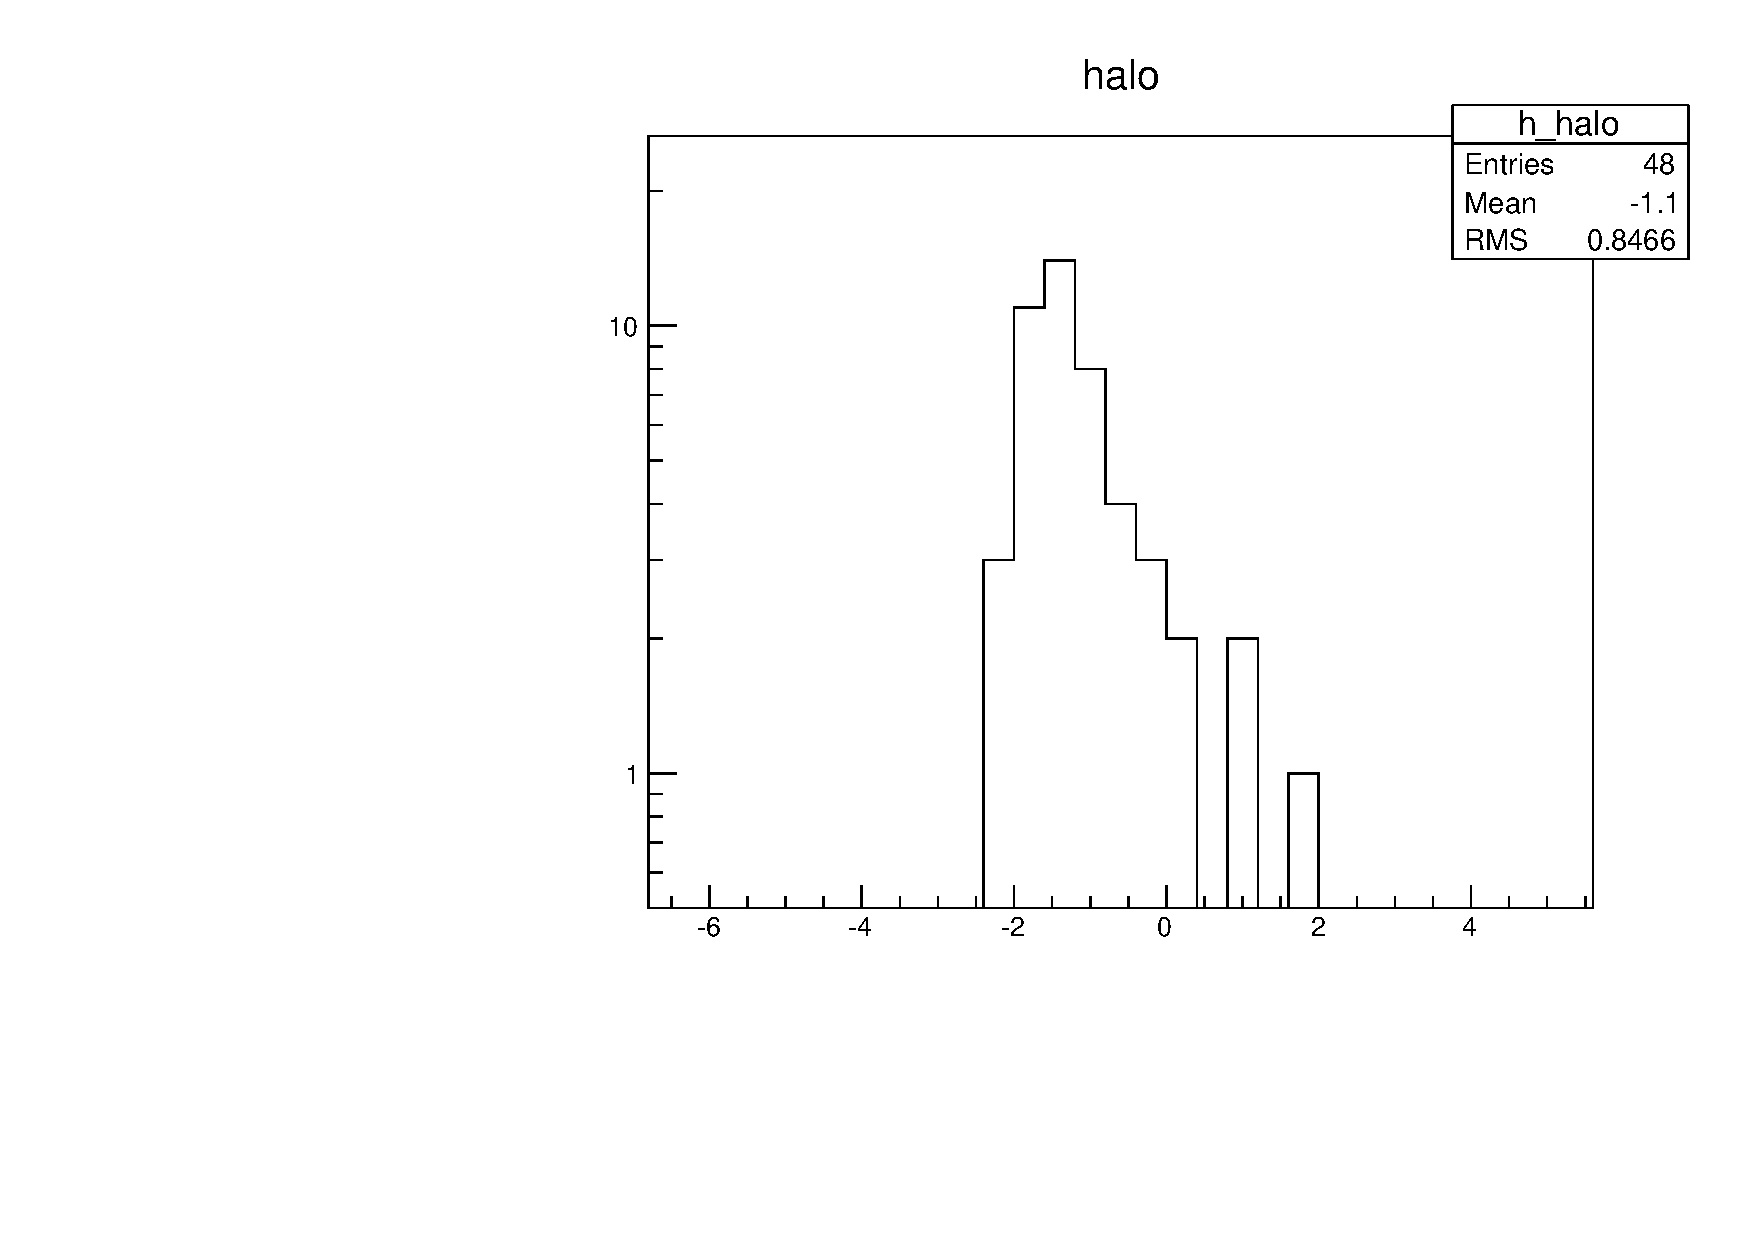
\includegraphics[width=0.45\textwidth]{analysis_figs/halo.pdf}}
\caption{Seed time distribution (ns) for spike and halo events}
\end{figure}

We estimate the final number of each non collision background events in data by the fitting the template distributions of spikes, beam halo and prompt to the complete timing distribution of the candidate events. Through this, we observe that the spike hypothesis is almost completely rejected, where the beam halo contribution is on the order of $< 1$ \% of the total expected events. Due to these results we have decided to neglect non-collision backgrounds in any further calculations.

\begin{figure}[h]
\centering
{\label{fig:can}\includegraphics[width=0.45\textwidth]{analysis_figs/cadidate.pdf}}
{\label{fig:fit}\includegraphics[width=0.45\textwidth]{analysis_figs/final_fit.pdf}}
\caption{Template fits to the candidate selectiona and model independent analysis selection.}
\label{fig:beamhalo}
\end{figure}


\subsection{Monte Carlo Backgrounds}
\label{sec:mcbackgrounds}

In our analyis for some of the SM backgrounds we rely on MC simulation. These backgrounds have gone through the full detector simulation where hadronization performed with PYTHIA parton shower. Such backgrounds have been corrected for various effects including pile up conditions and next-to-leading-order (NLO) effects. In this section we will discuss these effects in detail for some of the following backgrounds:

\begin{itemize}
\item $Z\rightarrow \nu\nu +\gamma$
\item $W\rightarrow l\nu + \gamma$
\item $Z(\rightarrow ll)+\gamma$
\item $\gamma$ + jets
\item $\gamma \gamma$
\item $W\rightarrow \mu (\tau) \nu$
\end{itemize}

%As the \zinvg and \winlvg processes are the main backgrounds of the analysis, a particular attention is required to correctly estimate their contribution to the observed number of events. \zinvg and \winlvg MC samples are 

\subsubsection{Z$\gamma$ and W$\gamma$}

One of the main backgrounds in this anlaysis is the irreducible background of Z$\gamma$. In order to account for all Z$\gamma$ channels we initially used an inclusive sample. However, upon further study we noticed the sample did not include Z$\to \tau\tau$ decays and was therefore not completely inclusive. To account for this we separate our backgrounds into Z($\to ll$)$\gamma$ and Z($\to \nu\nu$)$\gamma$ using generator-level information and added only selected the invisible part of the decay and added the leptonic part of the decay through another MC sample.

Both Z$\gamma$ and W$\gamma$ samples were simulated at the leading-order (LO) level using MadGraph and PYTHIA, including diagrams with up to two jets at the generator-level to be able to mimic the NLO contributions to the original process. 
%For these samples PYTHIA parton showering was used for the hadronization. 
Although these samples were designed to mimic NLO effects, we calculate more accurate NLO cross sections using the MCFM generator. In order to calculate the true NLO cross sections of the samples at hand, we have translated the Madgraph run cards used to produce the samples to MCFM cards. We have calculated NLO cross sections with MCFM in four different dynamical energy scaling: 

\begin{itemize}
 \item \texttt{sqrt(M$^2$+pt$_5^2$)}=$\sqrt{M_Z^2+p_{T,\gamma})^2}$,
 \item \texttt{m(345)}$=(p_\nu + p_{\bar \nu} + p_{\gamma})^2$,
 \item  \texttt{pt(photon)}$=p_{T,\gamma}$,
 \item \texttt{HT}$=p_{T,\nu} + p_{T,\bar \nu} + p_{T,\gamma}$.
 \end{itemize}


The difference in the cross section due to the choice of scale is used as systematic uncertainty.

Additionally, to correctly account for the systematics due to the PDF choice and the uncertainty on the measured value of the strong coupling $\alpha_s(m_Z)$, we followed the prescriptions of the PDF4LHC Working Group \cite{bib:PDF4LHC}. In particular, they recommend using an envelope technique to conservatively combine the $PDF+\alpha_S$ systematics coming from three PDF sets (CT10, MSTW2008 and NNPDF21)\footnote{We denote $X_0^{(i)}$ as the central values of $i =$ CT10, MSTW, NNPDF as calculated by MCFM, with $\sigma^{\pm (i)}_{PDF+\alpha_s}$ their uncertainty. A conservative prediction can be made by computing the maximum and minimum of the combined PDF$+\alpha_s$ uncertainties and defining a mid-point as being halfway in between these values:

\begin{align}
U = & \max_{i} \left\lbrace X_0^{(i)}+\sigma^{+ (i)}_{PDF+\alpha_s}\right\rbrace \\L = & \min_{i} \left\lbrace X_0^{(i)}-\sigma^{- (i)}_{PDF+\alpha_s}\right\rbrace \\
M = & \frac{U+L}{2}
\end{align}

with $U$, $L$ the upper and lower edges of the envelope and $M$ their mid-point.}.

We have so far only worked with the CT10 PDF set and the resulting cross sections in different dynamical scales along with the statistical and systematic uncertaintiy related to the PDF Analysis are shown in Table \ref{tab:znng} and \ref{tab:wg}. We have assigned the cross section using the m(345) scale as nominal cross section for the process, and assigned conservative 3\% systematics on the cross section  based on the average of the different dynamic scales. We further assigned 4\% systematics due to the pdf choice.

\begin{table}[h!]
\caption[]{Cross sections with systematic uncertainties for the \zinvg (left) processes using MCFM and CT10 PDF Library.}
\label{tab:znng}
\begin{center}
\begin{tabular}{ |c|c| } \hline
Dynamic scale  & PDF Analysis Central Value $\pm$ Stat $\pm$ Sys (fb) \\ \hline \hline
HT &  $ 31972.514  \pm  435.833 \pm  1229.045$ \\ \hline 
sqrt(M$^2$+pt$_5^2$) & $23683.579 \pm 405.517 \pm 1188.268$\\ \hline
m(345)  &  $34924.232 \pm 357.516 \pm 1285.799$\\ \hline
pt(photon)  & $ 38024.464 \pm 403.192 \pm 1576.783$\\ \hline \hline
% Full & $  $ \\ \hline
\end{tabular}
\end{center}
\end{table}

\begin{table}[h!]
\caption[]{Cross sections with systematic uncertainties for the  \winlvg processes using MCFM and CT10 PDF Library.}
\label{tab:wg}
\begin{center}
\begin{tabular}{|c|c|} \hline 
Dynamic scale  & PDF Analysis Central Value $\pm$ Stat $\pm$ Sys (fb) \\ \hline \hline
HT &  $ 561301.275 \pm  17510.088 \pm  19292.439$ \\ \hline
sqrt(M$^2$+pt$_5^2$) & $452394.411 \pm 14924.862 \pm 16069.347 $\\ \hline
m(345)  &  $ 599252.823 \pm 26582.388 \pm 22515.339$\\ \hline
pt(photon)  & $ 455729.856 \pm 15473.616 \pm 18160.944$\\ \hline \hline
%Full & $  $ \\ \hline
\end{tabular}
\end{center}
\end{table}


\subsection{Photon + Jet Background}

%On the other hand, the $\gamma$ + jet background is a significant contribution to our final state due to the large production cross section. We correct the normalization and the shape of the $\gamma$ + jet background through a reweighting method. The overall cross section normalization is discussed in the earlier section through a prescaled trigger control region. The shape normalization will be explained in Sec.~\ref{sec:control}.

Photon + Jet background has a large production cross section and is the leading background in the preselection level. We have tested various MC simulations generated with different generators to ensure good modeling of this background. We have observed the changing from Pythia to Madgraph generator reduces the discrepancy in the multiple jet bins (along with the overall yields, madgraph has ~30\% more events then pythia). This effect has been also observed by the \met POG as documented in the \met performance paper \cite{metperformance}. 

\begin{figure}[!h]
 \centering
  {\label{fig:madgraph}\includegraphics[width=0.45\textwidth]{analysis_figs/pythia.pdf}}
  {\label{fig:pythia}\includegraphics[width=0.45\textwidth]{analysis_figs/madgraph.pdf}} 
 \caption{Number of Jets above 30 \GeV for Pythia (left) and Madgraph (right) simulation samples}
 \label{fig:njets}
\end{figure}     

We have also observed that the discrepancy in 0 jet bin remained even with the $\gamma + \met$ madgraph sample. Therefore in conclusion we don't have a precise MC Simulation based way of estimating $\gamma + \met$ background rate. Therefore we have decided to construct a control sample where we measure the rate of this background with respect to data in different jet bins using the jet binning definitions given in Section 4.5 .

In this control sample, we have selected events triggered only by the prescaled single photon trigger. By going to a prescaled trigger, we would only have $20\%$ of the full data however, this way, we won't have any restriction on the $\met$ coming from to the trigger. To get to a region completely orthogonal to our signal selection,  we required $\met < 40.$. In this region we look at the $\gamma + jet$ production, in 2 different jet bins, by normalizing the expected yields to data after subtracting all other backgrounds from the data. The overall distributions can be seen in Fig.~\ref{fig:control_prescale1}. Based on these distributions, we have scale up the $\gamma + jet$ cross section in 0 Jet bin catagory by 1.7 and greater than 0 Jet bin catagory by 1.1. 


\begin{figure}[!h]
 \centering
  {\label{fig:madgraph}\includegraphics[width=0.45\textwidth]{analysis_figs/prescale_pt.pdf}}
  {\label{fig:pythia}\includegraphics[width=0.45\textwidth]{analysis_figs/prescale_njet.pdf}}
 \caption{Photon Pt (left) and NJets (right) distribution for the control region. }
 \label{fig:control_prescale1}
\end{figure}

\subsection{Other MC Backgrounds}

The other MC backgrounds that we use are W$\to \mu\nu$ and W$\to \tau\nu$ and $\gamma$ + Jets. We do not apply any factors for the Wl$\nu$ backgrounds, as are significantly reduced with lepton vetos. However due to avoid overlaps with the data driven jet fake background, we have only considered the leptonic decays of W$\to \tau\nu$ background, explicitly removing the hadronic part. 


